\documentclass[a4paper, twoside]{NUSThesis}
\usepackage[
backend=biber,
style=nature,
%citestyle=numeric,
giveninits=true,
doi=false]{biblatex}
%\DeclareFieldFormat*{title}{``#1''\newunitpunct} % move comma outside the quotation mark
\addbibresource{references.bib}
\usepackage[PetersLenny]{fncychap}
%\ChNumVar{\fontsize{60}{70}\rm\textcolor[rgb]{.21, .34, .50}}
\renewcommand{\TL}[1]{\color[HTML]{888888}\setlength{\tl}{#1}}
\ChNameVar{\color[HTML]{888888}\fontsize{14}{16}\rm}
\ChNumVar{\fontsize{60}{62}\rm\color[HTML]{888888}}
\ChTitleVar{\huge\notosans\bfseries\color[HTML]{000000}}
%\ChTitleVar{\huge\bfseries\sf}
\usepackage{pkg_def}
\usepackage{thesis_sym}

\usepackage{calligra} % for dedication

\title{Modeling Nonlinear Optical Response in 2D materials from Nonequilibrium Quantum Dynamics}
\author{Wenwen Mao}
\prevdegrees{Universität Hamburg}
\degree{Erlangung des Doktorgrades}
\field{der Fakultät für Mathematik, Informatik und Naturwissenschaften, Fachbereich Physik}
\degreeyear{2023}

\supervisor{Professor Angel Rubio\\Assitant Professor Shunsuke Sato}

% only involve the examiners in the final submission
\examiners{%
    Professor YAN Jie\\
    Associate Professor Andrivo RUSYDI\\
    Assistant Professor WONG Liang Jie, Nanyang Technological University}

\hypersetup{
    pdfauthor={Wenwen Mao},
    pdftitle={Modeling Nonlinear Optical Response in 2D materials from Nonequilibrium Quantum Dynamics},
}

%\hyphenation{thatshouldnot}
%\usepackage[none]{hyphenat}
\begin{document}
\maketitle
\makedeclaration
\frontmatter

\begin{acknowledgments}
    First, I would like to thank my supervisors Angel Rubio and Shunsuke Sato for their continuous support of my Ph.D
\end{acknowledgments}
\clearpage
\begin{dedication}
    \calligra \large To my
\end{dedication}
\clearpage
{
    \hypersetup{linkcolor=[rgb]{.21, .34, .50}}
    \tableofcontents
\cleardoublepage
\begin{abstract}
Through the exploration of high-order harmonic generation, this research contributes to the broader scientific community's knowledge and paves the way for new discoveries and technological breakthroughs. The study of HHG not only deepens our comprehension of fundamental physics but also holds great promise for revolutionizing various fields, ranging from materials science and chemistry to biology and quantum technologies.
\end{abstract}
\listoftables
\listoffigures
}
\printglossary[type=symbols, style=long, title={List of Abbreviations}]
\mainmatter
%\chapter{Background and Theory}
\label{ch:background}
The theoretical concepts of this thesis are overviewed in this chapter.
In an XFEL SPI experiment, single particles are illuminated by high-intensity coherent X-ray pulses
(\cref{fig:SPI_experiment}). 
We will describe how, on the basis of X-ray scattering theory, the structural information of molecules in SPI experiments is encoded\cite{lohReconstructionAlgorithmSingleparticle2009} in a sparse diffraction pattern--- Poisson sampled Ewald sphere slices of the
diffraction intensity with unknown orientations.

The XFEL SPI is an inverse problem of this encoding procedure and typically consists of
two steps in the data analysis pipeline: 
\begin{enumerate}
    \item diffraction intensity reconstruction: rebuild the three dimensional
        intensity distribution from sparse two dimensional diffraction patterns by assuming
        the diffraction intensity is continuous;
    \item phase retrieval: as the diffraction intensity only records the magnitudes information of
        the Fourier transform of the scattering factor with phase information missing recover
        the missing phase in the diffraction intensity by using prior information of the sample, such
        as size.
\end{enumerate}
In this thesis, we mainly focus on the data analysis and will provide needed theoretical and algorithmic
tools in the rest of this chapter.


\section{Basics of X-ray scalar diffraction theory}
\label{sec:scattering_diffraction}

In this section, we briefly describe the basics of X-ray diffraction to 
model the relation between structural information of single particles and 
their diffraction patterns recorded in experiment.

The interaction cross-section between photons and electrons essentially
consists of three parts when the energy of photons is in the range from
\SI{200}{eV} to \SI{500}{keV} \cite{raubenheimerLCLSIIStatusCW2015}:
\begin{enumerate}
    \item \emph{photoelectric effect}: core electrons are ejected by absorbing the
        energy of photons which cause vacancies. The photons are emitted 
        randomly when vacancies are filled another electrons;
    \item \emph{coherent scattering}: in this process, the total energy is conserved when photons
        are scattered by electrons. Those photons are coherent and their phases are decided by
        their relative position where they are scattered;
    \item \emph{Compton scattering}: this is an incoherent scattering process in which the incident photon transfers some of its energy to the electron.
\end{enumerate}

Taking the LCLS-II as an example\cite{raubenheimerLCLSIIStatusCW2015},
the photon energy range of SPI experiment with XFEL is around \SI{200}{eV} and
\SI{25}{keV}. In this range, the recorded photons are mainly from coherent
scattering\cite{hubbellReviewPhotonInteraction1999}. The fluorescence photons
(photoelectric effect) add an incoherent background to the diffraction patterns
and Compton photons are negligible. 

A classical model is adopted to illustrate the coherent scattered photons
encode particles' structures into their scattered angles and amplitudes.
When an electron (at the origin) is experiencing an oscillating incident plane electromagnetic wave, $\bvec E_\text{in}$,
it also emits electromagnetic radiation whose electric field part at the position $\bvec x$ could be expressed as
\begin{equation}
    \bvec{E}_\text{e}(\bvec x)=\frac{e^2}{4 \pi \varepsilon_{0} m_\text{e} c^{2}}
    \frac{\bvec{x} \times(\bvec{x} \times
    \bvec{E}_{\text{in}})}{|\bvec{x}|^{3}}\text{,}
    \label{eq:Esc}
\end{equation}
where $\varepsilon_{0}$ is the vacuum permittivity, $e$ and $m_\text{e}$ represent the charge and mass of electron respectively.
More often, the classical electron radius\cite{griffithsIntroductionQuantumMechanics2014}
\begin{equation}
    r_\text{e}=\frac{e^{2}}{4 \pi \varepsilon_{0} m_\text{e} c^{2}} \approx \SI{2.818e-15}{m}
    \label{eq:re}
\end{equation}
is introduced to simplify \cref{eq:Esc}. 
Multiple scattering of incident beam is ignored here since the specimen used in XFEP SPI experiment
is optical thin\cite{thibaultAlgorithmicMethodsDiffraction2007}.

In the XFEL SPI experiment (\cref{fig:lab_frame}), the distance between the illuminated particle and an observation point
on the detector, $R \sim \SI{1}{m}$, is several orders of magnitudes larger than
the scale of a nano-sized particle ($\sim\SI{10}{nm}$). Therefore, under the far field approximation\cite{jacksonClassicalElectrodynamics2007},
the electric field scattered by a particle with electron 
density $\rho(\bvec x_\text{p})$ at $\bvec x_\text{d}$ (usually the position of a detector pixel) 
is given by
\begin{equation}
    \bvec{E}(\bvec x_\text{d})=r_\text{e} \frac{\bvec x_\text{d} \times\left(\bvec x_\text{d}
    \times \bvec{E}_{\text{in}}\right)}{|\bvec x_\text{d}|^{3}}
    \int \rho(\bvec x_\text{p}) \exp\bigl[-2 \pi \img(\bvec k_\text{out} - \bvec k_\text{in})
    \cdot \bvec x_\text{p}\bigr] \dif \bvec x_\text{p} 
    \label{eq:Esc_int}
\end{equation}
where $\bvec k_\text{out}$ and $\bvec k_\text{in}$ are the scattered and incident wave vector, and
$(\bvec k_\text{out} - \bvec k_\text{in}) \cdot \bvec x_\text{p}$ is the difference between two
optical paths passing the origin and $\bvec x_\text{p}$.
Owing to the conservation of energy in elastic scattering, the wavelength of the scattered photon
is the same as the incident photon, or $\envert{\bvec k_\text{out}} = \envert{\bvec k_\text{in}}=
1/\lambda$, where $\lambda$ is the wavelength of X-ray, and the direction of $\bvec k_\text{out}$
is the same as the direction $\bvec x_\text{d}$. By introducing a new vector,
\begin{equation}
    \bvec k = \gls{torec}(\bvec x_\text{d}) = \bvec k_\text{out} - \bvec k_\text{in} = \envert{\bvec k_\text{in}}\hat{\bvec x}_\text{d} - \bvec k_\text{in}
    \label{eq:def_Krec}
\end{equation}
where $\hat{\bvec{a}}$ indicates the direction unit vector of a vector $\bvec{a}$,
and the Fourier transform of $\rho(\bvec x)$,
\begin{equation}
    \tilde{\rho}(\bvec k) = \Fourier[\rho](\bvec k)= \int \rho(\bvec x_\text{p}) \exp(- 2 \pi
    \img\bvec{k} \cdot \bvec x_\text{p}) \dif \bvec x_\text{p}\text{,}
    \label{eq:FT_rho}
\end{equation}
\cref{eq:Esc_int} could be rewritten as
\begin{equation}
    \bvec E(\bvec x_\text{d}) = \bvec E_\text{e} (\bvec x_\text{d})\cdot \tilde{\rho}\circ
    \torec(\bvec x_\text{d})\text{,}
    \label{eq:Esc_int2}
\end{equation}
where $E_\text{e}$ is defined in \cref{eq:Esc}.

%\Cref{eq:Esc_int} actual holds an assumption that electron density $\rho$ is independent on time.
%In other words, particle is frozen when it is illuminated by an XFEL pulse. 

%First, the thermal
%motion of particles could be neglected. For example, the weight $m$ and radius of gyration
%$r_\text{g}$ of lysozyme are \SI{14400}{\kilogram \per \kilo\mole} and
%\SI{15.20}{\angstrom}\cite{heNovelCorrelationProtein2003}.  In room temperature, the magnitude of
%thermal motion in \SI{1}{\femto\second}, including translation and rotation, is about
%\SI{1e-4}{\angstrom} by considering $3 k T / 2 = m v ^2/2 = m r_\text{g}^2 \omega^2 /2$, where $k$,
%$T$ are the Boltzmann constant and temperature, $v$ and $\omega$ are linear and angular speed. The
%angular speed is converted to linear speed by multiplying the radius of gyration. The value
%\SI{1e-4}{\angstrom} are much smaller than the radius of hydrogen atom (about
%\SI{1e-1}{\angstrom}). Second, the radiation damage on sample was studied with computer simulation
%in \cite{neutzePotentialBiomolecularImaging2000}.  Many facts are included: photoelectric, elastic
%and Compton scattering.  This study indicates that the damage could be outrun if pulse length is
%short enough.

The new vector, $\bvec k$, in \cref{eq:def_Krec} is a sphere centered at $\bvec k_\text{in}$ with
radius $1/\lambda$, which is known as \emph{Ewald sphere}.  The space of wave vectors is called
\emph{reciprocal space} (\cref{fig:lab_frame}), $\bbR_\text{rec}^3$ and the map between the laboratory frame
$\bbR_\text{lab}^3$ to the Ewald sphere in reciprocal space is denoted as $\torec$.

\begin{figure}[htpb]
    \centering
    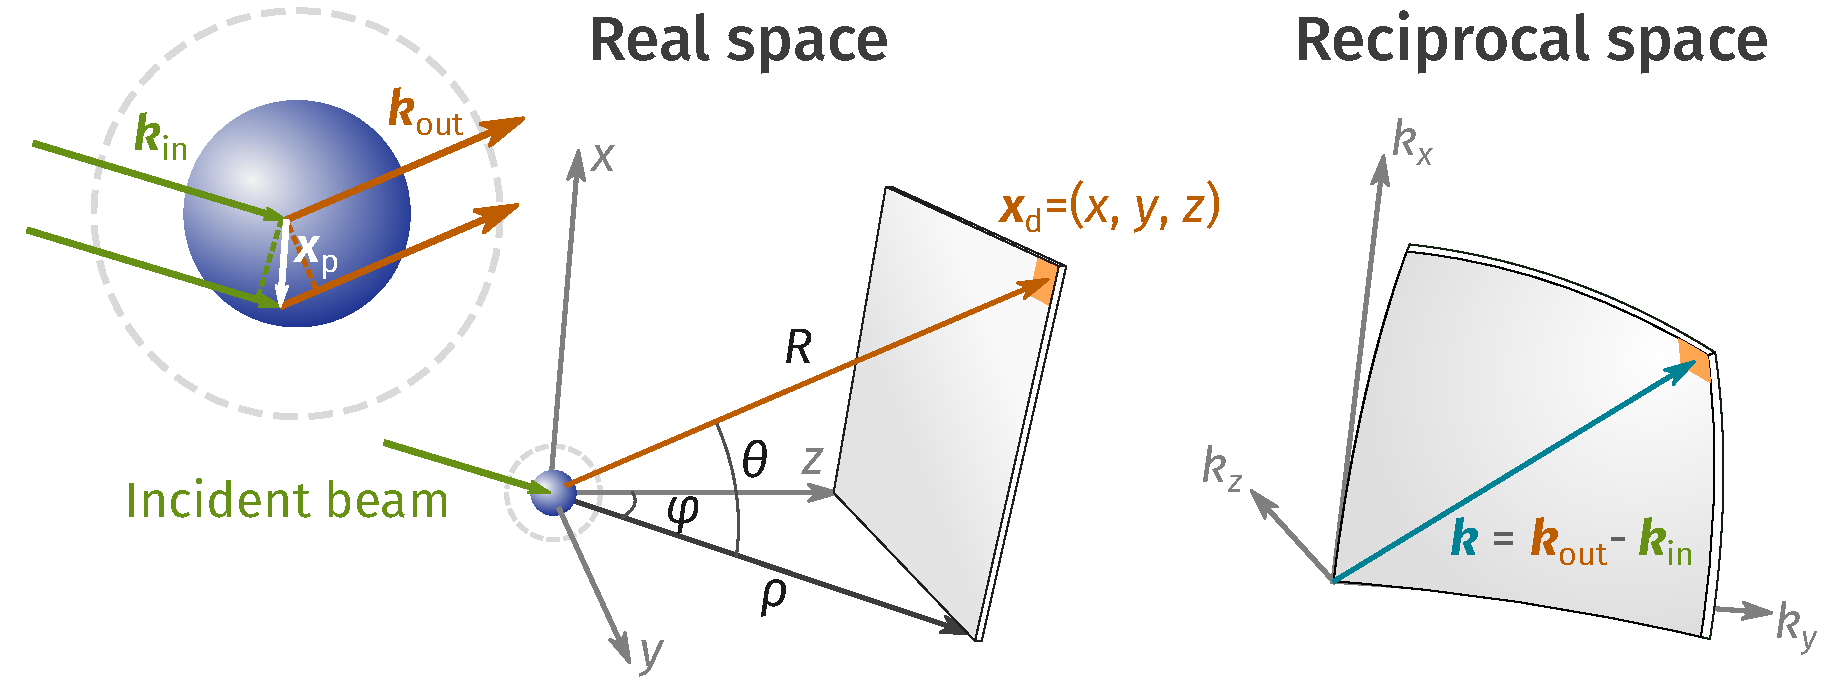
\includegraphics[width=0.96\textwidth]{pic/ill_lab.pdf}
    \caption[Lab coordinate system]{This figure illustrates the coordinate system of the real
        space (laboratory frame) and the reciprocal space and also shows the transformation between them.}
    \label{fig:lab_frame}
\end{figure}

%%----------------------------------------------------------------------------------------
% CHAPTER ONE
%----------------------------------------------------------------------------------------


\chapter{INTRODUCTION }
\label{ch:introduction}
In the conventional understanding of linear optics, the response of a material to an incident
electromagnetic wave is linearly proportional to the strength of the electric field. However, when
the intensity of the incident light becomes strong enough, the nonlinear optical response
becomes significant. This regime reveals a rich variety of phenomena, including the photoncarrier
injection, phase modulation, and harmonic generation.
After the first observation of nonlinear optical phenomena by Franken~\cite{franken1961generation},
based on recent advancements in laser technology, groundbreaking research in the field of nonlinear
optics have been driven~\cite{RevModPhys.72.545, RevModPhys.81.163, MOUROU2012720}, have conducted in a new era of intense light generation. These developments have paved the way for in-depth exploration of light-matter interactions in highly nonlinear regimes both in atomic and condensed matter phases. One of the most captivating nonlinear optical phenomena made accessible by these advances is High-order Harmonic Generation (\gls{HHG}), a process characterized by its extreme photon upconversion and remarkable nonlinear characteristics.

This thesis aims to provide a comprehensive overview of the nonlinear response phenomenons
including photocarrier injection and high-order harmonic generation from a theoretical point of view linked to the microscopic modeling of the electron dynamics in those 2d quantum materials. We will explore the theoretical foundations of light induced time-dependent quantum
dynamics evolution in solid systems,
including the quantum mechanical description of the light-matter ineraction process and the role of
excited electron dynamics.  By investigating photocarrier injection and HHG, we seek to deepen our understanding of the nonlinear optical response of materials and unlock the potential for applications in fields such as ultrafast spectroscopy, attosecond science, and advanced imaging techniques.
%=====================================================================================================================================
\section{Nonlinear Optical Response}
In studies of optical response theory within solid systems, the dielectric function serves as an centered concept, the dielectric function characterizes how the material's polarization, induced by the external field, evolves with the field's frequency and intensity. Mathematically, the dielectric function connects the material's polarization density to the electric field through Maxwell's equations, forming the basis for understanding its optical properties. Linear response theory, predicated on the assumption of weak perturbations, asserts that the induced polarization is directly proportional to the strength of the applied field.
Linear response theory is most applicable when the perturbations are weak. In other words, the system's behavior is approximately linear in the vicinity of its equilibrium or initial state.
In such cases. the system's behavior is described by linear susceptibility ($\chi^{(1)}$).

The electric susceptibility ($\chi^{(1)}$) describes the response of a material to an applied electric field ($\mathbf{E}$). The relationship between the induced polarization ($\mathbf{P}$) and the applied electric field can be expressed as:

\begin{equation}
	\mathbf{P^{(1)}(t)} =\epsilon_0 \int_{0}^{\infty}\mathbf R^{(1)} \cdot \mathbf{E}(t-\tau)d\tau
	\label{eqn:linearresponse}
\end{equation}
Where:
\begin{itemize}
	\item $\mathbf{P}$ is the induced polarization vector,
	\item $\mathbf R^{(1)}$ is the linear response function, electric susceptibility tensor, and
	\item $\mathbf{E}$ is the applied electric field vector.

\end{itemize}
Equation.~(\ref{eqn:linearresponse}) can be transformed to the frequency domain by intoducing the
Fourier trasnform of electric field:
\[
	E(\omega) =\int_{-\infty'}^{\infty}E(t) \cdot e^{i\omega t} dt.
\]
\[
	E(t) =\frac{1}{2\pi}\int_{-\infty'}^{\infty}E(\omega) \cdot e^{-i\omega t} d\omega.
\]
By introducing above Fourier transform, we have:
\[
	\mathbf P^{(1)}(t) =\epsilon_0 \int_{-\infty}^{\infty} \frac{d\omega}{2\pi} \int_{0}^{\infty}\mathbf R^{(1)} e^{i\omega \tau} \cdot \mathbf{E}(\omega) e^{-i\omega t} d\tau
\]
we intoduce an explicit expression for the linear susceptibility is:
\[
	\chi^{(1)}(\omega;\omega) =\int_{0}^{\infty}\mathbf R^{(1)}(\tau) \cdot e^{i\omega \tau} d\tau.
\]
By noting that the equality must be maintained for each frequency $\omega$, we recover the usual
frequency domain description of linear response:

\begin{equation}
	\mathbf{P}^{(1)}(\omega) =\epsilon_0 \chi^{(1)}(\omega;\omega) \cdot \mathbf{E}(\omega)
	\label{eqn:linearresponse-W}
\end{equation}
In nonlinear response, the relationship can be described by analogous procedures. We can express the nonlinear polarization $P_i(t)$ as a convolution integral involving the electric field $E_j(t)$ and the time-dependent response function $\chi^{(2)}_{ijk}(t-t_1,t-t_2)$ for the second-order nonlinear process:
\[
	P_i(t) = \epsilon_0 \sum_{j=1}^{3} \sum_{k=1}^{3}\int_{-\infty}^t \int_{-\infty}^t \, \chi^{(2)}_{ijk}(t-t_1,t-t_2) E_j(t_1)E_k(t_2) dt_1 dt_2
\]
We should make clear that the first order liner effect as one connects materials properties linearly changing with applied field and should not apply in general for describing strong non linear phenomena im materials where one has to go beyond the description to nonlinear response theory. When considering the time-domain response of a material to an external perturbation, one deals frequency-dependent susceptibilities. These susceptibilities can be expressed in terms of tensor notation and integrated over frequency to account for the material's response over a range of frequencies. In the frequency domain, the induced polarization ($P$) can be expressed in terms of the applied electric field ($E$) and the susceptibility tensor as:

\[
	P_i(\omega) = \epsilon_0 \sum_{j=1}^{3} \sum_{k=1}^{3}\int\int \chi^{(2)}_{ijk}(\omega, \omega_1, \omega_2) E_j(\omega_1) E_k(\omega_2) \, d\omega_1 \, d\omega_2
\]

Where:
\begin{itemize}
	\item $P_i(\omega)$ is the induced polarization component at frequency $\omega$ along direction
	      $i$,
	\item $\chi^{(2)}_{ijk}(\omega, \omega_1, \omega_2)$ is the frequency-dependent second-order susceptibility tensor,
	\item $E_j(\omega_1)$ and $E_k(\omega_2)$ are the components of the applied electric field at frequencies $\omega_1$ and $\omega_2$ respectively, and
	\item The integral is taken over all possible frequencies.
\end{itemize}

In summary, the nonlinear response of a material to external perturbations can be described using
tensor notation, incorporating frequency or time integrals to capture the material's response over
a range of frequencies or times. The high-order susceptibility tensor ($\chi^{(n)}$) plays a crucial role in characterizing this nonlinear response.
Frequency and Intensity-dependent absorption is a key feature of nonlinear response and is often exploited in applications such as laser-induced material processing.

%=========================================================================================================================================================
\section{Photocarrier Injection \label{sec:intro_photocarrier}}
\begin{figure}[htpb]
	\centering
	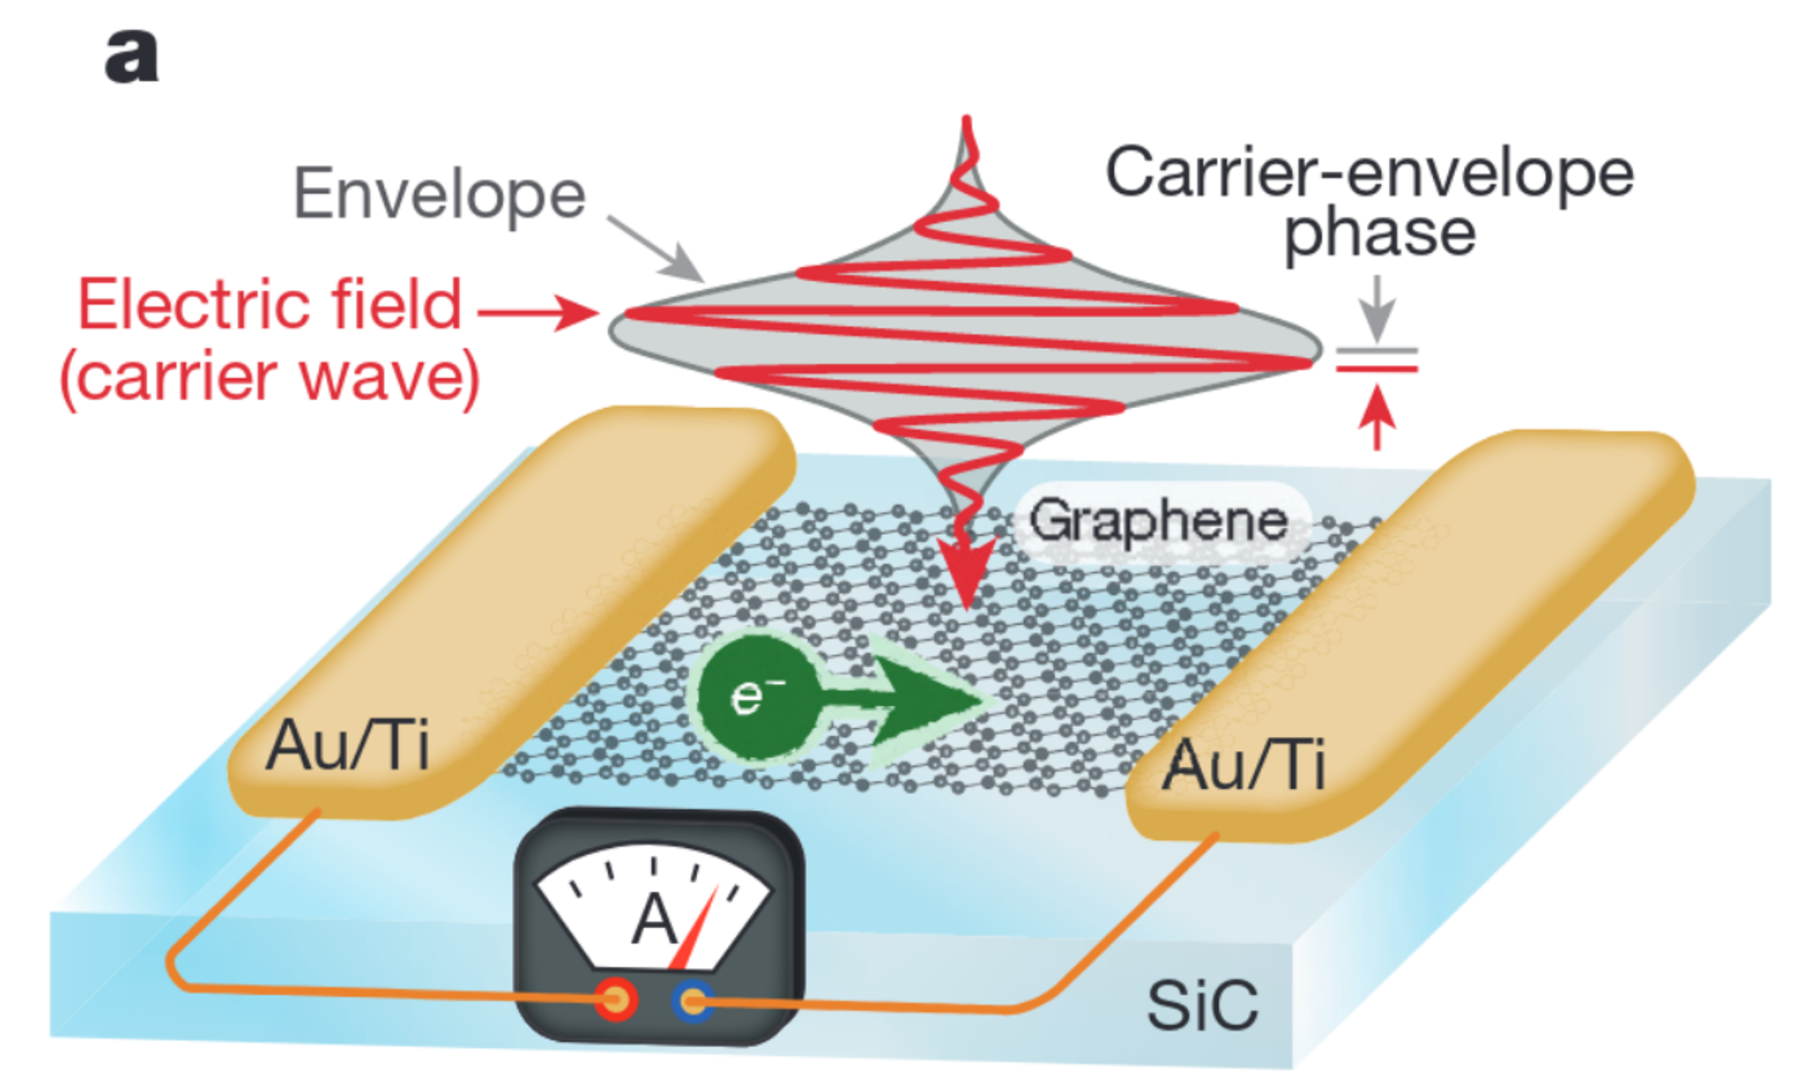
\includegraphics[width=0.8\textwidth]{pic/photocarrier_intro.pdf}
	\caption[Lab coordinate system]{Schematic of the experimental set-up in Light-field-driven currents in graphene ~\cite{Higuchi2017}, Copyright 2017, Nature, with a graphene strip on a SiC substrate under illumination of two-cycle laser pulses with controlled CEP. The CEP-dependent current is measured.}
	\label{fig: photocarrier_intro}
\end{figure}
\textcolor{red}{Photocarrier injection is a phenomenon in semiconductor physics and optoelectronics where photoexcited carriers (electrons and holes) are injected into a semiconductor material due to the absorption of photons.  When light is incident on a semiconductor material, it generates electron-hole pairs, creating an excess of carriers within the material. If the semiconductor is part of an electronic circuit, these excess carriers can contribute to the flow of electrical current. Figure.~\ref{fig: photocarrier_intro} illustrates the concept of photocarrier injection in a graphene strip under the illumination of two-cycle laser pulses with controlled carrier-envelope phase (CEP) in recent experimental set-up~\cite{Higuchi2017}. The injected currents have complex components, including a shif current  and injection current. The injection current persists even after the laser pulse has ended and it arises from the breaking of time-reversal symmetry through elliptically or circularly polarized light, as well as the breaking of intrinsic spatial inversion symmetry. The injection current is a manifestation of quantum interference between various excitation pathways, leading to a polar distribution of electrons or holes in momentum space. Shift current, also known as displacement current, refers to a nonlinear optical response observed in materials with broken inversion symmetry when subjected to an oscillating electric field. Shift current arises due to the displacement of charge within the material in response to the changing electric field, rather than the flow of charge carriers as in conventional currents.}

For the photovoltaic injection in bulk systems, the second-order nonlinear optical effect, as explored in~\cite{PhysRevB.61.5337}, has garnered considerable attention for its potential in achieving highly efficient light-to-current conversion. Investigations into shift-current, detailed in references~\cite{PhysRevLett.107.126805,doi:10.1126/science.1168636,Yang2010,10.1063/5.0101513}, exemplify the significance of this phenomenon.

Another noteworthy aspect of second-order nonlinear current is the "injection
current"\cite{sipe2000second,laman2005ultrafast,
	10.1063/1.125084,PhysRevB.61.5337,10.1063/1.2131191}. This current can be induced by the
breaking of time-reversal symmetry through elliptically or circularly polarized light, in addition to the
breaking of intrinsic spatial inversion symmetry. The injection current results from the population
imbalance induced by quantum interference (\gls{QuI}) between various excitation paths, arising
from the interference between absorption pathways associated with orthogonal components of
polarization. Consequently, this leads to a polar distribution of electrons or holes in momentum
space, generating a current injection that temporally aligns with optical intensity. Remarkably,
the non-oscillating current induced by quantum interference may persist even after the perturbing
laser irradiation stops.

It is noteworthy that, unlike the shift-current occurs solely during laser irradiation, the injection current exhibits persistence even after the conclusion of laser irradiation. This enduring quality underscores the unique and sustained contribution of the injection current in the context of nonlinear optical effects.

Going, beyond second-order nonlinear effects, researchers have investigated into the realm of
photovoltaic effects induced by intense few-cycle laser
pulses~\cite{Schiffrin2013,PhysRevLett.113.087401,PhysRevLett.116.057401,Higuchi2017,Heide_2020,Morimoto_2022}.
Notably, such laser pulses possess the capability to extrinsically break spatial inversion
symmetry. In addition to this, the presence of a strong field introduces highly nonlinear
excitation channels, including pathways such as tunneling excitation. The combination of extrinsic spatial inversion symmetry breaking and intense nonlinear interactions between light and matter opens the possibility for an intense few-cycle laser pulse to induce a direct current (dc-current) even in a material with intrinsic inversion symmetry.


The uniqueness of the photovoltaic effect with a few-cycle pulse lies in its dependence on breaking the inversion symmetry of the incident light fields. This intrinsic connection allows for the manipulation of the induced current by controlling both the intensity and carrier-envelope phase of the pulse~\cite{Schiffrin2013,Higuchi2017}. The exploration of these intense few-cycle laser pulses not only expands the understanding of nonlinear optical phenomena but also unveils avenues for precise control and manipulation of induced currents through tailored light-matter interactions.


In recent research, an effective method for manipulating valley population has surfaced, centered
around the interplay of two circularly polarized lights with different frequencies, denoted as
$\omega$ and $2\omega$. This investigation is particularly fitting in the context of
two-dimensional systems~\cite{Jimenez-Galan2020,Mrudul:21}. Individually, each circularly polarized
light breaks time-reversal symmetry, and when combined, the fields exhibit the added capability of
breaking spatial inversion symmetry. This coupled contravention upon time-reversal and spatial
inversion symmetries gives rise to a population imbalance in momentum space upon laser excitation.
This, in turn, apperas as a sustained charge flow persisting even after the laser irradiation. Notably, this methodology has extended beyond theoretical exploration, with numerical studies incorporating first-principles calculations applied to bulk solids~\cite{PhysRevLett.127.126601}. The multifaceted approach of combining circularly polarized lights at different frequencies not only enriches our understanding of valley population dynamics but also holds promise for diverse technological applications in the realm of materials and quantum control phenomena.
%=========================================================================================================================================================
\section{High-order Harmonic Generation \label{sec: intro_hhg}}
\begin{figure}[htpb]
	\centering
	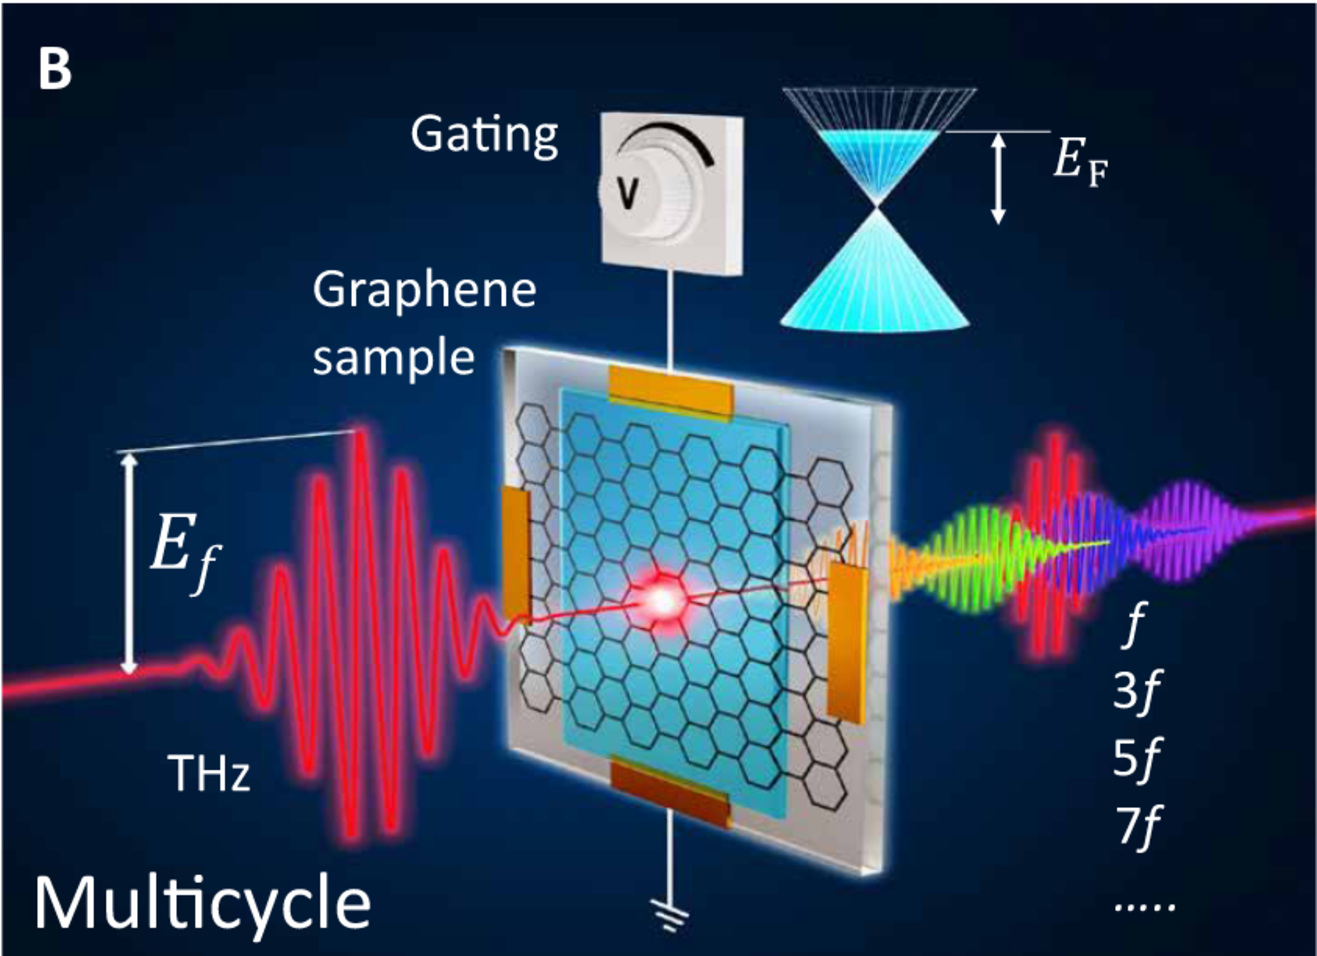
\includegraphics[width=0.8\textwidth]{pic/HHG_intro.pdf}
	\caption[Lab coordinate system]{Schematic of the experimental set-up in Schematic and main results of the THz high-harmonic generation in graphene sample. Electrical tunability of terahertz nonlinearity in graphene ~\cite{kovalev2021electrical}, Copyright 2021, Science Advances. Quasi-monochromatic, linearly polarized THz pump wave from the TELBE source is incident on a graphene sample, single-layer CVD-grown graphene deposited on SiO2 substrate. The incident THz field drives the nonlinear current in graphene, leading to re-emission at higher odd-order harmonics that appear in the spectrum of the transmitted THz signal.}
	\label{fig: HHG_intro}
\end{figure}
Traditional hgh-order harmonic generation (\gls{HHG}) is a phenomenon where intense laser light interacts with a gas, causing the generation of very high-frequency light waves. This process typically occurs when a strong laser field ionizes a material, causing electrons to be ripped away from atoms.
These electrons then undergo complex dynamics, involving acceleration, coherent motion, and recombination with their parent ions. Through this intricate dance, the electrons emit high-energy photons with frequencies much higher than that of the incident laser, often extending into the extreme ultraviolet (XUV) and X-ray regions of the electromagnetic spectrum \cite{gaumnitz2017streaking}.\\
\\
Since first observed in 1987 using rare gases as target specimens \cite{McPherson:87, Ferray_1988},  gas-phase HHG has been intensively utilized to generate ultrashort attosecond light pulses~\cite{PhysRevLett.68.3535, PhysRevLett.70.1599, PhysRevA.49.2117} for investigating ultrafast dynamics in matter in the time domain which is a typical time scale for the motion of electrons.\cite{baltuvska2003attosecond, Goulielmakis2010, doi:10.1126/science.1260311, doi:10.1126/science.aag1268}. HHG provides a unique window into electron dynamics and allows us to investigate processes occurring on attosecond timescales. The emitted harmonics carry valuable information about the electronic structure, band gaps, and transient states of the material, offering a powerful tool for probing and controlling ultrafast processes.
In recent years, there have been significant advancements in experimental techniques for studying high-order harmonic generation. The use of intense femtosecond laser pulses, pulse shaping methods, and advanced detection schemes have enabled precise control and characterization of the generated harmonics. These experimental advances have led to breakthroughs in attosecond science, providing tools for investigating ultrafast phenomena in a wide range of atoms ~\cite{Goulielmakis2010,PhysRevLett.105.143002,PhysRevLett.106.123601}, molecules~\cite{Warrick2016,Reduzzi2016,PhysRevResearch.3.043222}, and solids~\cite{doi:10.1126/science.1260311, doi:10.1126/science.aag1268, Mashiko2016,Siegrist2019, vampa2017merge}.
The HHG in solid-state systems was first observed in ZnO in 2011 in mid-infrared (MIR) laser field~\cite{Ghimire2011}, and it has since garnered significant attention, both from a fundamental research perspective and due to its technological potential, as evidenced by recent studies in solids~\cite{Ghimire2019, Silva2019, Nakagawa2022,gorlach2022high, neufeld2023there}. \textcolor{red}{Figure~\ref{fig: HHG_intro} shows the recent experimental set-up for efficient terahertz high-harmonic generation in graphene ~\cite{hafez2018extremely, kovalev2021electrical}, we will have a detailed theoretical study in Chapter.~\ref{ch:ch4} on it's mechanism.}


%=========================================================================================================================================================
\section{Review on Theoretical Models}
The generation of nonlinear optical response in solids involves complex quantum mechanical processes and intricate
interplays between the laser field and the electronic structure of atoms. The fundamental processes involved in \gls{HHG} in a gaseous medium can
be understood within the framework of the well-known three-step model  \cite{corkum1993plasma,
	lewenstein1994theory}. This semi-classical framework delineates the gas HHG process through three stages, see Figure.~(\ref{fig: 3step}):
\begin{itemize}
	\item 1. Ionization/Tunneling: Initially, an electron is ionized by the intense laser field and electrons are stripped away from the atom due to the strong electric field of the laser.

	\item 2. Acceleration: Subsequently, the strong laser field imparts energy to the liberated electron kinetic energy, propelling its acceleration away from the ionized molecule.

	\item 3. Recombination: In the final step, the oscillatory force of the laser field drives the electron back toward the ionized parent molecule. During this process, the electron undergoes recombination with the molecule, releasing the surplus kinetic energy acquired in the second step in the form of a high-energy photon.\\
\end{itemize}

\begin{figure}[htpb]
	\centering
	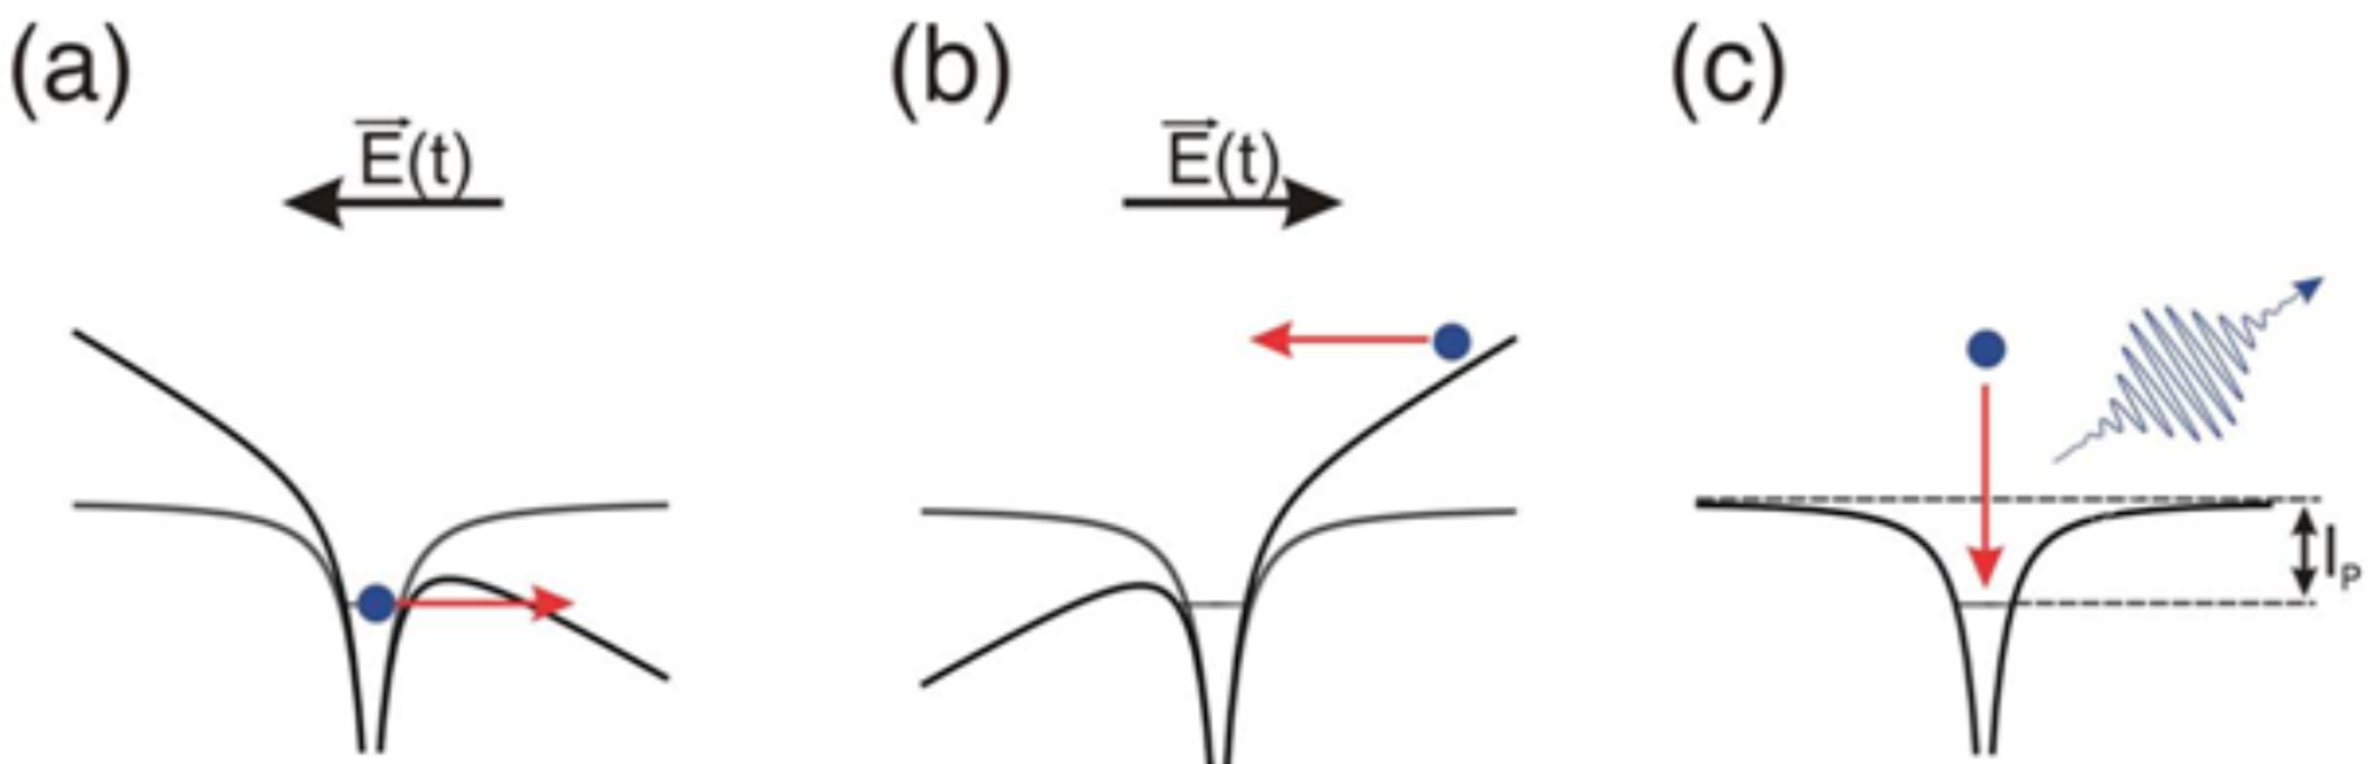
\includegraphics[width=0.9\textwidth]{pic/3step.pdf}
	\caption[Lab coordinate system]{Three step model: (a) Ionization/Tunneling (b) Accelaeration (c) Recombination}
	\label{fig: 3step}
\end{figure}
However, this model is not directly applicable to solid-state HHG due to differences in density, structure, band structure, Coulomb interactions, and surface effects between gases and solids. Solid-state HHG involves more complex mechanisms, including interactions with the crystalline lattice and surface effects, requiring sophisticated theoretical models for accurate description.

The understanding and control of HHG have been greatly advanced by the development of sophisticated
theoretical models, the primary and widely used numerical methods are based on time-dependent
Schrödinger equation (\gls{TDSE}) , semiconductor Bloch equations (\gls{SBE})
and time-dependent density-functional theory (\gls{TDDFT}).
We won't go in detailed about the theoretical foundations, but just summarize current status and some challenges of present numerical simulations which are yet to be improved or solved, for detailed mechanisms and numerical implementations, please refer to the basic references where all those methods are disucssed at lenght.

\begin{itemize}
	\item The time-dependent-Schr\"odinger equation (\gls{TDSE}) model \cite{wu2015high, wu2017orientation, plaja1992high, hawkins2015effect, ndabashimiye2016solid, wu2016multilevel, guan2016high, jin2018high, du2018high}, utilizing both Bloch state basis and Houston state basis, is proficient in examining electronic dynamics within periodic potentials. Nonetheless, simulating the HHG of real solid materials proves challenging, primarily due to the method's reliance on idealized model potentials.
	\item The semiconductor Bloch equations (\gls{SBE}) \cite{hohenleutner2015real, schubert2014sub, langer2016lightwave, vampa2014theoretical, mcdonald2017enhancing, yu2018two, luu2016high, golde2008high, jiang2018role, vampa2015semiclassical, tamaya2016diabatic}, improving it from a two-band model to a multiband model allows for a more comprehensive study of real systems, effectively capturing the main features of High-Order Harmonic Generation (HHG) in solids. This enhancement involves incorporating accurate energy bands and transition dipole moments derived from first-principles calculations. Future endeavors should focus on obtaining the correct phase of transition dipole elements. However, a significant challenge persists as current first-principles codes often yield random phases for transition dipole moments.
	\item The time-dependent density-functional theory (\gls{TDDFT}) model \cite{tancogne2017impact, tancogne2018ultrafast, tancogne2017ellipticity, hansen2017high, meng2018real, floss2018ab, bauer2018high} appears to be the ideal approach for straightforwardly studying High-Order Harmonic Generation (HHG) in solids within real coordinate space. However, its main drawback lies in its significant computational time requirements. Additionally, directly and intuitively analyzing the physical processes or mechanisms within the solid-state energy band picture can pose challenges within the TDDFT framework.
\end{itemize}
Furthermore, properly incorporating Berry curvature in models and understanding its role in solid High-Order Harmonic Generation (HHG) requires more attention in future theoretical simulations. Despite lingering open questions in this evolving field, it's hoped that this review can offer valuable reference points, and ongoing efforts from the relevant community will gradually illuminate the intricacies of solid HHG studies.
%==============================================================================================================================================================================
\section{Structure of the Thesis}
This thesis is organized as follows: Chapter.~\ref{ch:ch2} first introduces the crystallographic discription
for typical hexagonal lattice we are studying, then we study the light-induced electron dynamics in 2D materials based on the tight-binding model by
time-dependent Schrodinger Equation and quantum master equation, to account for dissipative phenomena that plays a fundamental role in the laser induced electron dyanmics that we will describe in detail in the follwoing chapters of this thesis.
In Chapter.~\ref{ch:ch3} we investigate light-induced electron dynamics in monolayer hexagonal
boron nitride under the influence of two-color linearly-polarized laser fields at frequencies
$\omega$ and $2\omega$, by solving the time-dependent Schr\"odinger equation with a tight-binding
model. We start from time-dependent perturbative analysis in the weak field regime, then we expand
our results to third-order nonlinear regime and deeply off-resonant highly-nonlinear regime.
In Chapter.~\ref{ch:ch4}, we study THz-induced HHG in graphene with the method described by quantum
master equation. The microscopic mechanism of
HHG with the quasi-static approximation and the population distribution in the Brillouin zone is
described in detail together with its numerical implementation in Chapter.~\ref{ch:ch5}. We further elucidate the role of the nonequilibrium nature of THz-induced electron dynamics by comparing the nonequilibrium picture in the present work and the thermodynamic picture in the previous work \cite{mics2015thermodynamic}.
We explore the possibility of using a THz
field to enhance MIR-induced HHG in graphene based
on the knowledge gained from Chapter.~\ref{ch:ch4}. We investigate the dynamics under MIR and THz fields and evaluate the emitted harmonic spectra. As a result of the analysis, we find that cou- pling via the induced coherence by THz and MIR fields plays an essential role in enhancing MIR-induced HHG, clarifying the importance of the field-induced coherence beyond the simple population effect.
Finally, the conclusion and perspectvies of this thesis is summarized in in Chapter.~\ref{ch:ch6}

%----------------------------------------------------------------------------------------
% CHAPTER TWO
%----------------------------------------------------------------------------------------
\chapter{THEORETICAL FOUNDATIONS} 
\label{ch:ch2}
%%%%%%%%%%%%%%%%%%%%%%%%%%%%%%%%%%%%%%%%%%%%%%%%%%%%%%%%%%%%%%%%%%%%%%%%%%%%%%%%%%%
\section{Crystallography Properties}
%%%%%%%%%%%%%%%%%%%%%%%%%%%%%%%%%%%%%%%%%%%%%%%%%%%%%%%%%%%%%%%%%%%%%%%%%%%%%%%%%%%
The hexagonal lattice nanostructure, a fundamental Bravais lattice, manifests as a distinctive geometric arrangement prevalent across a spectrum of materials, owing to its highly efficient packing characteristics. This lattice's spatial configuration profoundly influences the mechanical, electrical, and thermal properties of materials. Understanding lattice structures is crucial for deciphering material behavior across diverse conditions, spanning from semimetals to topological insulators. This significance is particularly noteworthy in the realm of two-dimensional materials. We have selected graphene, exemplifying a semimetal, and hexagonal boron nitride (h-BN), recognized as an insulator, for our discussion on nonlinear optical response on 2d materials.\\
\begin{figure}[htpb]
    \centering
    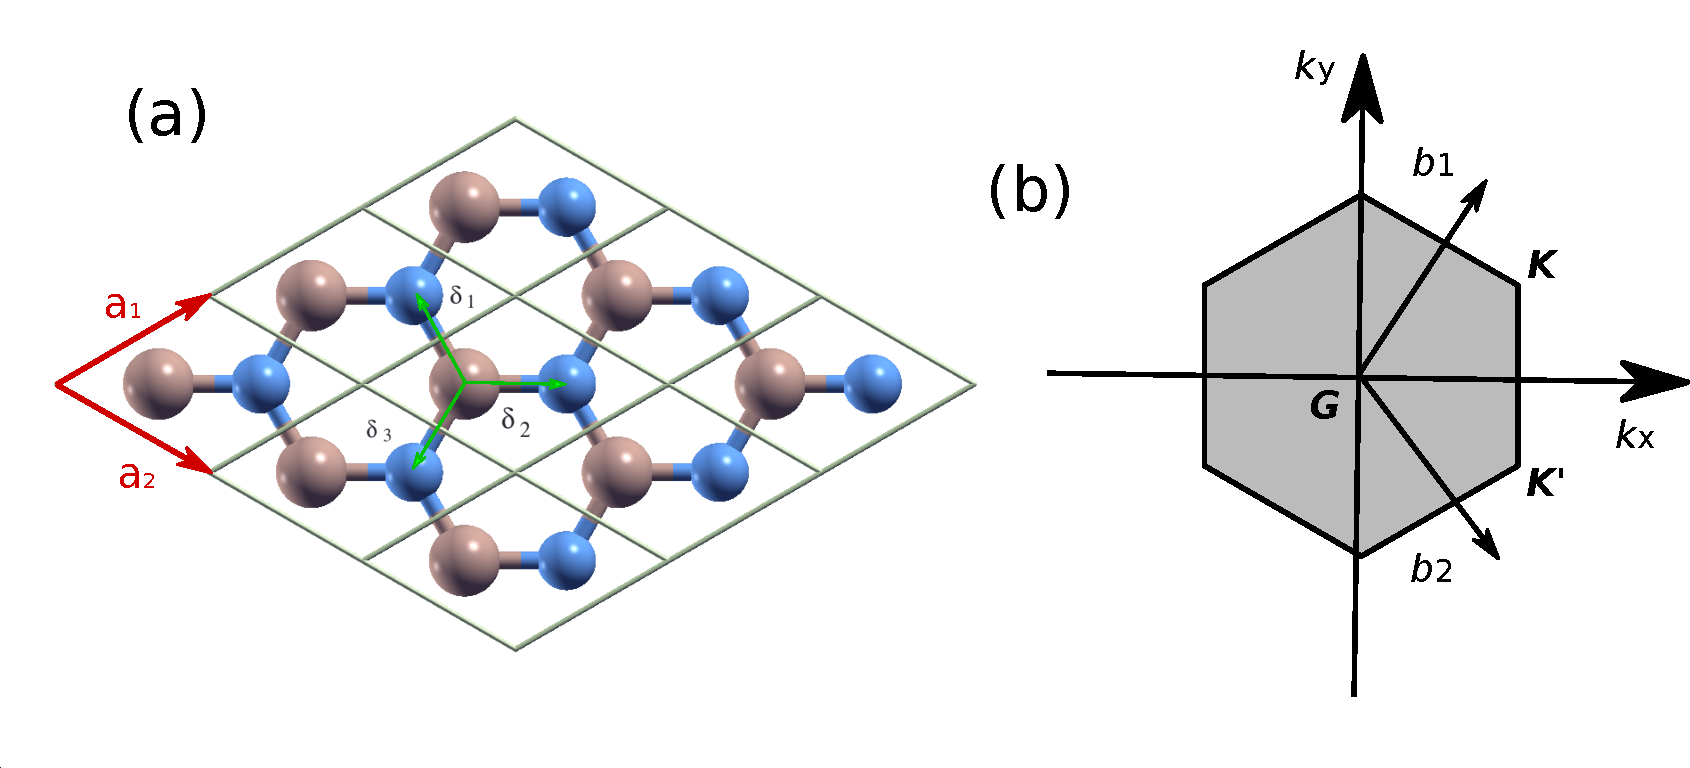
\includegraphics[width=0.96\textwidth]{pic/lattice.pdf}
    \caption[Lab coordinate system]{(a) Hexagonal lattice showing in different colors the two triangular sublattices. (b) Brillouin zone in momentum space.}
    \label{fig: lattice}
\end{figure}
Graphene, an extraordinary carbon allotrope, showcases a captivating atomic arrangement within a hexagonal lattice nanostructure, depicted in Figure \ref{fig: lattice} (a). Carbon atoms meticulously align in a single layer, forming an exceptional two-dimensional material. The unique atomic-scale hexagonal lattice structure involves each carbon atom intricately bonding through $\sigma$-bonds with its three nearest neighbors and a delocalized $\pi$-bond. This precise arrangement plays a pivotal role in the formation of a valence band elegantly spanning the entirety of the graphene sheet, making monolayer graphene an outstanding conductor of electricity, and finding applications in electronic devices, sensors, and various fields.

Similar to graphene, Hexagonal boron nitride (\gls{h-BN}) also features a hexagonal lattice structure, but with alternating boron and nitrogen atoms forming the hexagons, making it a wide-gap insulator due to inversion symmetry breaking, which is used as a dielectric material in electronics, a substrate for graphene-based devices, and as a solid lubricant.
% Example Subsubsection
\subsection{Structural Parameters}
% begin{figure}[tb] % t = top, b = bottom, etc.
 We define the basis of hexagonal lattice primitive vectors $E = (\vec{a}_{1}, \vec{a}_{2})$ as shown in Fig \ref{fig: lattice} (a):
$$
\vec{a}_{1}=a\left(\begin{array}{l}
\frac{\sqrt{3}}{2} \\
\frac{1}{2}
\end{array}\right),
\vec{a}_{2}=a\left(\begin{array}{l}
\frac{\sqrt{3}}{2} \\
-\frac{1}{2}
\end{array}\right)
$$
Where $a$ is the lattice constant, for graphene $a= 1.42 \mathring{A}$ \cite{sarma2011electronic}, and for \gls{h-BN} $a= 2.5 \mathring{A}$ \cite{PhysRevB.81.155433}. Generate only $A$ sites while sites in $B$ sublattice are generated by $n_{1} \vec{a}_{1}+n_{2} \vec{a}_{2}+\vec{\delta},$ where $\vec{\delta}$ has to be chosen as one of the three nearest-neighbor vectors,
$$
\begin{array}{c}
\vec{\delta}_{1}=a\left(\begin{array}{l}
-\frac{1}{2 \sqrt{3}}\\ \frac{1}{2}\end{array}\right), 
\vec{\delta}_{2}=a\left(\begin{array}{l}\frac{1}{\sqrt{3}}\\ 0 \end{array}\right),
\vec{\delta}_{3}=a\left(\begin{array}{l} -\frac{1}{2 \sqrt{3}}\\ -\frac{1}{2}\end{array}\right)
\end{array}
$$
\subsection{Reciprocal Space}
The reciprocal basis $B=\left(b_{1}, b_{2}, b_{3}\right)$ is generated using the formula:
$$
\overrightarrow{b_{k}}=\frac{2 \pi \cdot \overrightarrow{a_{i}} \times \overrightarrow{a_{j}}}{V}
$$
$i, j, k$ are circular permutations, $\mathrm{V}$ the mix product between the three vectors, i.e. the volume of the unitary cell.  Then we get the $2 \mathrm{D}$ reciprocal vectors as shown in Fig\ref{fig: lattice} (b):
$$
\vec b_{1}=k_{D}\left(\begin{array}{l}
\frac{1}{2} \\
\frac{\sqrt{3}}{2} 
\end{array}\right),
\vec b_{2}=k_{D}\left(\begin{array}{c}
\frac{1}{2} \\
-\frac{\sqrt{3}}{2} 
\end{array}\right)
$$
And with $k_{D}=\frac{4 \pi}{\sqrt{3} a}$. The corresponding Brillouin zone is depicted together with the two high-symmetry points $\mathrm{K}$ and $\mathrm{K'}$ Fig ~\ref{fig: lattice} (b).
Two inequivalent corners of the Brillouin zone $K$ and $K^{\prime}$ can be chosen as follows:
$$
K=k_{D}\left(\frac{1}{2}, \frac{1}{2 \sqrt{3}}\right), \quad K^{\prime}=k_{D}\left(\frac{1}{2},-\frac{1}{2 \sqrt{3}}\right)
$$

%%%%%%%%%%%%%%%%%%%%%%%%%%%%%%%%%%%%%%%%%%%%%%%%%%%%%%%%%%%%%%%%%%%%%%%%%%%%%%%%%%%
\section{Tight-binding Approach \label{sec:tightbinding}}
%%%%%%%%%%%%%%%%%%%%%%%%%%%%%%%%%%%%%%%%%%%%%%%%%%%%%%%%%%%%%%%%%%%%%%%%%%%%%%%%%%%

In this section, we delve into the fundamental principles of the tight-binding approach, with a particular focus on the nearest neighbor tight-binding model. This approach is essential for understanding the electronic properties of materials and is a crucial component of graphene's electronic structure analysis.

The foundation of the tight-binding approach is rooted in the Bloch theorem, which is satisfied by the tight-binding function
\begin{equation}
\Phi_{\alpha}(\mathbf{r}, \mathbf{k})=\frac{1}{\sqrt{N}} \sum_{\mathbf{R}} e^{i \mathbf{k} \cdot \mathbf{R}} \phi_{\alpha}\left(\mathbf{r}-\mathbf{R}_{\alpha}\right), \alpha=A \text { or } B
\label{eqn:Bloch}
\end{equation}
Here, $N$ represents the number of unit cells, and $\phi_{\alpha}(\mathbf{r} - \mathbf{R}_{\alpha})$ denotes the orbital function of an electron at cell $\mathbf{R}$ in sublattice $\alpha$.
In the context of a honeycomb lattice, we focus on the nearest neighbor approximation. This approximation asserts that an atom in sublattice A only interacts with its three closest neighbor atoms in sublattice B. This simplification is particularly useful for understanding the interactions between electrons bound to non-equivalent atoms.

The Hamiltonian operator for this nearest-neighbor interaction is expressed as:
\begin{align}
\hat{H}_{A B}=\frac{1}{N} \sum_{\mathbf{R}_{A}} \sum_{\mathbf{R}_{B}} e^{i \mathbf{k}\left(\mathbf{R}_{B}-\mathbf{R}_{A}\right)}\left\langle\phi_{A}\left(\mathbf{r}-\mathbf{R}_{\mathbf{A}}\right)|\hat H| \phi_{B}\left(\mathbf{r}-\mathbf{R}_{B}\right)\right\rangle
\end{align}
Due to the translational invariance in a Bravais lattice, the summation over each atom in a sublattice occurs $N$ times, simplifying the expression to:
\begin{align}
\hat{H}_{A B}=\sum_{\mathbf{R}_{A}} e^{i \mathbf{k}\left(\mathbf{R}_{B}-\mathbf{R}_{A}\right)}\left\langle\phi_{A}\left(\mathbf{r}-\mathbf{R}_{\mathbf{A}}\right)|\hat{H}| \phi_{B}\left(\mathbf{r}-\mathbf{R}_{B}\right)\right\rangle
\end{align}
To transition from real space to momentum space, we employ a Fourier transform, allowing us to represent the Hamiltonian in terms of momentum space. This transformation results in the tight-binding Hamiltonian under the momentum representation, as defined by:
\begin{align}
c_{ \mathbf{R}_{\alpha}, \sigma}=\frac{1}{\sqrt{N}} \sum_{\mathbf{k}} e^{i \mathbf{k} \cdot 
 \mathbf{R}_{\alpha}} c_{\mathbf{k}, \sigma} \\
 c_{\mathbf{R}_{\alpha}, \sigma}^{\dagger}=\frac{1}{\sqrt{N}} \sum_{\mathbf{k}} e^{-i \mathbf{k} \cdot \mathbf{R}_{\alpha}} c_{\mathbf{k}, \sigma}^{+}
 \label{eqn: FT}
\end{align}
 $\sigma=\uparrow, \downarrow$ presents the electron spin,
 With the  orthogonal normalization conditions 
 \begin{align}
   \delta_{\mathrm{kk}^{\prime}}=\frac{1}{N} \sum e^{i\left(k-k^{\prime}\right) \cdot \mathrm{R}_{\alpha}}  
 \end{align}
 We transform the Hamiltonian of real space into the momentum space representation, and then the tight-binding Hamiltonian under the momentum representation is:
\begin{equation}
\hat{H} =\left(\begin{array}{cc}
\epsilon_{A} & t_{0} f(\mathbf{k}) \\
t_{0} f(\mathbf{k})^{*} & \epsilon_{B}
\end{array}\right)
\label{eqn: TBh}
\end{equation}

Here $\epsilon_{A}$ and $\epsilon_{B}$ are the on-site energies of electrons on the nearest neighbor atoms, $t_0$ presents the hopping parameter:
$$
t_{0}=\left\langle\phi_{A}\left(\mathbf{r}-\mathbf{R}_{\mathbf{A}}\right)|\hat{H}| \phi_{B}\left(\mathbf{r}-\mathbf{R}_{A}-\vec{\delta}_{i}\right)\right\rangle \quad(i=1,2,3)
$$\\
For graphene, we set $\epsilon_{A}$ and $\epsilon_{B}$ to 0, and $t_0=2.8~eV$ in accordance with the previous work  \cite{sarma2011electronic}. For h-BN $\epsilon_{\mathrm{B}}$ and $\epsilon_{\mathrm{N}}$ denote the on-site energies for boron and nitrogen sites, respectively. 
\begin{equation}
\hat{H}(\mathbf{k})=\left(\begin{array}{cc}
\epsilon_{\mathrm{B}} & t_{0} f(\mathbf{k}) \\
t_{0} f(\mathbf{k})^{*} & \epsilon_{\mathrm{N}}
\end{array}\right),
\label{eqn:hBNhamiltonian}
\end{equation}
We set $\epsilon_{\mathrm{B}}$ to $3.34$~eV and $\epsilon_{\mathrm{N}}$ to $-2.56~eV$ and $t0$ to $2.6~eV$ computed with the first-principles calculations~\cite{PhysRevB.51.6868}, the band gap $E_{g}=\epsilon_{b}-\epsilon_{n}$ equals 5.9~eV. 

The off-diagonal terms of the tight-binding Hamiltonian \ref{eqn: TBh}:
\begin{equation}
 \begin{aligned}
f(\mathbf{k}) &=e^{i \mathbf{k} \vec{\delta}_{1}}+e^{i \mathbf{k} \vec{\delta}_{2}}+e^{i \mathbf{k} \vec{\delta}_{3}} \\
&=e^{-\frac{i a k_{x}}{\sqrt{3}}}+2 e^{\frac{i a k_{x}}{2 \sqrt{3}}} \cos \left(\frac{a}{2} k_{y}\right)
\end{aligned}
\label{eqn:nearest_h}
\end{equation}
Solving the stationary Schrödinger equation using matrix diagonalization:
\begin{align}
\hat{H}_{\vecb{k}}|\phi_{b \vecb{k}}\rangle = \epsilon_{b\vecb{k}}|\phi_{b}\rangle,
\label{eq:eqigenstates-h0}
\end{align}
We get the eigenenergy of Hamiltonian from \ref{eqn: TBh}, where $b$ is a band index, $|\phi_{b\vecb{k}}\rangle$ is an eigenstate, and $\epsilon_{b\vecb{k}}$ corresponds to the eigenenergy. As the Hamiltonian is a $2$-by-$2$ matrix in this work, the band index $b$ denotes either a conduction ($b=c$) or valence ($b=v$) state.

\begin{equation}
\epsilon_{b\vecb{k}}=E_{0} \pm \frac{1}{2} \sqrt{E_{g}^{2}+4t_{0}^{2}|f|^{2}}
\label{eigenvalues}
\end{equation}
$E_{0}=\frac{\epsilon_{A}+\epsilon_{B}}{2}$ and $E_{g}=\epsilon_{b}-\epsilon_{n}$ is the energy gap. For graphene, $\epsilon_{A} = \epsilon_{B} =0$ the band gap equals 0.
Their corresponding eigenvectors are:
\begin{equation}
    |\phi_{b}\rangle  =\left(\begin{array}{cc}
 \frac{E_{g} \pm \sqrt{E_{g}^{2}+4t_{0}^{2}|f|^{2}}}{2t_{0} f^*}\\
1
\end{array}\right)
\label{eqn:eigenvector}
\end{equation}

%%%%%%%%%%%%%%%%%%%%%%%%%%%%%%%%%%%%%%%%%%%%%%%%%%%%%%%%%%%%%%%%%%%%%%%%%%%%%%%%%%%
\section{Electron Dynamics}
%%%%%%%%%%%%%%%%%%%%%%%%%%%%%%%%%%%%%%%%%%%%%%%%%%%%%%%%%%%%%%%%%%%%%%%%%%%%%%%%%%%
Consider the crystal under the electric field $\vecb {E}$, to avoid that
Bloch’s theorem cannot be applied, let the electric field enter through a uniform vector potential $\vecb {A} (t)$. The time-dependent Hamiltonian is written as
\begin{align}
\hat{H}(t)=\frac{[\hat{\boldsymbol{p}}+e \boldsymbol{A}(t)]^{2}}{2 m}+V(\boldsymbol{r})
\end{align}
Transforming to the $\boldsymbol{k}$ -space representation, we have
\begin{equation}
     \hat{H}(\boldsymbol{k}, t)=\hat{H}\left(\boldsymbol{k}+\frac{e}{\hbar} \boldsymbol{A}(t)\right)
     \label{eqn:vTD}
\end{equation}
where $\boldsymbol k$ denotes the Bloch wavevector, and $|\psi_{\boldsymbol k}(t)\rangle$ is a single-particle electroinc wavefunction at $\boldsymbol k$. The vector potential $\vecb A(t)$ is related to the applied electric field $\vecb E(t)$ as $\vecb E(t)=-d\vecb A(t)/dt$, and it is included in the Hamiltonian as the wavevector shift $\boldsymbol k \rightarrow \boldsymbol k + e\vecb A(t)/\hbar$ via the Peierls substitution  \cite{hofstadter1976energy}.\\
%===================================================================================================================================
\subsection{Time-dependent Schr\"odinger Equation}
The light-induced electron dynamics can be described by solving the following time-dependent Schr\"odinger equation (\gls {TDSE}) at each $\vecb k$-point:
\begin{equation}
i\hbar \frac{d}{dt}| \psi_{\boldsymbol {k}}(t) \rangle = \hat{H}\left ( \boldsymbol k + \frac{e\vecb A(t)}{\hbar} \right )| \psi_{\boldsymbol k}(t) \rangle,
\label{eqn:TDSE}
\end{equation}
Solving this time-dependent Schr\"odinger equation (\gls {TDSE}) is an initial value problem. In two-band systems, usually the ground state $\psi_{\boldsymbol k}(0)$ is used as the initial state occupied at the valence band with:
\begin{align}
\psi_{\boldsymbol k}(0) = \left(\begin{array}{cc}
0 \\
1
\end{array}\right)
\end{align}
The adiabatic approximation is used almost all the time in solving time-propagation, which will be explained in more detail in the appendix \ref{sec:A_ADIABATIC}. Various numerical schemes can be chosen for doing the time propagation, here we split the propagation into short-time propagation using the composition property:
\begin{equation}
\left|\psi_{\boldsymbol{k}}(t')\right\rangle=\exp \left[-i \int_{t}^{t'} d \tau \hat{H}(\tau) \right]\left|\psi_{\boldsymbol{k}+\vecb{A}(t)}\right\rangle
\label{eqn:Houston}
\end{equation}
In practice, simpler schemes are usually used and self-consistency is often neglected. Instead, we rely on a sufficiently small $\Delta t$, $t'=t+\Delta t$, the exponential mid-point propagator is given by:
\begin{align}
    U(t+\Delta t, t) \approx U_{E M}(t+\Delta t, t)=\exp \{-\mathrm{i} \Delta t \hat{H}(t+\Delta t / 2)\}
\end{align}
We approximate the exponential using a Taylor expansion to fourth-order:
\begin{align}
    \exp \{A\}=\sum_{k=0}^{\infty} \frac{1}{k!} A^k
\end{align}
Once the time-evolution of the wavefunctions, $|\psi_{\vecb k}(t)\rangle$ is computed, the current induced in the matter can be further evaluated with
\begin{align}
\vecb{J}_{\vecb k}(t)=\frac{1}{(2\pi)^2} \int_{BZ} d\vecb k\langle \psi_{\vecb k}(t)|\hat{\vecb J}_{\vecb k}(t)| \psi_{\vecb{k}}(t)\rangle.
\label{eq:current}
\end{align}
Here, $\hat {\vecb J}_{\vecb k}(t)$ is the current operator, and it is defined as
\begin{align}
\hat {\vecb J}_{\vecb k}(t) = \frac{\partial }{\partial \vecb k}\hat H \left (\vecb k + \frac{e\vecb A(t)}{\hbar} \right ) = 
-t_0 \left(\begin{array}{cc}
0 & \frac{\partial f(\boldsymbol{k}+\boldsymbol{A})}{\partial \boldsymbol A} \\
\frac{\partial f^*(\boldsymbol{k}+\boldsymbol{A})}{\partial \boldsymbol A}  & 0
\end{array}\right),
\end{align}

where $\frac{\partial f(\vecb k)}{\partial \vecb k}$ is given by 
\begin{align}
\frac{\partial f(\vecb k)}{\partial \vecb k}=i \vecb{\delta}_1e^{i\vecb k \cdot \vecb \delta_1}
+i \vecb{\delta}_2e^{i\vecb k \cdot \vecb \delta_2}
+i \vecb{\delta}_3e^{i\vecb k \cdot \vecb \delta_3}.
\end{align}
Current \ref{eq:current} can be further decomposed into:
\begin{equation}
\begin{array}{l}
\boldsymbol{J}_{b,k}(t)=\left\langle \psi_{b, \boldsymbol{k}}(t)|\boldsymbol{J}(t))| \psi_{b, \boldsymbol{k}}(t)\right\rangle \\
=\sum\limits_{b',b''} c_{b^{\prime} \boldsymbol{k}}(t) c_{b^{\prime \prime} \boldsymbol{k}}^{*}(t)\left\langle \phi_{b^{\prime \prime} \boldsymbol{k}}^{H}(t)|\boldsymbol{J}(t))| \phi_{b^{\prime} \boldsymbol{k}}^{H}(t)\right\rangle+\sum\limits_{b',b''}\left|c_{b^{\prime} k}(t)\right|^{2}\left\langle \phi_{b^{\prime} k}^{H}(t)|\boldsymbol{J}(t))| \phi_{b^{\prime} k}^{H}(t)\right\rangle
\end{array}
    \label{totalcurrent}
\end{equation}
Here the off-diagonal terms contribute to the Interband current, and the diagonal terms contribute to the Intraband current. \\
\begin{equation}
\begin{array}{l}
\boldsymbol{J}_{inter;b,k}(t)=\sum\limits_{b',b''} c_{b^{\prime} \boldsymbol{k}}(t) c_{b^{\prime \prime} \boldsymbol{k}}^{*}(t)\left\langle \phi_{b^{\prime \prime} \boldsymbol{k}}^{H}(t)|\boldsymbol{J}(t))| \phi_{b^{\prime} \boldsymbol{k}}^{H}(t)\right\rangle
\end{array}
    \label{intercurrent}
\end{equation}

\begin{equation}
\begin{array}{l}
\boldsymbol{J}_{intra;b,k}(t)=\sum\limits_{b',b''}\left|c_{b^{\prime} k}(t)\right|^{2}\left\langle \phi_{b^{\prime} k}^{H}(t)|\boldsymbol{J}(t))| \phi_{b^{\prime} k}^{H}(t)\right\rangle
\end{array}
    \label{intracurrent}
\end{equation}
By combining time-dependent wavefunction $\psi_{\vecb{k}}(t)$ solved from Eq.~(\ref{eqn: TBh}) and the eigenstates $\phi_{c\vecb{k}}$ defined with Eq.~(\ref{eq:eqigenstates-h0}), the conduction population distribution $n_{c \vecb{k}}$ with the laser irradiation at instantaneous time $t$  can be evaluated as:
\begin{equation}
  n_{c\vecb{k}} = \left | \langle \phi_{c\vecb{k}} | \psi_{\vecb{k}}(t) \right |^2,
  \label{eq:population_tdse}
\end{equation}
$\frac{\partial\epsilon_{b,\boldsymbol{k}+\boldsymbol{A}(t)}}{\partial\boldsymbol{k}} = -\left\langle \phi_{b^{\prime} k}^{H}(t)|\boldsymbol{J}(t))| \phi_{b^{\prime} k}^{H}(t)\right\rangle$ defines the band velocity. The eigenenergy of conduction band at time $t$ is $\epsilon_{c,\boldsymbol{k}+\boldsymbol{A}(t)}=E_{0} + \frac{1}{2} \sqrt{E_{g}^{2}+4t_{0}^{2}|f(\boldsymbol{k}+\boldsymbol{A}(t))|^{2}}$\\

\begin{equation}
    \frac{\partial\epsilon_{v,\boldsymbol{k}+\boldsymbol{A}(t)}}{\partial\boldsymbol{k}}=-\frac{t_0^2}{2\epsilon_{v,k+\boldsymbol{A}(t)}-(\epsilon_b+\epsilon_n)}\cdot (f^*(\boldsymbol{k}+\boldsymbol{A}(t))\frac{\partial f(\boldsymbol{k}+\boldsymbol{A}(t))}{\partial k}+c.c.)
    \label{band velocity_v}
\end{equation}

\begin{equation}
    \frac{\partial\epsilon_{c,\boldsymbol{k}+\boldsymbol{A}(t)}}{\partial\boldsymbol{k}}=\frac{t_0^2}{2\epsilon_{c,k+\boldsymbol{A}(t)}-(\epsilon_b+\epsilon_n)}\cdot (f^*(\boldsymbol{k}+\boldsymbol{A}(t))\frac{\partial f(\boldsymbol{k}+\boldsymbol{A}(t))}{\partial k}+c.c.)
    \label{band velocity_c}
\end{equation}
%==================================================================================================================================
\subsection{Quantum Master Equation \label{sec:master}}
In contrast to closed quantum systems, which are entirely isolated from external influences and can be adequately described by the Schrödinger equation, the quantum master equation is typically used in the context of the time evolution of an open quantum system, where the system of interest is susceptible to exchanges of energy, particles, or information with its external environment. 
To expound processes such as relaxation, dephasing, and thermalization of the nonlinear response experiments, the quantum master equation is predominantly employed which is salient in the realm of open quantum systems.\\
We describe the light-induced electron dynamics in graphene with the following quantum master equation \cite{sato2019light,sato2019microscopic,sato2021high,sato2021nonlinear}:
\begin{equation}
\frac{\mathrm{d}}{\mathrm{d}t}\rho_{\boldsymbol{k}}(t) = \frac{1}{i \hbar}	\left[ \hat{H}_{\boldsymbol{k}+e\boldsymbol{A}(t)/\hbar}, \rho_{\boldsymbol{k}} (t)) \right] + 	
\hat{D}\left[ \rho_{\boldsymbol{k}} (t)) \right],
\label{eqn:masterequation}
\end{equation}
$\rho_{\vecb k}(t)$ is the reduced density matrix at $\vecb k$. The quantum master equation delineates the dynamical evolution of the density matrix associated with the quantum system, which encompasses both pure and mixed quantum states. 
To elucidate the impact of dissipation, we formulate the relaxation operator, denoted as $\hat{D}\left[\rho_{\vecb{k}} (t)\right]$, within the framework of Eq.(\ref{eqn:masterequation}) employing the relaxation time approximation\cite{meier1994coherent} and employing the Houston basis \cite{PhysRev.57.184, PhysRevB.33.5494}. The Houston states are characterized as eigenstates of the instantaneous Hamiltonian, expressed as:
\begin{align}
\hat{H}_{\vecb{k}+e\vecb{A}(t)/\hbar} |u^H_{b\vecb k}(t)\rangle = \epsilon_{b,\vecb k + e\vecb A(t)/\hbar}|u^H_{b\vecb k}(t)\rangle   
\label{eqn:Houston}
\end{align}
The expansion of the reduced density matrix can then be carried out using the Houston states.
\begin{align}
  \rho_{\vecb k}(t) = \sum_{bb'}\rho_{bb',\vecb k}(t)|u^H_{b\vecb k}(t)\rangle \langle u^H_{b'\vecb k}(t)|,
\end{align}
where $\rho_{bb',\vecb k}(t)$ are the expansion coefficients. On the basis of the Houston state expansion, we define the relaxation operator \cite{sato2019microscopic,PhysRevB.99.214302,sato2019light} as
\begin{align}
    \hat D\left [\rho_{\vecb k}(t) \right ]=&-\sum_{b}\frac{\rho_{bb,\vecb k}(t)-f^{FD}\left
(\epsilon_{b,\vecb k+e\vecb A(t)/\hbar},T_e,\mu \right)}{T_1}|u^H_{b\vecb k}(t)\rangle \langle
u^H_{b\vecb k}(t)|\\ 
                                            &-\sum_{b\neq b'} \frac{\rho_{bb',\vecb k}(t)}{T_2}|u^H_{b\vecb k}(t)\rangle \langle u^H_{b'\vecb k}(t)|,
\label{eqn:relaxation}
\end{align}
$T_1$ is the longitudinal relaxation time, $T_2$ is the transverse relaxation time, and $f^{\mathrm{FD}}(\epsilon)$ is the Fermi--Dirac distribution
\begin{align}
f^{\mathrm{FD}}(\epsilon, T_e, \mu)=\frac{1}{e^{(\epsilon-\mu)/k_BT_e}+1}.
\label{eq:fd-dist}
\end{align}
$\mu$ is the chemical potential, and $T_e$ is the electron temperature.
In the following discussion, we set the longitudinal relaxation time $T_1$ to $100$~fs and the transverse relaxation time $T_2$ to $20$~fs in accordance with the previous works \cite{sato2021nonlinear,sato2021high,sato2019light,sato2019microscopic}. The electron temperature $T_e$ is set to $300$~K unless stated otherwise. The chemical potential $\mu$ is treated as a tunable parameter to study the effect of doping.\\
We directly solve the quantum master equation, Eq.~(\ref{eqn:masterequation}), in the time domain by employing the Runge-Kutta method without any approximation.
The electric current is obtained by employing the time-dependent density matrix $\rho_{\vecb k}(t)$, which evolves according to Eq.~(\ref{eqn:masterequation}):
\begin{eqnarray}
  \vecb{J}(t)=\frac{2}{(2\pi)^2} \int d\vecb k \mathrm{Tr}\left[\hat{\boldsymbol{J}}_{\boldsymbol{k}}(t)\rho_{\boldsymbol{k}}(t)\right],
\label{eqn:totalcurrent}
\end{eqnarray}
where $\hat{\boldsymbol{J}}_{\boldsymbol{k}}(t)$ is the current operator defined as
\begin{align}
\hat{\boldsymbol J}_{\boldsymbol{k}}(t) = -\frac{\partial H(\boldsymbol{k}+e\boldsymbol{A}(t)/\hbar)}{\partial \boldsymbol A(t)}.
\label{totalcurrent}
\end{align}
The intraband component of the current is
\begin{align}
\boldsymbol{J}^{\mathrm{intra}}_{\vecb k}(t)&=\sum_{b=v,c} \frac{(-2)}{(2\pi)^2}
\frac{e}{\hbar} \nonumber \times  
\int d\boldsymbol{k}\frac{\partial\epsilon_{b,\boldsymbol{k}+e\boldsymbol{A}(t)/\hbar}}{\partial\boldsymbol{k}} n_{b,\boldsymbol{k}+e\boldsymbol{A}(t)/\hbar},
\label{eqn:intra-steady-current}
\end{align}
where the band population $n_{b,\boldsymbol{k}+e\boldsymbol{A}(t)/\hbar}$ is defined with the Houston states of the Hamiltonian $|u^H_{b,\boldsymbol k} (t)\rangle$ computed from Eq ~\ref{eqn:Houston}:
\begin{align}
n_{b,\boldsymbol{k}+e\boldsymbol{A}(t)/\hbar}(t)=\langle u^H_{b,\boldsymbol k}(t) |\rho_{\boldsymbol{k}}(t)|u^H_{b,\boldsymbol k}(t) \rangle
\end{align}
%=====================================================================================================================================================



\chapter{CO-LINEAR POLARIZATION INDUCED PHOTOVOLTAIC EFFECT} 
Addressing the photovoltaic effect within the perturbative regime has garnered significant attention, particularly in the exploration of dc current injection using two-color linearly polarized light~\cite{PhysRevLett.74.3596,PhysRevLett.76.1703,PhysRevLett.78.306,Sun2010,PhysRevB.100.075202,HeideBoolakeeEcksteinHommelhoff+2021+3701+3707,PhysRevLett.123.067402}. Early investigations have underscored the intricate interplay between a fundamental frequency, denoted as $\omega$, and its second harmonic, $2\omega$~\cite{PhysRevLett.74.3596,PhysRevLett.76.1703,PhysRevLett.78.306}. 
A notable study by Jimenez-Galan et al.~\cite{Jimenez-Galan2020} utilized deeply off-resonant bi-circular laser fields with frequencies $\omega$ and $2\omega$ to generate a substantial population imbalance in the Brillouin zone. However, it is worth noting that, in principle, the use of linearly polarized light with two frequencies is sufficient to break time-reversal symmetry.

In this Chapter, we first theoretically explore the phenomenon of dc-current injection and the generation of population imbalance through the application of two-color linearly polarized laser fields with frequencies $\omega$ and $2\omega$ based on time-dependent perturbation analysis. To ground our analysis, we scrutinize light-induced electron dynamics in a prototypical two-dimensional material, monolayer hexagonal boron-nitride ($h$-BN), leveraging a simple tight-binding approximation first in a perturbative resonant regime.

In our quantum dynamics simulations, we further uncover that ballistic current can be induced even in the deeply off-resonant regime with two-color linearly polarized light.  Consequently, efficient injection of dc-current and the creation of a substantial population imbalance can be realized by employing two-color linearly polarized laser fields with frequencies $\omega$ and $2\omega$, without relying on the ellipticity of light. These findings offer a potential pathway for achieving ultrafast and efficient control of electron population in matter using multi-color linearly polarized light, opening new avenues for exploring the frontiers of quantum dynamics and optoelectronic applications. This streamlined approach offers a promising avenue for achieving efficient and controlled current injection under conditions of deep off-resonance, potentially opening up new possibilities for nonlinear optoelectronic applications.

%%%%%%%%%%%%%%%%%%%%%%%%%%%%%%%%%%%%%%%%%%%%%%%%%%%%%%%%%%%%%
\section{Time-dependrnt Perturbative Analysis on QuI \label{sec:deriveperturbation}}
%%%%%%%%%%%%%%%%%%%%%%%%%%%%%%%%%%%%%%%%%%%%%%%%%%%%%%%%%%%%%%%
Time-dependent perturbation theory provides a formalism for describing the response of quantum systems to time-varying external fields, making it well-suited for analyzing the interaction of materials with intense electromagnetic radiation. It provides a formalism for describing the response of quantum systems to time-varying external fields, making it well-suited for analyzing the interaction of materials with intense electromagnetic radiation. 
Exploring the photovoltaic effect within the perturbative regime has led to a notable focus on elucidating the injection of direct current (dc) through the use of two-color linearly polarized light ~\cite{PhysRevLett.74.3596,PhysRevLett.76.1703,PhysRevLett.78.306,Sun2010,PhysRevB.100.075202,HeideBoolakeeEcksteinHommelhoff+2021+3701+3707,PhysRevLett.123.067402}. 
Here, we investigate the nonlinear photocarrier injection process via the time-dependent perturbation analysis.
Under adiabatic basis representation described in Appendix ~\ref{ch:Adiabatic}, one can rewrite the equation of motion for the coefficient vector as
\begin{align}
&i\frac{d}{dt} \vecb c_{\vecb k}(t) = 
 \nonumber \\
& i\vecb E(t)\cdot \left(
    \begin{array}{cc}
      0 & 
      e^{-i\int^t_0dt' \Delta \epsilon_{cv,\vecb k+ \vecb A(t')}+i \Delta \phi^g_{cv,\vecb k}(t)} 
  \left \langle u_{v,\vecb k+\vecb A(t)}\Big |\frac{\partial u_{c,\vecb k+\vecb A(t)}}{\partial \vecb k} \right \rangle \\
      e^{-i\int^t_0dt' \Delta \epsilon_{vc,\vecb k+ \vecb A(t')}+i \Delta \phi^g_{vc,\vecb k}(t)} 
  \left \langle u_{c,\vecb k+\vecb A(t)}\Big |\frac{\partial u_{v,\vecb k+\vecb A(t)}}{\partial \vecb k} \right \rangle &
      0
    \end{array}
    \right) \vecb c_{\vecb k}(t) \nonumber \\
&= \mathcal{H}(t) \vecb c_{\vecb k}(t)
.
\label{eq:tdse-ad-basis}
\end{align}

$\vecb c_{\vecb k}(t) = \left(
    \begin{array}{cc}
      c_{v,\vecb k}(t) \\
      c_{c,\vecb k}(t)
    \end{array}
    \right)$ is the coefficient vector,  $\Delta\epsilon_{bb',\vecb k+ \vecb A(t)}$ is defined by the difference of the single-particle energies as $\epsilon_{b,\vecb k+ \vecb A(t)}-\epsilon_{b',\vecb k+ \vecb A(t)}$. For simplicity, here assume that the contributions from the geometric phases, $\Delta \phi^g_{cv,\vecb k}(t)$ are zero. Then expand the Hamiltonian in Eq.~(\ref{eq:tdse-ad-basis}) up to the second order of the field $\vecb A(t)$ as
\begin{align}
\mathcal{H}(t)\approx \mathcal{H}^{(1)}(t) + \mathcal{H}^{(2)}_{dyn}(t) + \mathcal{H}^{(2)}_{dip}(t),
\end{align}

\begin{align}
\mathcal{H}^{(1)}(t) = i \vecb E(t)\cdot 
\left(
    \begin{array}{cc}
      0 & 
      e^{-i \Delta \epsilon_{cv,\vecb k}t} 
  \left \langle u_{v,\vecb k}\Big |\frac{\partial u_{c,\vecb k}}{\partial \vecb k} \right \rangle \\
      e^{-i\Delta \epsilon_{vc,\vecb k}t}
  \left \langle u_{c,\vecb k}\Big |\frac{\partial u_{v,\vecb k}}{\partial \vecb k} \right \rangle &
      0
    \end{array}
    \right),
\end{align}

$\mathcal{H}^{(2)}_{dyn}(t)$ and $\mathcal{H}^{(2)}_{dip}(t)$, are given by
\begin{align}
\mathcal{H}^{(2)}_{dyn}(t) =   \vecb E(t)\cdot 
\left(
    \begin{array}{cc}
      0 & 
      \frac{\partial \Delta \epsilon_{cv,\vecb k}}{\partial \vecb k}\cdot \left ( \int^t_0 dt' \vecb A(t') \right )e^{-i \Delta \epsilon_{cv,\vecb k}t} 
  \left \langle u_{v,\vecb k}\Big |\frac{\partial u_{c,\vecb k}}{\partial \vecb k} \right \rangle \\
  \frac{\partial \Delta \epsilon_{vc,\vecb k}}{\partial \vecb k} \cdot \left ( \int^t_0dt' \vecb A(t')\right )e^{-i\Delta \epsilon_{vc,\vecb k}t}
  \left \langle u_{c,\vecb k}\Big |\frac{\partial u_{v,\vecb k}}{\partial \vecb k} \right \rangle &
      0
    \end{array}
    \right),
\end{align}
and 
\begin{align}
\mathcal{H}^{(2)}_{dip}(t) =  
\left(
    \begin{array}{cc}
      0 & 
      e^{-i \Delta \epsilon_{cv,\vecb k}t} 
      \vecb A(t) \cdot \frac{\partial 
  \left \langle u_{v,\vecb k}\Big |i \vecb E(t)\cdot  \frac{\partial u_{c,\vecb k}}{\partial \vecb k} \right \rangle 
 }{\partial \vecb k} 
\\
      e^{-i\Delta \epsilon_{vc,\vecb k}t}
      \vecb A(t) \cdot \frac{\partial
  \left \langle u_{c,\vecb k}\Big |i \vecb E(t)\cdot \frac{\partial u_{v,\vecb k}}{\partial \vecb k} \right \rangle
}{\partial \vecb k} 
 &
      0
    \end{array}
    \right).
\end{align}
Here, $\mathcal{H}^{(2)}_{dyn}(t)$ originates from the modification of the dynamical phase factor:
\begin{align}
e^{-i\int^t_0dt' \Delta \epsilon_{vc,\vecb k+ \vecb A(t')}}  
\end{align}
while $\mathcal{H}^{(2)}_{dip}(t)$ originates from the modification of the dipole matrix elements:
\begin{align}
i\left \langle u_{v,\vecb k+\vecb A(t)}\Big |\frac{\partial u_{c,\vecb k+\vecb A(t)}}{\partial \vecb k} \right \rangle    
\end{align}
Hereafter, we analyze the photocarrier injection process based on this perturbative expansion of the Hamiltonian. Use perturbation expansion of Eq.~(\ref{eq:tdse-ad-basis}):
\begin{align}
i\frac{\mathrm{d}  }{\mathrm{d} t} (\vecb c^{(0)}_{\vecb k}(t)+\vecb c^{(1)}_{\vecb k}(t)+\vecb c^{(2)}_{\vecb k}(t))=(\mathcal{H}^{(0)}_{\vecb k}+\mathcal{H}^{(1)}_{\vecb k}(t)+\mathcal{H}^{(2)}_{\vecb k}(t)) (\vecb c^{(0)}_{\vecb k}(t)+\vecb c^{(1)}_{\vecb k}(t)+\vecb c^{(2)}_{\vecb k}(t))
\label{perturbative}
\end{align}
Under initial condition $\mathcal{H}^{(0)}_{\vecb k}(t=0)=0$, $\vecb c^{(0)}_{\vecb k}(t=0) = \left(
    \begin{array}{cc}
      1\\
     0
    \end{array}
    \right)$ ,  the first and second-order coefficient vectors for the conduction band can be written as:
\begin{align}
     c^{(1)}_{c,\vecb k}(t) = \left \langle u_{c,\vecb k}\Big |\frac{\partial u_{v,\vecb k}}{\partial \vecb k} \right \rangle \int_0^t dt' e^{-i \Delta \epsilon_{vc,\vecb k}t'} 
      \vecb E_1(t') 
\label{first_P}
\end{align}

\begin{align}
     c^{(2)}_{c,\vecb k,dyn}(t) = \frac{1}{i} \frac{\partial  \Delta \epsilon_{vc,\vecb k}}{\partial \vecb k} \left \langle u_{c,\vecb k}\Big |\frac{\partial u_{v,\vecb k}}{\partial \vecb k} \right \rangle \int_0^t dt' e^{-i \Delta \epsilon_{vc,\vecb k}t'}\vecb E_2(t') \int_0^{t'}  
    dt'' \vecb A_2(t'') 
    \label{second_dyn}
\end{align}

\begin{align}
     c^{(2)}_{c,\vecb k,dip}(t) =  \frac{\partial \left \langle u_{c,\vecb k}\Big |\frac{\partial u_{v,\vecb k}}{\partial \vecb k} \right \rangle}{\partial \vecb k}   \int_0^t dt' e^{-i \Delta \epsilon_{vc,\vecb k}t'}\vecb E_2(t')  \vecb A_2(t') 
    \label{second_dip}
\end{align}
Under two-color linearly polarized light, here we consider the perturbation by the external linearly polarized vector potential for $\vec e$-direction, assuming that the perturbation only exits time between 0 and $T_0$ under the Gaussian distribution:
\begin{align}
f(t)=e^{-\frac{(t-T_0)^2}{2\sigma^2}}    
\end{align}
\begin{align}
   \vecb A_1(t)=A_1 \vec e cos[2w(t-T_0)+\phi]  e^{-\frac{(t-T_0)^2}{2\sigma^2}}, \\
   \vecb A_2(t)=A_2 \vec e cos[w(t-T_0)]  e^{-\frac{(t-T_0)^2}{2\sigma^2}}
   \label{vector}
\end{align}
$w$ is the carrier frequency of the field,  $\vec{e}$ represents a unit vector along the polarization direction of the laser field
We assume $T_0\gg0$ and $\sigma\gg0$ to make the approximation:
\begin{align}
\int_0^t A_2 \vec e cos[w(t-T_0)]  e^{-\frac{(t-T_0)^2}{2\sigma^2}}=\frac{A_2 \vec e}{w} sin[w(t'-T_0)]  e^{-\frac{(t'-T_0)^2}{2\sigma^2}}    
\end{align}
The corresponding external electric field $\vecb E(t)=-d\vecb A(t)/dt$ can be written as the following pulsed form:

\begin{align}
   \vecb E_1(t)=2wA_1 \vec e sin[2w(t-T_0)+\phi]  e^{-\frac{(t-T_0)^2}{2\sigma^2}}, \\
   \vecb E_2(t)=wA_2 \vec e sin[w(t-T_0)]  e^{-\frac{(t-T_0)^2}{2\sigma^2}}
   \label{feild}
\end{align}

Now, let's express this in terms of the first-order coefficient vector is:
\begin{equation}
\begin{aligned}
     c^{(1)}_{c,\vecb k}(t) &= \left \langle u_{c,\vecb k}\Big |\frac{\partial u_{v,\vecb k}}{\partial \vecb k} \right \rangle \int_0^t dt' e^{-i \Delta \epsilon_{vc,\vecb k}t'} 
      2wA_1 \vec e \cdot sin[2w(t'-T_0)+\phi]  e^{-\frac{(t'-T_0)^2}{2\sigma^2}}\\
      &=\frac{A_1 \vec e w}{i} \left \langle u_{c,\vecb k}\Big |\frac{\partial u_{v,\vecb k}}{\partial \vecb k} \right \rangle \int_0^t dt' e^{-i \Delta \epsilon_{vc,\vecb k}t' - \frac{(t'-T_0)^2}{2\sigma^2}} 
      \cdot (e^{i[2w(t'-T_0)+\phi]}-e^{-i[2w(t'-T_0)+\phi]}) 
\end{aligned}
\end{equation}
We consider the population distribution after the laser pulse, so we replace the integra $\int_0^t$ by $\int_\infty^\infty$. Under the Gaussian integral, 
\begin{align}
\int_{-\infty}^{\infty} e^{-x^2} \, dx = \sqrt{\pi}
\end{align}
we get:
\begin{equation}
\begin{aligned}
     c^{(1)}_{c,\vecb k}(t) = \frac{A_1 \vec e w \cdot \sigma \sqrt{2\pi}}{i} \left \langle u_{c,\vecb k}\Big |\frac{\partial u_{v,\vecb k}}{\partial \vecb k} \right \rangle \cdot  e^{-i\Delta \epsilon_{vc,\vecb k} T_0}
    [e^{-\frac{1}{2}(\Delta \epsilon_{vc,\vecb k} - 2w)^2 \sigma^2-i\phi}
    -e^{-\frac{1}{2}(\Delta \epsilon_{vc,\vecb k} + 2w)^2 \sigma^2+i\phi}]
\end{aligned}
\end{equation}
Similarly to the first-order perturbation coefficient vector's derivation, the second-order coefficient $c^{(2)}_{c,\vecb k}(t)$ can be written as:
\begin{equation}
\begin{aligned}
    c^{(2)}_{c,\vecb k,dyn}(t)=\frac{(A_2 \vec e)^2 \cdot \sigma \sqrt{\pi}}{2i} \frac{\partial  \Delta \epsilon_{vc,\vecb k}}{\partial \vecb k} \left \langle u_{c,\vecb k}\Big |\frac{\partial u_{v,\vecb k}}{\partial \vecb k} \right \rangle \cdot e^{-i\Delta \epsilon_{vc,\vecb k} T_0}
    \cdot [e^{-\frac{\sigma^2}{4} \Delta \epsilon_{vc,\vecb k} ^2}-\frac{1}{2}(e^{-\frac{\sigma^2}{4} (\Delta \epsilon_{vc,\vecb k}-2w)^2}+e^{-\frac{\sigma^2}{4} (\Delta \epsilon_{vc,\vecb k}+2w)^2})]
\end{aligned}
\end{equation}

\begin{equation}
\begin{aligned}
    c^{(2)}_{c,\vecb k,dip}(t)=\frac{(A_2 \vec e)^2 w \cdot \sigma \sqrt{\pi}}{4i} \cdot \frac{\partial{\left \langle u_{c,\vecb k}\Big |\frac{\partial u_{v,\vecb k}}{\partial \vecb k} \right \rangle}}{\partial {\vecb k}} \cdot e^{-i\Delta \epsilon_{vc,\vecb k} T_0} [e^{-\frac{\sigma^2}{4} (\Delta \epsilon_{vc,\vecb k}-2w)^2}-e^{-\frac{\sigma^2}{4} (\Delta \epsilon_{vc,\vecb k}+2w)^2})]
\end{aligned}
\end{equation}
This completes the derivation of the population of the conduction band after the laser pulse:
\begin{equation}
\begin{aligned}
|c_{c,\vecb k}(t)|^2&=|c^{(1)}_{c,\vecb k}(t)|^2+|c^{(2)}_{c,\vecb k,dyn}(t)|^2+|c^{(2)}_{c,\vecb k,dip}(t)|^2\\
    &+ c^{(1)}_{c,\vecb k}(t)^* c^{(2)}_{c,\vecb k,dyn}(t) +c.c.\\
    &+c^{(1)}_{c,\vecb k}(t)^* c^{(2)}_{c,\vecb k,dip}(t)+c.c.\\
    &+c^{(2)}_{c,\vecb k,dyn}(t)^* c^{(2)}_{c,\vecb k,dip}(t)+c.c.
\end{aligned}
\end{equation}
We consider a prototypical two-dimensional insulator, monolayer hexagonal boron-nitride ($h$-BN). For the 2-band hBN-tight-binding model, the inversion symmetric is breaking:
\begin{align}
u_{\vecb k}(-\vec r)\neq u_{-\vecb k}(\vec r)    
\end{align}
We apply the time-reversal relation for the derivation:
\begin{align}
u^*_{\vecb k}(\vec r)= u_{-\vecb k}(\vec r)   
\end{align}
To compare the $|c_{c,-\vecb k}(t)|^2$, the absolute value of the coefficient becomes:

\begin{equation}
\begin{aligned}
  |c^{(1)}_{c,\vecb k}(t)|^2 &=  \lvert \frac{A_1 \vec e w \cdot \sigma \sqrt{2\pi}}{i} \left \langle u_{c,\vecb k}\Big |\frac{\partial u_{v,\vecb k}}{\partial \vecb k} \right \rangle \rvert^2 \\
 & \cdot [e^{-(\Delta \epsilon_{vc,\vecb k} - 2w)^2 \sigma^2}
    +e^{-(\Delta \epsilon_{vc,\vecb k} + 2w)^2 \sigma^2}
    -2e^{-\frac{1}{2}((\Delta \epsilon_{vc,\vecb k} - 2w)^2 \sigma^2
    +(\Delta \epsilon_{vc,\vecb k} + 2w)^2 \sigma^2)}cos(2\phi)]\\
    &=  |c^{(1)}_{c,-\vecb k}(t)|^2
\end{aligned}
\end{equation}

\begin{equation}
\begin{aligned}
  |c^{(2)}_{c,\vecb k,dyn}(t)|^2&= \lvert \frac{(A_2 \vec e)^2 \cdot \sigma \sqrt{\pi}}{2} \frac{\partial  \Delta \epsilon_{vc,\vecb k}}{\partial \vecb k} \left \langle u_{c,\vecb k}\Big |\frac{\partial u_{v,\vecb k}}{\partial \vecb k} \right \rangle 
    \cdot [e^{-\frac{\sigma^2}{4} \Delta \epsilon_{vc,\vecb k} ^2}-\frac{1}{2}(e^{-\frac{\sigma^2}{4} (\Delta \epsilon_{vc,\vecb k}-2w)^2}+e^{-\frac{\sigma^2}{4} (\Delta \epsilon_{vc,\vecb k}+2w)^2})] \rvert^2\\
    &=|c^{(2)}_{c,-\vecb k,dyn}(t)|^2
\end{aligned}
\end{equation}

\begin{equation}
\begin{aligned}
  |c^{(2)}_{c,\vecb k,dip}(t)|^2&= \lvert \frac{(A_2 \vec e)^2 w \cdot \sigma \sqrt{\pi}}{4} \cdot \frac{\partial{\left \langle u_{c,\vecb k}\Big |\frac{\partial u_{v,\vecb k}}{\partial \vecb k} \right \rangle}}{\partial {\vecb k}}  [e^{-\frac{\sigma^2}{4} (\Delta \epsilon_{vc,\vecb k}-2w)^2}-e^{-\frac{\sigma^2}{4} (\Delta \epsilon_{vc,\vecb k}+2w)^2})] \rvert^2\\
  &=  |c^{(2)}_{c,-\vecb k,dip}(t)|^2
\end{aligned}
\end{equation}
The interference terms are:
\begin{equation}
\begin{aligned}
    c^{(1)}_{c,\vecb k}(t)^* c^{(2)}_{c,\vecb k,dyn}(t) +c.c.&=
   \sqrt{2} A_1 A_2^2 \vec e w \cdot \sigma^2 \pi \frac{\partial  \Delta \epsilon_{vc,\vecb k}}{\partial \vecb k} |\left \langle u_{c,\vecb k}\Big |\frac{\partial u_{v,\vecb k}}{\partial \vecb k} \right \rangle|^2 \\
    &\cdot [e^{-\frac{\sigma^2}{4} \Delta \epsilon_{vc,\vecb k} ^2}-\frac{1}{2}(e^{-\frac{\sigma^2}{4} (\Delta \epsilon_{vc,\vecb k}-2w)^2}+e^{-\frac{\sigma^2}{4} (\Delta \epsilon_{vc,\vecb k}+2w)^2})]\\
    &\cdot[e^{-\frac{1}2{}(\Delta \epsilon_{vc,\vecb k} - 2w)^2 \sigma^2}
    -e^{-\frac{1}{2}(\Delta \epsilon_{vc,\vecb k} + 2w)^2 \sigma^2}
    ]cos\phi\\
    &= -(c^{(1)}_{c,-\vecb k}(t)^* c^{(2)}_{c,-\vecb k,dyn}(t) +c.c.)
\end{aligned}
\end{equation}

\begin{equation}
\begin{aligned}
    c^{(1)}_{c,\vecb k}(t)^* c^{(2)}_{c,\vecb k,dip}(t) +c.c.&=\frac{\sqrt{2}A_1A_2^2 \vec e w^2 \cdot \sigma^2 \pi}{4}\cdot(e^{-\frac{\sigma^2}{4} (\Delta \epsilon_{vc,\vecb k}-2w)^2}-e^{-\frac{\sigma^2}{4} (\Delta \epsilon_{vc,\vecb k}+2w)^2})\\
    &\cdot (\left \langle \frac{\partial u_{v,\vecb k}}{\partial \vecb k} |  u_{c,\vecb k} \right \rangle \frac{\partial{\left \langle u_{c,\vecb k}\Big |\frac{\partial u_{v,\vecb k}}{\partial \vecb k} \right \rangle}}{\partial {\vecb k}} 
    [e^{-\frac{1}{2}(\Delta \epsilon_{vc,\vecb k} - 2w)^2 \sigma^2+i\phi}
    -e^{-\frac{1}{2}(\Delta \epsilon_{vc,\vecb k} + 2w)^2 \sigma^2-i\phi}]\\
    &+ \frac{\partial{\left \langle \frac{\partial u_{v,\vecb k}}{\partial \vecb k} \Big |u_{c,\vecb k} \right \rangle}}{\partial {\vecb k}} 
    \left \langle  u_{c,\vecb k}| \frac{\partial u_{v,\vecb k}}{\partial \vecb k} \right \rangle 
    [e^{-\frac{1}{2}(\Delta \epsilon_{vc,\vecb k} - 2w)^2 \sigma^2-i\phi}
    -e^{-\frac{1}{2}(\Delta \epsilon_{vc,\vecb k} + 2w)^2 \sigma^2+i\phi}])
\end{aligned}
\end{equation}
 Here under the time-reversal relation, $u^*_{\vecb k}(\vec r)= u_{-\vecb k}(\vec r)$, so for $-\vecb k$, we have:
 
 \begin{align}
     \left \langle \frac{\partial u_{v,-\vecb k}}{\partial (-\vecb k)} |  u_{c,-\vecb k} \right \rangle \frac{\partial{\left \langle u_{c,-\vecb k}\Big |\frac{\partial u_{v,-\vecb k}}{\partial (-\vecb k)} \right \rangle}}{\partial {-\vecb k}} 
     &=
     \left \langle \frac{\partial u_{v,\vecb k}^*}{\partial (-\vecb k)} |  u_{c,\vecb k}^* \right \rangle \frac{\partial{\left \langle u_{c,\vecb k}^*\Big |\frac{\partial u_{v,\vecb k}^*}{\partial (-\vecb k)} \right \rangle}}{\partial {(-\vecb k)}} \\
     &=
     -\left \langle  u_{c,\vecb k}| \frac{\partial u_{v,\vecb k}}{\partial \vecb k} \right \rangle 
     \frac{\partial{\left \langle \frac{\partial u_{v,\vecb k}}{\partial \vecb k} \Big |u_{c,\vecb k} \right \rangle}}{\partial {\vecb k}} 
 \end{align}
 The interference terms for central symmetry point $-\vecb k$ can be written as:
\begin{equation}
\begin{aligned}
    c^{(1)}_{c,-\vecb k}(t)^* c^{(2)}_{c,-\vecb k,dip}(t) +c.c.&=\frac{\sqrt{2}A_1A_2^2 \vec e w^2 \cdot \sigma^2 \pi}{4}\cdot(e^{-\frac{\sigma^2}{4} (\Delta \epsilon_{vc,\vecb k}-2w)^2}-e^{-\frac{\sigma^2}{4} (\Delta \epsilon_{vc,\vecb k}+2w)^2})\\
    &\cdot (-\left \langle u_{c,\vecb k} \big | \frac{\partial u_{v,\vecb k}}{\partial \vecb k}  \right \rangle \frac{\partial{\left \langle\frac{\partial u_{v,\vecb k}}{\partial \vecb k}\Big |u_{c,\vecb k}\right \rangle}}{\partial {\vecb k}}
    [e^{-\frac{1}{2}(\Delta \epsilon_{vc,\vecb k} - 2w)^2 \sigma^2+i\phi}
    -e^{-\frac{1}{2}(\Delta \epsilon_{vc,\vecb k} + 2w)^2 \sigma^2-i\phi}]\\
    &-\frac{\partial{\left \langle u_{c,\vecb k}\Big |\frac{\partial u_{v,\vecb k}}{\partial \vecb k} \right \rangle}}{\partial {\vecb k}}
    \left \langle \frac{\partial u_{v,\vecb k}}{\partial \vecb k} |  u_{c,\vecb k} \right \rangle
     [e^{-\frac{1}{2}(\Delta \epsilon_{vc,\vecb k} - 2w)^2 \sigma^2-i\phi}
    -e^{-\frac{1}{2}(\Delta \epsilon_{vc,\vecb k} + 2w)^2 \sigma^2+i\phi}]
    )
\end{aligned}
\end{equation}

\begin{equation}
\begin{aligned}
    c^{(2)}_{c,\vecb k,dyn}(t)^* c^{(2)}_{c,\vecb k,dip}(t)+c.c. &=\frac{(A_2 \vec e)^4 w \cdot \sigma^2 \pi}{8}  \cdot [e^{-\frac{\sigma^2}{4} (\Delta \epsilon_{vc,\vecb k}-2w)^2}-e^{-\frac{\sigma^2}{4} (\Delta \epsilon_{vc,\vecb k}+2w)^2})]\\
    &\cdot [e^{-\frac{\sigma^2}{4} \Delta \epsilon_{vc,\vecb k} ^2}-\frac{1}{2}(e^{-\frac{\sigma^2}{4} (\Delta \epsilon_{vc,\vecb k}-2w)^2}+e^{-\frac{\sigma^2}{4} (\Delta \epsilon_{vc,\vecb k}+2w)^2})]\\
   & \cdot \frac{\partial  \Delta \epsilon_{vc,\vecb k}}{\partial \vecb k} 
   (\left \langle \frac{\partial u_{v,\vecb k}}{\partial \vecb k} |  u_{c,\vecb k} \right \rangle \frac{\partial{\left \langle u_{c,\vecb k}\Big |\frac{\partial u_{v,\vecb k}}{\partial \vecb k} \right \rangle}}{\partial {\vecb k}}+
   \frac{\partial{\left \langle \frac{\partial u_{v,\vecb k}}{\partial \vecb k} \Big |u_{c,\vecb k} \right \rangle}}{\partial {\vecb k}} 
    \left \langle  u_{c,\vecb k}| \frac{\partial u_{v,\vecb k}}{\partial \vecb k} \right \rangle )\\
\end{aligned}
\end{equation}

\begin{equation}
\begin{aligned}
    c^{(2)}_{c,-\vecb k,dyn}(t)^* c^{(2)}_{c,-\vecb k,dip}(t)+c.c. &=\frac{(A_2 \vec e)^4 w \cdot \sigma^2 \pi}{8}  \cdot [e^{-\frac{\sigma^2}{4} (\Delta \epsilon_{vc,\vecb k}-2w)^2}-e^{-\frac{\sigma^2}{4} (\Delta \epsilon_{vc,\vecb k}+2w)^2})]\\
    &\cdot [e^{-\frac{\sigma^2}{4} \Delta \epsilon_{vc,\vecb k} ^2}-\frac{1}{2}(e^{-\frac{\sigma^2}{4} (\Delta \epsilon_{vc,\vecb k}-2w)^2}+e^{-\frac{\sigma^2}{4} (\Delta \epsilon_{vc,\vecb k}+2w)^2})]\\
   & \cdot \frac{\partial  \Delta \epsilon_{vc,\vecb k}}{\partial \vecb k} 
   (\left \langle u_{c,\vecb k} \big | \frac{\partial u_{v,\vecb k}}{\partial \vecb k}  \right \rangle \frac{\partial{\left \langle\frac{\partial u_{v,\vecb k}}{\partial \vecb k}\Big |u_{c,\vecb k}\right \rangle}}{\partial {\vecb k}} +
   \frac{\partial{\left \langle u_{c,\vecb k}\Big |\frac{\partial u_{v,\vecb k}}{\partial \vecb k} \right \rangle}}{\partial {\vecb k}}
    \left \langle \frac{\partial u_{v,\vecb k}}{\partial \vecb k} |  u_{c,\vecb k} \right \rangle)\\
   &=c^{(2)}_{c,\vecb k,dyn}(t)^* c^{(2)}_{c,\vecb k,dip}(t)+c.c.
\end{aligned}
\end{equation}

To summarize the steps, the asymmetric population distribution between $\vecb k$ and $\vecb {-k}$  can be understood by the quantum interference (\gls{QuI}) of different excitation paths:

\begin{equation}
    \begin{aligned}
    |c_{c,\vecb k}(t)|^2-|c_{c,-\vecb k}(t)|^2&=
 2c^{(1)}_{c,\vecb k}(t)^* c^{(2)}_{c,\vecb k,dyn}(t) +c^{(1)}_{c,\vecb k}(t)^* c^{(2)}_{c,\vecb k,dip}(t)-c^{(1)}_{c,-\vecb k}(t)^* c^{(2)}_{c,-\vecb k,dip}(t) + c.c.\\
 &=2\sqrt{2} A_1 A_2^2 \vec e w \cdot \sigma^2 \pi \frac{\partial  \Delta \epsilon_{vc,\vecb k}}{\partial \vecb k} |\left \langle u_{c,\vecb k}\Big |\frac{\partial u_{v,\vecb k}}{\partial \vecb k} \right \rangle|^2 \\
    &\cdot [e^{-\frac{\sigma^2}{4} \Delta \epsilon_{vc,\vecb k} ^2}-\frac{1}{2}(e^{-\frac{\sigma^2}{4} (\Delta \epsilon_{vc,\vecb k}-2w)^2}+e^{-\frac{\sigma^2}{4} (\Delta \epsilon_{vc,\vecb k}+2w)^2})]\\
    &\cdot[e^{-\frac{1}2{}(\Delta \epsilon_{vc,\vecb k} - 2w)^2 \sigma^2}
    -e^{-\frac{1}{2}(\Delta \epsilon_{vc,\vecb k} + 2w)^2 \sigma^2} ]cos\phi\\
    &+\frac{\sqrt{2}A_1A_2^2 \vec e w^2 \cdot \sigma^2 \pi}{2}\cdot(e^{-\frac{\sigma^2}{4} (\Delta \epsilon_{vc,\vecb k}-2w)^2}-e^{-\frac{\sigma^2}{4} (\Delta \epsilon_{vc,\vecb k}+2w)^2})\\
    &\cdot (\left \langle u_{c,\vecb k} \big | \frac{\partial u_{v,\vecb k}}{\partial \vecb k}  \right \rangle \frac{\partial{\left \langle\frac{\partial u_{v,\vecb k}}{\partial \vecb k}\Big |u_{c,\vecb k}\right \rangle}}{\partial {\vecb k}} +
   \frac{\partial{\left \langle u_{c,\vecb k}\Big |\frac{\partial u_{v,\vecb k}}{\partial \vecb k} \right \rangle}}{\partial {\vecb k}}
    \left \langle \frac{\partial u_{v,\vecb k}}{\partial \vecb k} |  u_{c,\vecb k} \right \rangle)\\
    &\cdot[e^{-\frac{1}{2}(\Delta \epsilon_{vc,\vecb k} - 2w)^2 \sigma^2}
    -e^{-\frac{1}{2}(\Delta \epsilon_{vc,\vecb k} + 2w)^2 \sigma^2} ]cos\phi\\
    &=\sqrt{2} A_1 A_2^2 \vec e w \cdot \sigma^2 \pi [e^{-\frac{1}2{}(\Delta \epsilon_{vc,\vecb k} - 2w)^2 \sigma^2}
    -e^{-\frac{1}{2}(\Delta \epsilon_{vc,\vecb k} + 2w)^2 \sigma^2} ]\\
    &\cdot[\frac{\partial  \Delta \epsilon_{vc,\vecb k}}{\partial \vecb k} |\left \langle u_{c,\vecb k}\Big |\frac{\partial u_{v,\vecb k}}{\partial \vecb k} \right \rangle|^2 (2e^{-\frac{\sigma^2}{4} \Delta \epsilon_{vc,\vecb k} ^2}-e^{-\frac{\sigma^2}{4} (\Delta \epsilon_{vc,\vecb k}-2w)^2}-e^{-\frac{\sigma^2}{4} (\Delta \epsilon_{vc,\vecb k}+2w)^2})\\
    &+\frac{w}{2} (\left \langle u_{c,\vecb k} \big | \frac{\partial u_{v,\vecb k}}{\partial \vecb k}  \right \rangle \frac{\partial{\left \langle\frac{\partial u_{v,\vecb k}}{\partial \vecb k}\Big |u_{c,\vecb k}\right \rangle}}{\partial {\vecb k}} +
   \frac{\partial{\left \langle u_{c,\vecb k}\Big |\frac{\partial u_{v,\vecb k}}{\partial \vecb k} \right \rangle}}{\partial {\vecb k}}
    \left \langle \frac{\partial u_{v,\vecb k}}{\partial \vecb k} |  u_{c,\vecb k} \right \rangle)\\
    &\cdot(e^{-\frac{1}{4}(\Delta \epsilon_{vc,\vecb k} - 2w)^2 \sigma^2}
    -e^{-\frac{1}{4}(\Delta \epsilon_{vc,\vecb k} + 2w)^2 \sigma^2})]cos\phi
    \end{aligned}
\end{equation}
We consider the band gap between valence and conduction bands close to twice the field's frequency:
\begin{align}
\Delta \epsilon_{vc,\vecb k}+2w\approx0    
\end{align}
Because $\sigma\gg 0$. In a nutshell, the population imbalance becomes:

\begin{equation}
    \begin{aligned}
 |c_{c,\vecb k}(t)|^2-|c_{c,-\vecb k}(t)|^2&\approx\sqrt{2} A_1 A_2^2 \vec e w \cdot \sigma^2 \pi e^{-\frac{3}{4}(\Delta \epsilon_{vc,\vecb k} + 2w)^2 \sigma^2}[\frac{\partial  \Delta \epsilon_{vc,\vecb k}}{\partial \vecb k} |\left \langle u_{c,\vecb k}\Big |\frac{\partial u_{v,\vecb k}}{\partial \vecb k} \right \rangle|^2 \\
    &+\frac{w}{2} (\left \langle u_{c,\vecb k} \big | \frac{\partial u_{v,\vecb k}}{\partial \vecb k}  \right \rangle \frac{\partial{\left \langle\frac{\partial u_{v,\vecb k}}{\partial \vecb k}\Big |u_{c,\vecb k}\right \rangle}}{\partial {\vecb k}} +
   \frac{\partial{\left \langle u_{c,\vecb k}\Big |\frac{\partial u_{v,\vecb k}}{\partial \vecb k} \right \rangle}}{\partial {\vecb k}}
    \left \langle \frac{\partial u_{v,\vecb k}}{\partial \vecb k} |  u_{c,\vecb k} \right \rangle)]cos\phi
    \end{aligned}
\label{perturbationresult}
\end{equation}

The utilization of two-color fields, such as  $\omega$ and  $2\omega$, has opened a potential to break the time-reversal symmetry of the systems, even when the combined field is linearly polarized. This symmetry breaking leads to a population imbalance induced by laser irradiation, consequently resulting in dc-current injection. The population imbalance in this scheme is caused by quantum interference between two excitation paths: One is the two-photon absorption process with photons at the frequency  $\omega$, while the other is the one-photon absorption process with photons at the frequency  $2\omega$. Hence, this protocol for dc-current injection is known as quantum interference control (\gls{QuIC}). By manipulating the relative phase of the optical fields at frequencies  $\omega$ and $2\omega$, \gls{QuIC} can be applied to achieve control over one- and two-photon absorption processes, often referred to as ($1+2$~QuIC).

%%%%%%%%%%%%%%%%%%%%%%%%%%%%%%%%%%%%%%%%%%%%%%%%%%%%%%%%%%%%%%%%%%%%%%%%%%%%%%%%%%%
\section{Third-order Nonlinear Regime: $1+2$~QuIC \label{sec:perturbative}}
%%%%%%%%%%%%%%%%%%%%%%%%%%%%%%%%%%%%%%%%%%%%%%%%%%%%%%%%%%%%%%%%%%%%%%%%%%%%%%%%%%%

From perturbation analysis in Sec~\ref{sec:deriveperturbation}, the disruption of time-reversal symmetry can be achieved through the use of linearly polarized light featuring two distinct frequencies. This implies that the injection of dc-current and the generation of a substantial population imbalance can be efficiently realized without relying on the ellipticity of light. This principle is exemplified by employing two-color linearly polarized laser fields with frequencies $\omega$ and $2\omega$. In this configuration, the intrinsic properties of linear polarization and the dual frequencies are sufficient to break time-reversal symmetry, facilitating the desired outcomes of dc-current injection and the establishment of a pronounced population imbalance. This approach provides a versatile and simplified means to manipulate quantum interference and achieve specific optical responses in the system without the need for elliptically polarized light. This protocol for dc-current injection is also known as quantum interference control (\gls{QuIC}). By manipulating the relative phase of the optical fields at frequencies $\omega$ and $2\omega$, QuIC can be applied to achieve control over one- and two-photon absorption processes, often referred to as ($1+2$~\gls{QuIC}).\\

 For practical simulation, we examine the light-induced electron dynamics in a prototypical two-dimensional insulator, monolayer hexagonal boron-nitride ($h$-BN), using a simple tight-binding approximation and \glspl{TDSE} introduced in Chapter ~\ref{ch:ch2}. In the quantum dynamics simulation, we employ the following expression for the vector potential of the applied two-color fields within the interval $-\frac{\tau}{2} < t < \frac{\tau}{2}$ and zero outside this range:
\begin{equation}
\vecb{A}(t) = -\vecb{e}_p \frac{E_0}{\omega} \left [
\cos \left (\omega t \right ) + \frac{1}{4}\cos
\left (2\omega t + \phi \right )
\right ] \nonumber \times \cos^4 \left (\frac{\pi}{\tau}t \right )
\end{equation}
$\vecb{e}_p$ represents a unit vector along the polarization direction of the laser field, $E_0$ denotes the peak field strength, $\omega$ is the fundamental frequency, and $\tau$ is the duration of the laser field pulse. 
To illustrate dc current injection according to perturbation derivation in Section~\ref{sec:deriveperturbation}, we simulate electron dynamics using the vector potential from Eq.~(\ref{eq:vec-pot-w-2w}) with $\omega$ set to 3~eV for practical calculations. Note that the photon energy satisfies the condition ($\omega \le E_g \le 2\hbar \omega$) for the 1+2~\gls{QuIC} process~\cite{PhysRevLett.76.1703}. Furthermore,  we set the laser polarization direction, $\vecb e_{p}$, with the $\Gamma$--$K$ direction, the pulse duration, $\tau$, is set to 40~fs.
We introduce a relative phase $\phi$ between the two-color fields. The relative phase governs quantum interferences among different excitation paths induced via $\omega$ and $2\omega$ laser fields, while the global phase is utilized to extract a dc-like response from the quantum dynamics.
By manipulating the relative phase $\phi$ in the electric field described in Eq.~(\ref{eq:ele-pot-w-2w}):
\begin{equation}
\vecb{E}(t) =-\vecb{e}_p {E_0} \left [
\cos \left (\omega t \right ) + \frac{1}{2}\cos
\left (2\omega t + \phi \right )
\right ] \nonumber
\label{eq:ele-pot-w-2w}
\end{equation}
one can induce a population imbalance and, consequently, a dc-current by extrinsically breaking the time-reversal symmetry by utilizing two-color fields with frequencies $\omega$ and $2\omega$. Figure~\ref{fig:electricfield}~(a) illustrates the electric field generated by the vector potential with a relative phase of $\phi=0$, while Figure~\ref{fig:electricfield}~(b) presents the field with a relative phase of $\phi=\pi/2$. It is evident that the field with $\phi=0$ in Fig.~\ref{fig:electricfield}~(a) breaks the time-reversal symmetry, as $\vecb{E}(t) \neq \vecb{E}(-t)$, while the field with $\phi=\pi/2$ in Fig.~\ref{fig:electricfield}~(b) maintains the symmetry $\vecb{E}(t)=\vecb{E}(-t)$. Hence, the time-reversal symmetry of the Hamiltonian is broken when $\phi=0$ and preserved when $\phi=\pi/2$. Consequently, a population imbalance and resulting dc current injection are expected when $\phi=0$, while symmetric excitation population and the absence of net residual current are anticipated when $\phi=\pi/2$.
\begin{figure}[htbp]
 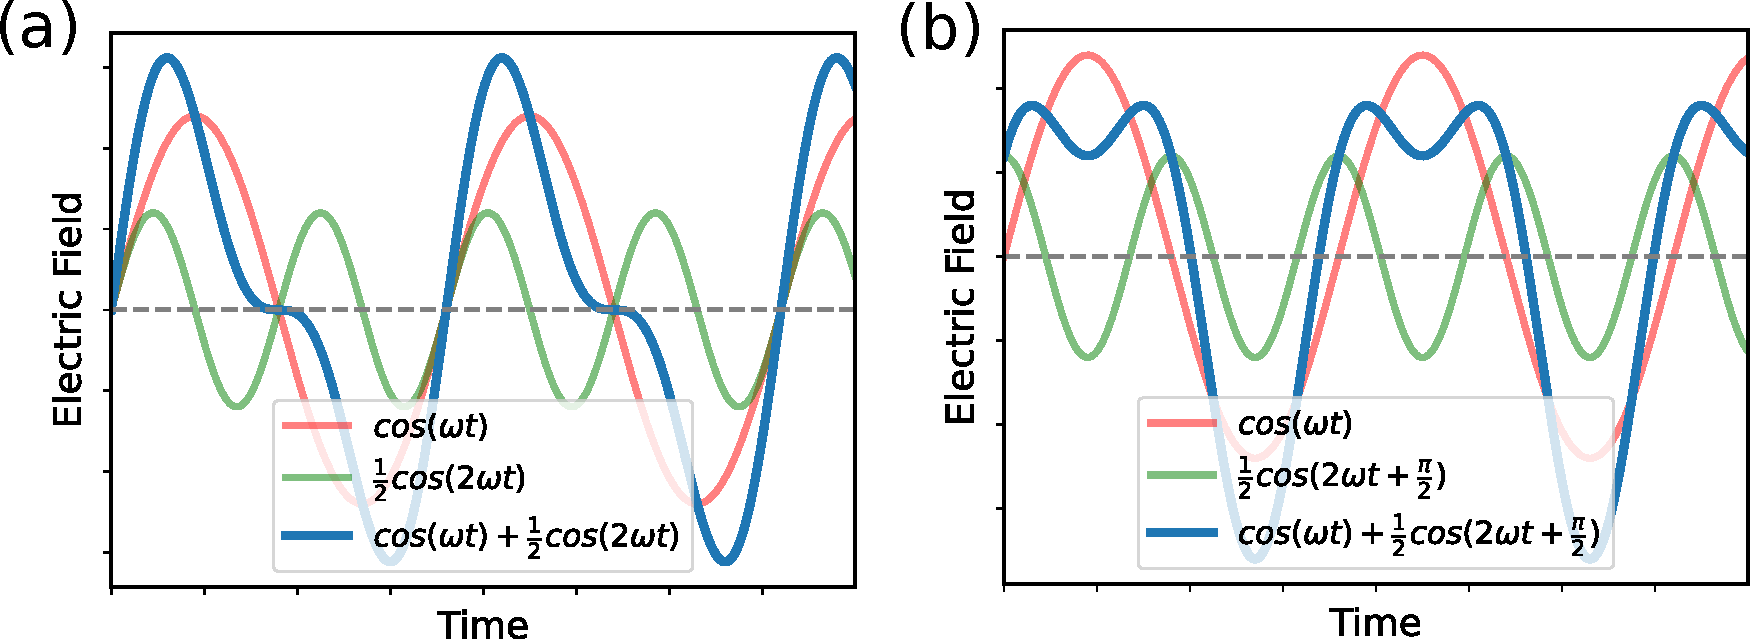
\includegraphics[width=1.0\linewidth]{pic/electric.pdf}
\caption{\label{fig:electricfield} 
The time profiles of the electric field given by Eq.~(\ref{eq:ele-pot-w-2w}) are shown for (a) $\phi=0$ and (b) $\phi=\pi/2$.}
\end{figure}


To comprehensively assess the persistent dc-current following laser irradiation, we conduct an in-depth analysis utilizing the photo-excited conduction population $n_{c\vecb{k}}$ computed from Eq.~(\ref{eq:population_tdse}). Employing a weak enough laser field in the perturbation region with a strength of $E_0=2.57$~MV/cm and fixing the relative phase at $\phi=0$, the resulting conduction population is illustrated in Fig.~\ref{fig:population}~(a). For comparative purposes, Fig.~\ref{fig:population}~(b) presents the conduction population $n_{c\vecb{k}}$ computed under the same field strength ($E_0=2.57$~MV/cm) but with a distinct relative phase ($\phi=0$). In both instances, the conduction populations exhibit notable excitations centered around the $K$- and $K'$-points. This observation implies that the photo-absorption process is primarily governed by a one-photon absorption at the photon energy of $2\hbar \omega$ and a two-photon absorption at the photon energy of $\hbar \omega$. The consistency in the excitation patterns further underscores the dominance of these absorption mechanisms in the system under the specified laser conditions.


While the population distributions in Fig.\ref{fig:population}(a) and (b) may initially appear similar, a closer examination reveals nuanced distinctions. In the scenario of the time-reversal symmetry-broken field ($\phi=0$) illustrated in Fig.\ref{fig:population}(a), the population distribution must manifest an imbalance between time-reversal Kramers pairs (e.g., $\vecb{k}$ and $-\vecb{k}$, or $K$ and $K'$). On the contrary, in the case of the time-reversal field ($\phi=\pi/2$) showcased in Fig.\ref{fig:population}(b), the population distribution $n_{c\vecb{k}}$ is anticipated to lack such a population imbalance. This discrepancy arises from the absence of a persistent current under these conditions. This nuanced analysis deepens our understanding of the intricate relationship between population distributions and the underlying time-reversal symmetry characteristics, providing crucial insights into the dynamic behavior of the system.

\begin{figure}[htbp]
\centering
 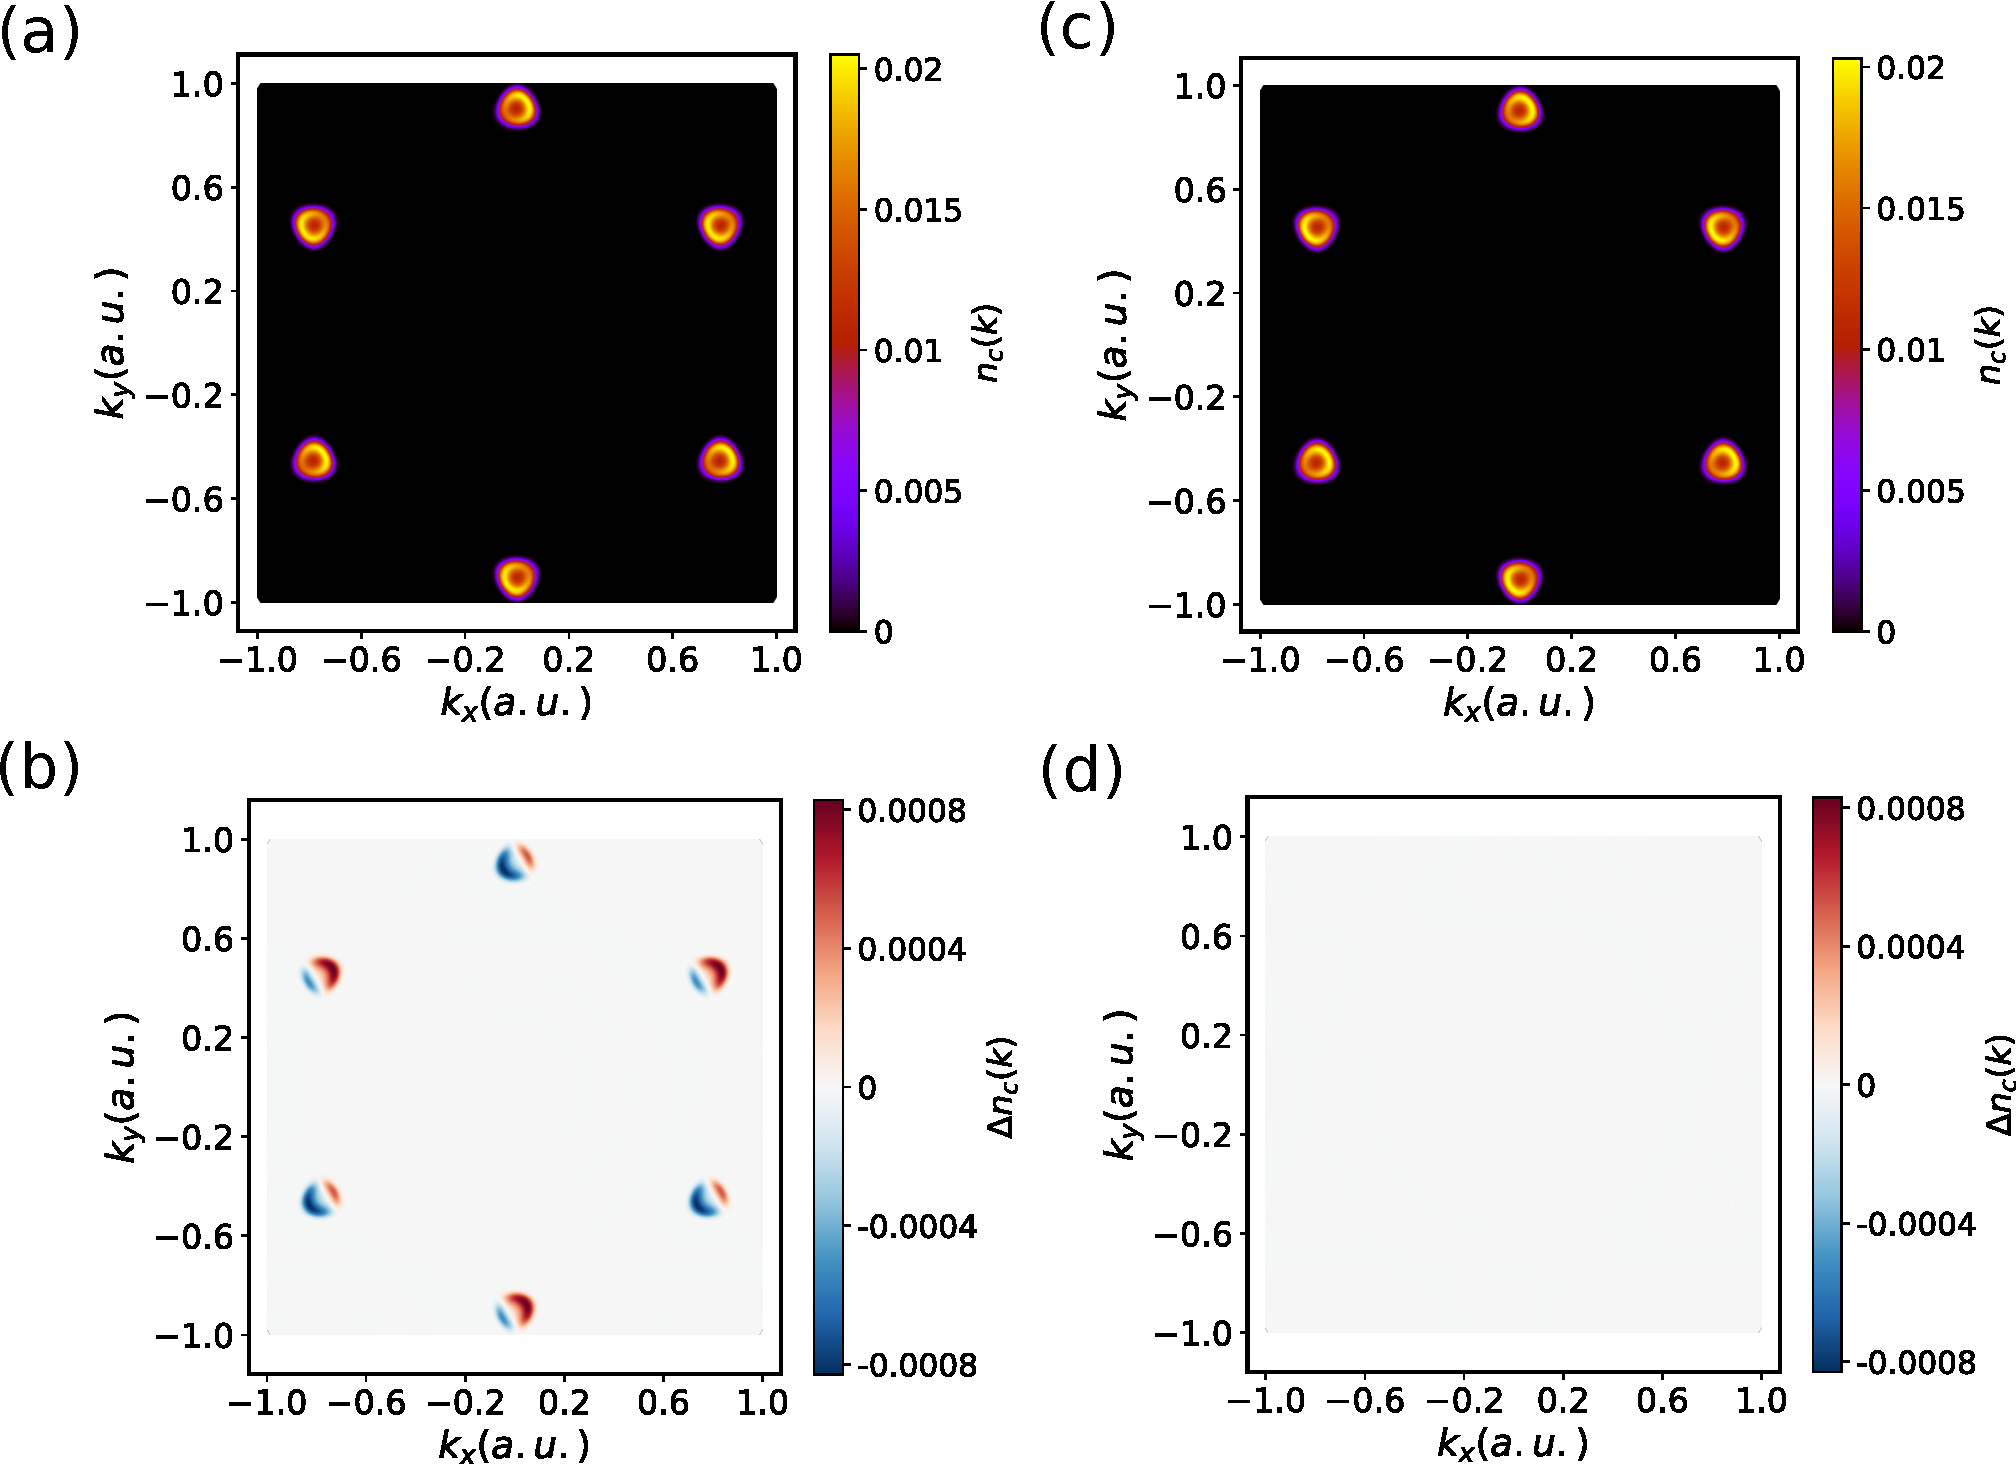
\includegraphics[width=1.0\linewidth]{pic/population.pdf}
\caption{\label{fig:population} 
(a, b) The conduction population distribution $n_c(\vecb k)$ computed with (a) $\phi=0$ and (b) $\phi=\pi/2$. (c, d) The population imbalance distribution $\Delta n_c(\vecb k)$ computed with (c) $\phi=0$ and (d) $\phi=\pi/2$.}
\end{figure}


To delineate the population imbalance across the Brillouin zone, we introduce the population imbalance distribution $\Delta n_{c\vec{k}}$, defined as the disparity in population between the time-reversal pair $k$-points, expressed as:
\begin{equation}
 \Delta n_{c\vecb{k}}=n_{c\vecb{k}}-n_{c, -\vecb{k}}  
\label{pop_imbalance }
\end{equation}
Given the constraint $0 \le n_{c\vecb{k}} \le 1$, the population imbalance distribution is bounded by $-1 \le \Delta n_{c\vecb{k}} \le 1$. In scenarios where external fields maintain time-reversal symmetry, the populations at $\vecb{k}$ and $-\vecb{k}$ are equivalent, resulting in a population imbalance distribution of zero. Conversely, in instances where time-reversal symmetry is broken, non-equivalent populations can be induced at $\vecb{k}$ and $-\vecb{k}$, giving rise to a finite population imbalance distribution $\Delta n_{c\vecb{k}}$.
Figures~\ref{fig:population}(c) and (d) depict the population imbalance distribution, $\Delta n_{c\vecb{k}}$, derived from the population distributions presented in Figs.\ref{fig:population}~(a) and (b), respectively. The figures clearly illustrate that when the external field disrupts time-reversal symmetry ($\phi=0$), a discernible finite population imbalance is induced. In contrast, when the field preserves time-reversal symmetry ($\phi=\pi/2$), the population imbalance diminishes entirely. This comprehensive analysis of the population imbalance distribution provides a detailed insight into the intricate interplay between external field characteristics and the resulting population asymmetry within the Brillouin zone.


The temporal evolution of the corresponding electric current, denoted as $\vecb{J}_{total}(t)$, can be computed using Eq.(\ref{eq:current}). This equation represents a functional dependence on the vector potential $\vecb{A}(t)$, as depicted in Fig.\ref{fig:initial_current}. The total current encompasses multiple components and noises, often overshadowing the relatively small value of the dc-component following the laser pulse. To pragmatically examine and isolate the dc-current generated by the fields, we introduce the global phase $\theta$ into the fields as described by the Eq.(\ref{eq:vec-pot-w-2w}), as done in our prior study\cite{sato2023limitations}.
\begin{equation}
\vecb{A}(t) = -\vecb{e}_p \frac{E_0}{\omega} \left [
\cos \left (\omega t + \theta \right ) + \frac{1}{4}\cos
\left (2\omega t + 2\theta + \phi \right )
\right ] \nonumber \times \cos^4 \left (\frac{\pi}{\tau}t \right )
\label{eq:vec-pot-w-2w}
\end{equation}

\begin{figure}[htbp]
\centering
 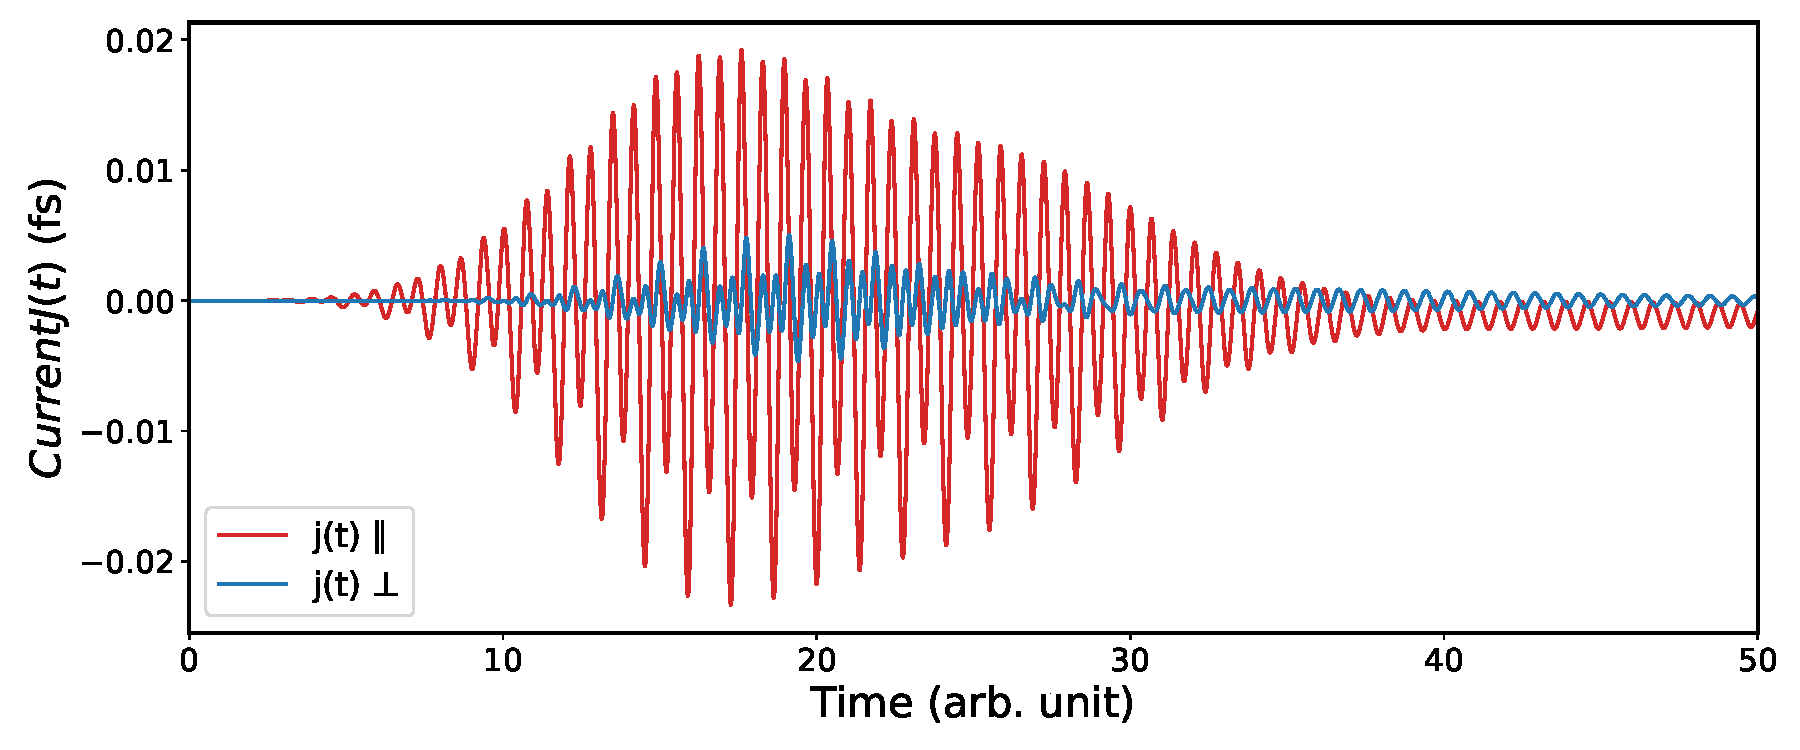
\includegraphics[width=1.0\linewidth]{pic/initial_current.pdf}
\caption{\label{fig:initial_current}} 
The time profiles of the current computed from Eq.~(\ref{eq:current}) induced by the electric field given by Eq.~(\ref{eq:ele-pot-w-2w}) as shown in Fig. ~\ref{fig:electricfield}(a) with relative phase $\phi=0$. 
\end{figure}
The current, expressed as a function of the global phase $\theta$ in accordance with the vector potential given by Eq.(\ref{eq:vec-pot-w-2w}), is explicitly denoted as $\vecb{J}(t,\theta)$. By maintaining all laser parameters constant in Eq.(\ref{eq:vec-pot-w-2w}) except for the global phase $\theta$, we can isolate the direct current (dc)-like component of the induced current through the following integral:
\begin{equation}
\vecb{J}_{\text{dc}}(t) = \frac{1}{2\pi} \int_0^{2\pi} d\theta , \vecb{J}(t,\theta).
\label{eq:dc-current}
\end{equation}
In this formulation, the integral averages out the higher-frequency components, enabling the extraction of the clean dc-like slow-frequency component of the induced current.
\begin{figure}[htbp]
\centering
 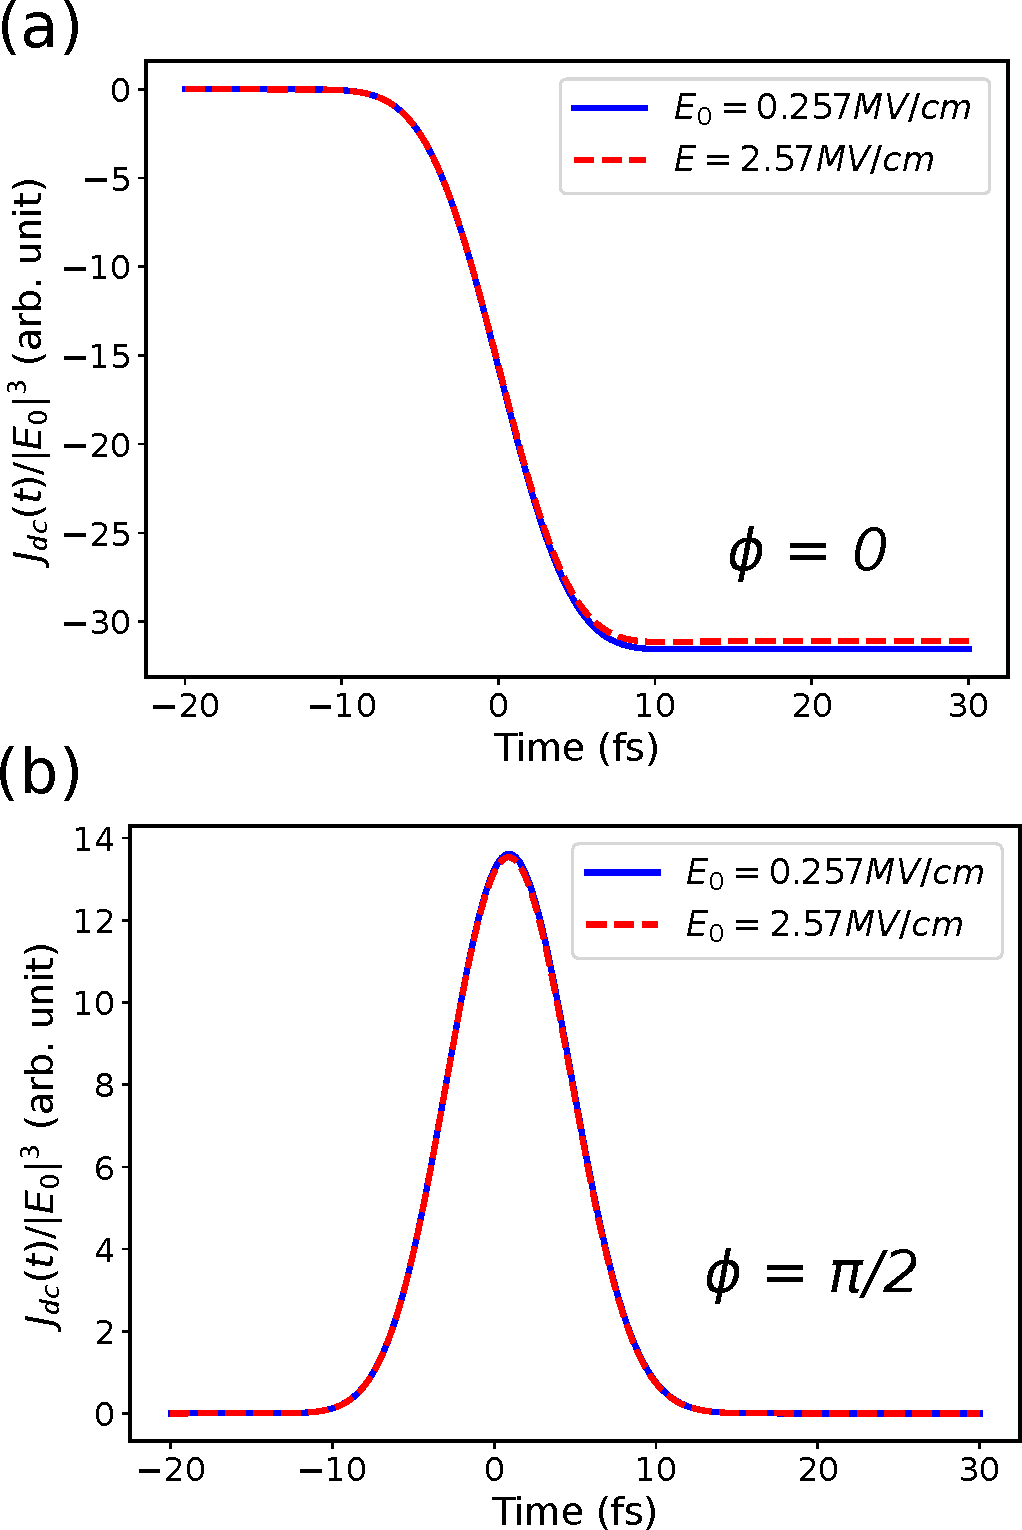
\includegraphics[width=0.8\linewidth]{pic/dc_current.pdf}:e
\caption{\label{fig:dc_current} 
The dc components of the currents $\vecb{J}_{\text{dc}}(t)$ computed from Eq.~(\ref{eq:dc-current}) are shown as a function of time. The results using the relative phase of $\phi=0$ are shown in panel (a), while those using $\phi=\pi/2$ are shown in (b) }
\end{figure}

In Figure~\ref{fig:dc_current}(a), the calculated direct current (dc) component of the scaled current, $\vecb{J}_{\text{dc}}(t)/E_0^3$, is presented for a relative phase of $\phi=0$, encompassing results for various field strengths, $E_0$. Remarkably, the residual dc-current persists beyond the conclusion of the laser fields ($t>\tau/2$). Notably, the scaled quantity, $\vecb{J}{\text{dc}}(t)/E_0^3$, maintains identical behavior across different field strengths. This consistency suggests that the dc component of the induced current can be interpreted as a third-order nonlinear optical effect. This interpretation aligns with the inherent nature of the 1+2 \gls{QuIC} process, which involves interference between one- and two-photon absorption processes, categorizing it as a third-order nonlinear optical phenomenon. The presented results shed light on the robust and field-independent nature of the observed third-order nonlinear optical effects in the system.

In Figure~\ref{fig:dc_current}(b), the dc-current component of the scaled current, $\vecb{J}_{\text{dc}}(t)/E_0^3$, is depicted with a relative phase of $\phi=\pi/2$. In stark contrast to the results with $\phi=0$ shown in Fig.\ref{fig:dc_current}(a), the currents in Fig.\ref{fig:dc_current}~(b) do not manifest a persistent dc component after the conclusion of the laser irradiation. This outcome signifies that the applied field with a relative phase of $\phi=\pi/2$ does not disrupt time-reversal symmetry, and consequently, no population imbalance is induced, resulting in the absence of a sustained current. It is noteworthy that, even in the case of $\phi=\pi/2$, the dc-component of the current is induced solely during the laser irradiation, highlighting yet another instance of a third-order nonlinear optical process. This observation provides further insight into the nuanced interplay between field characteristics and the resulting dynamical responses in the system.


By manipulating the relative phase $\phi$, one gains control over the extent of time-reversal symmetry breaking, thereby influencing the resulting population imbalance and dc- current injection~\cite{PhysRevLett.74.3596}. For subsequent analysis, we systematically explore the persistent dc current by varying the relative phase $\phi$. Figure~\ref{fig: imbalance} illustrates the dependence of the dc-current on the relative phase $\phi$ after laser irradiation, computed using a field with a strength of $E_0=2.57~$MV/cm. The amplitude of the induced dc current reaches its maximum when $\phi=0$ and $\phi=\pi$, with opposite signs for these two phases. Moreover, the induced dc current exhibits continuous variation as the phase $\phi$ is manipulated, attaining zero when $\phi=\pi/2$ and $\phi=3\pi/2$, corresponding to the points where the applied fields restore time-reversal symmetry. This straightforward phase dependence aligns with findings from prior works\cite{PhysRevLett.74.3596,PhysRevLett.78.306}, providing further validation of the controllable nature of the induced dc current through manipulation of the relative phase.

\begin{figure}[htbp]
\centering
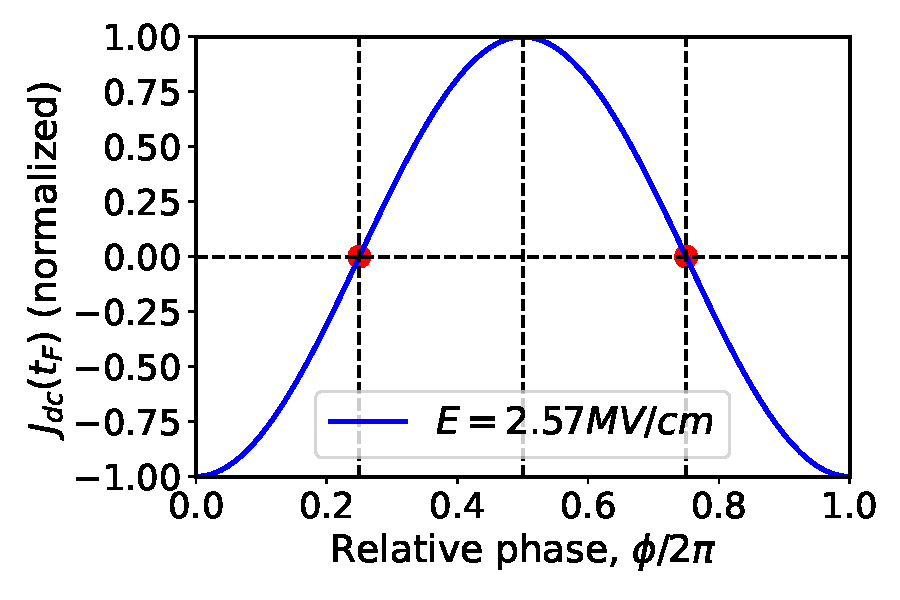
\includegraphics[width=0.8\linewidth]{pic/relativephase.pdf}
\caption{\label{fig: imbalance} 
The persistent current $J_{\text{dc}}(t_f)$ as a function of the relative phase, $\phi$. The results are computed by setting $E_0$ to $2.57$~MV/cm and $\hbar \omega$ to 3~eV.}
\end{figure}


\gls{QuIC} processes often exhibit resonance conditions at specific photon energies. By systematically investigating the photon-energy dependence, we can identify resonant regions where the interference effects are significantly enhanced.  Investigating these dependencies aids in identifying the primary mechanisms at play. To scrutinize this phenomenon within our theoretical framework, we systematically evaluate the direct current (dc) after laser irradiation by varying the fundamental frequency $\omega$ in Eq.(\ref{eq:vec-pot-w-2w}). Figure\ref{fig:fig4}~(a) illustrates the resulting dc current following laser irradiation with a field strength of $E_0=1.03$~MV/m. 

In line with the anticipated behavior of the $1+2$~\gls{QuIC} process, the residual dc-current diminishes when the fundamental photon energy falls below half of the band gap, i.e., $\hbar \omega \le E_g/2 = 2.95$~eV,  since the fundamental photon energy $\hbar \omega$ must adhere to the condition $\hbar \omega \ge E_g/2$, where $E_g$ signifies the band gap. 
In instances where the fundamental photon energy $\hbar \omega$ falls below the gap, both the $1+2$~QuIC process and the resultant direct current (dc) vanish. This exploration not only elucidates the pivotal role of photon energy in the manifestation of the $1+2$~\gls{QuIC} process but also underscores the significance of satisfying specific conditions for its occurrence and subsequent dc-current induction.
This behavior aligns with the expected characteristics of the $1+2$~\gls{QuIC} process and provides valuable insights into the influence of the fundamental frequency on the induced dc-current in our theoretical framework.
\begin{figure}[htb]
\centering
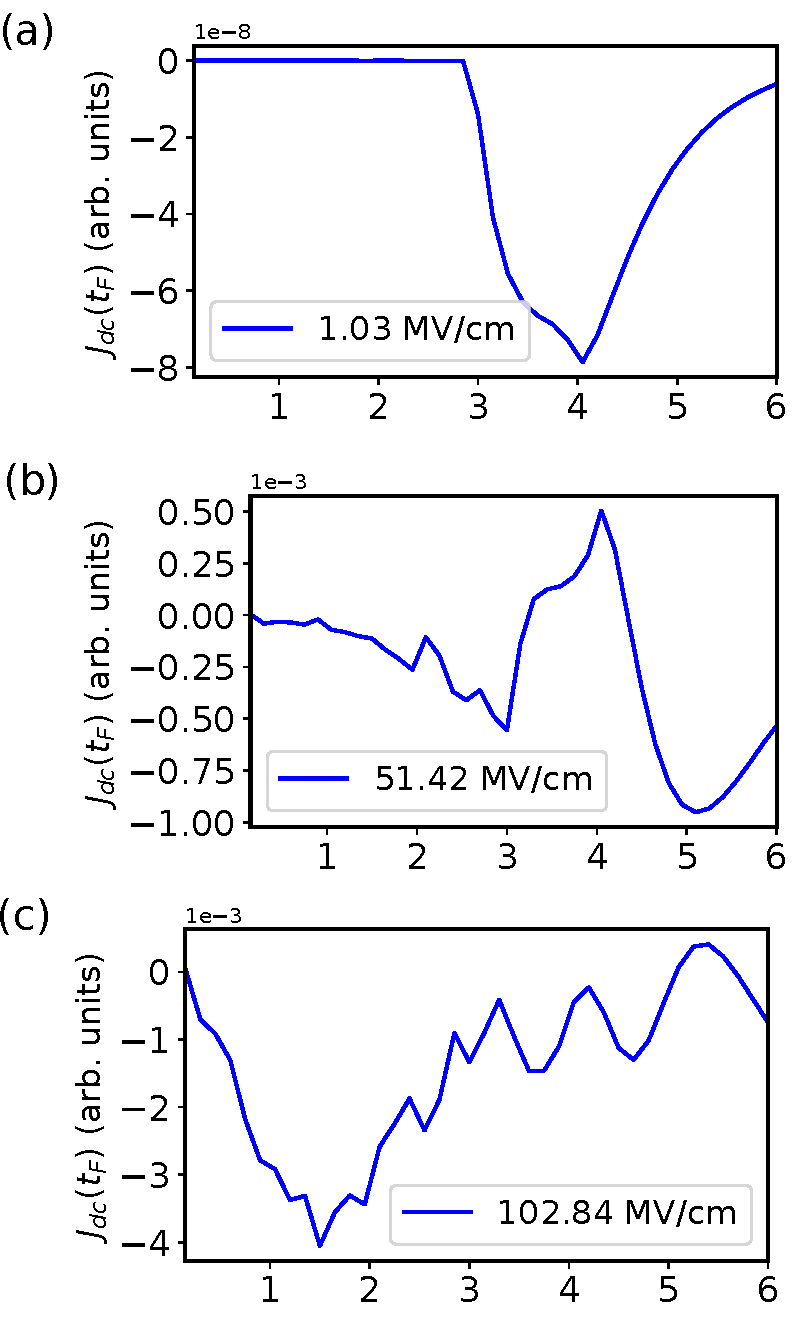
\includegraphics[width=0.8\linewidth]{pic/frequency.pdf}
\caption{\label{fig:fig4} 
The current after the laser irradiation is shown as a function of the fundamental photon energy $\hbar \omega$. The results computed different field strengths: (a) $E_0=1.03$~MV/cm, (b) $51.43$~MV/cm, and (c) $E_0=102.84$~MV/cm.}
\end{figure}

 The investigation aids in comprehending the intricate relationship between photon energy, field strength, and the ensuing nonlinear processes. It is imperative to investigate the photon energy dependence of the direct current (dc) after laser irradiation while systematically varying the field strength, $E_0$, to unravel the intricacies of this highly nonlinear optical phenomenon. 
 Figures~\ref{fig:fig4}~(b) and (c) meticulously depict the photon-energy dependence of the persistent current following laser irradiation, calculated for two distinct field strengths: (b) $E_0=51.42$~MV/cm and (c) $E_0=102.84$~MV/cm. In stark contrast to the weak field regime typified by the $1+2$~\gls{QuIC}, the direct current (dc) can be induced even under deeply off-resonant conditions, where the photon energy is smaller than half of the band gap ($\hbar \omega \le E_g/2$), as evident in Figure\ref{fig:fig4}(b). This compelling observation suggests that potent laser fields introduce additional pathways for electron excitation that extend beyond the realm of two-photon absorption. These additional processes, involving multiple photons, contribute to the creation of a population imbalance and a residual dc current, even in the deeply off-resonant regime. The nuanced interplay between laser field strength and photon energy unveiled in these results provides invaluable insights into the complex dynamics governing persistent currents in strong-field regimes.

 Illustrated in Figure~\ref{fig:fig4}~(c), a noteworthy observation emerges the magnitude of the direct current (dc) after laser irradiation in the deeply off-resonant regime ($\hbar \omega \le E_g/2$) surpasses that in the $1+2$~\gls{QuIC} regime ($\hbar \omega \ge E_g/2$) as the applied field strength reaches exceptionally large values. This intriguing behavior finds its explanation in the ponderomotive energy, denoted as:
 \begin{align}
 U_p=\frac{e^2E^2_0}{4m\pi \omega_0^2}    
 \end{align}
 The associated light-induced intraband transitions, both of which are more substantial for lower frequency driving\cite{PhysRevB.98.035202}. Consequently, the ensuing nonlinear effects and the injection of dc current become more pronounced in the deeply off-resonant regime compared to the resonant condition. 
Our initial investigation focused on analyzing the electric current induced by these two-color laser fields within the weak field regime. We confirmed that the dc-component of the induced current persists even after laser irradiation when the fundamental photon energy $\hbar \omega$ exceeds the optical gap, $E_g/2$. This ballistic current phenomenon originates from a population imbalance in the Brillouin zone, arising from quantum interference between two distinct excitation paths: one involving one-photon absorption at the photon energy of $2\hbar \omega$, and the other involving a two-photon absorption path at the photon energy of $\hbar \omega$~\cite{PhysRevLett.74.3596,PhysRevLett.76.1703,PhysRevLett.78.306}.


 This discovery sets the stage for a more in-depth exploration in the subsequent section, where we will delve into the intricacies of efficiently inducing DC current through highly nonlinear optical processes in the deeply off-resonant regime.


%%%%%%%%%%%%%%%%%%%%%%%%%%%%%%%%%%%%%%%%%%%%%%%%%%%%%%%%%%%%%%%%%%%%%%%%%%%%%%%%%%%
\section{Deeply off-resonant highly-nonlinear regime \label{sec:nonperturbative}}
%%%%%%%%%%%%%%%%%%%%%%%%%%%%%%%%%%%%%%%%%%%%%%%%%%%%%%%%%%%%%%%%%%%%%%%%%%%%%%%%%%%

Despite the significant interest in the nonlinear photovoltaic effect, there has been limited exploration of efficient current injection in the deeply off-resonant regime with multi-cycle light pulses, particularly using linearly polarized light. Subsequently, the scope of \gls{QuIC} can be broadened to involve general integer combinations, denoted as $M+N$~\gls{QuIC}~\cite{PhysRevB.100.075202,PhysRevLett.123.067402}. In this extended scheme, two-color laser fields operating at frequencies $\omega$ and $\omega'$ induce $M$- and $N$-photon absorption processes, respectively.
To investigate the mechanism of dc-current injection in the deeply off-resonant regime, as demonstrated in the previous section, we fix the fundamental photon energy $\hbar \omega$ in Eq.~(\ref{eq:vec-pot-w-2w}) at $1$~eV. Notably, this value is much smaller than half of the band gap, $E_g/2=2.95$~eV, for this section.

\begin{figure}[htb]
\centering
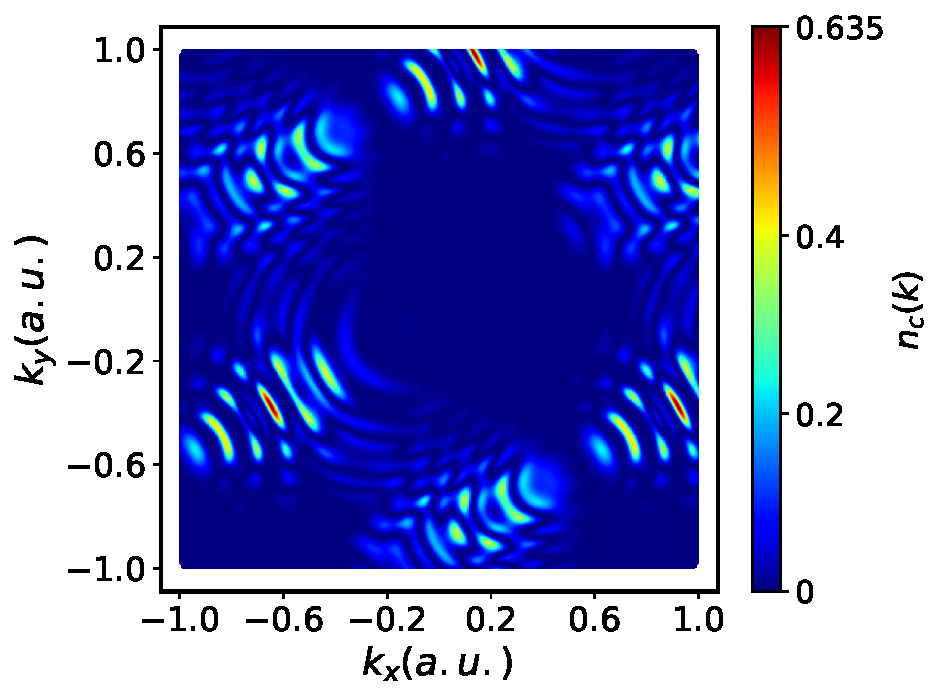
\includegraphics[width=0.8\linewidth]{pic/nex_pop_E0_1e10.pdf}
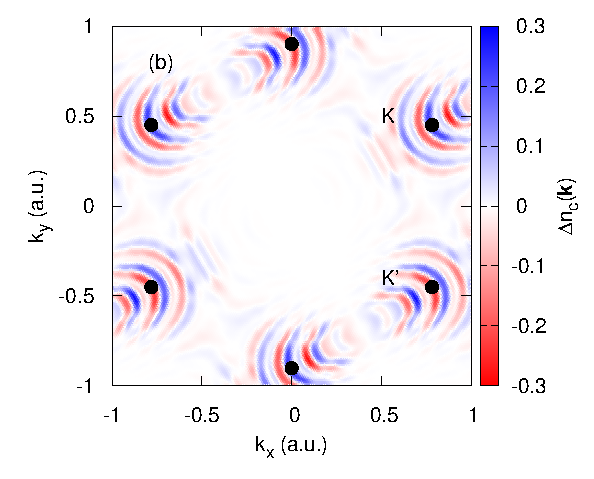
\includegraphics[width=0.8\linewidth]{pic/dnex_pop_E0_1e10.pdf}
\caption{\label{fig:nex_pop_E0_1e10} 
(a) The conduction population distribution $n_{c}(\vecb k)$ after the irradiation of the laser field, and (b) the population imbalance distribution $\Delta n_c (\vecb k)$ are shown. The results are computed by setting $E_0$ to $10^{10}$~V/m.
}
\end{figure}

Similarly, we start with evaluating the population imbalance induced by a strong field in the
deeply off-resonant regime, we calculate the population distribution $n_{c\vec{k}}$ after
irradiating the laser field with a strength of $100$~MV/cm. A distinct pattern emerges in the excited carrier population distribution around the $K$ and $K'$ points. This pattern can be understood through the multi-photon absorption resonances of the light-induced Floquet states\cite{galler2023mapping}. In Fig.\ref{fig:nex_pop_E0_1e10}(a), we present the computed population distribution in the conduction band. As anticipated from the preceding discussion, the photo-carrier distribution reveals a significant population imbalance between $\vecb{k}$ and $-\vecb{k}$ points. To enhance clarity in visualizing the population imbalance, we compute the population imbalance distribution $\Delta n_{c\vecb{k}}=n_{c\vecb{k}}-n_{c, -\vecb{k}}$. Figure~\ref{fig:nex_pop_E0_1e10}(b) displays the resulting population imbalance distribution $\Delta n_{c\vecb{k}}$. Since $\Delta n_{c\vecb{k}}$ is constrained by $-1\le \Delta n_{c\vecb{k}} \le 1$, the population imbalance between $\vecb{k}$ and $-\vecb{k}$ is maximized when $|\Delta n_{c\vecb{k}}|=1$. As observed in Fig.\ref{fig:nex_pop_E0_1e10}~(b), the population imbalance distribution takes significantly large values, comparable to the maximum values ($\pm 1$), across a wide range of the Brillouin zone.
\begin{figure}[htbp]
\centering
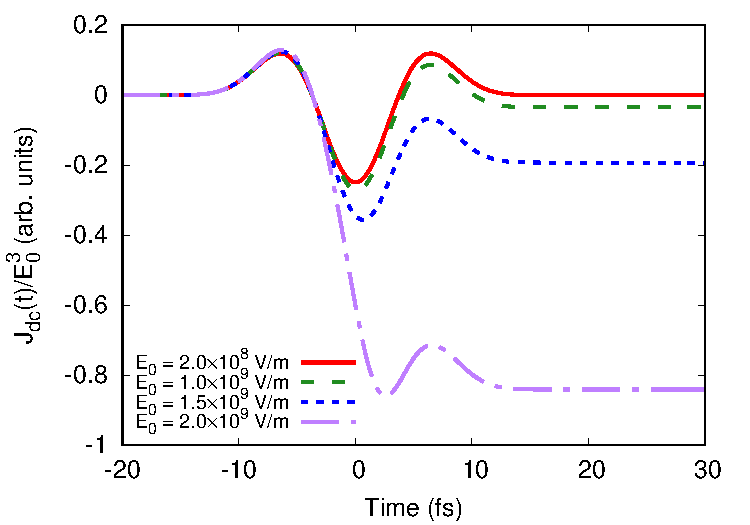
\includegraphics[width=0.8\linewidth]{pic/current_off_resonant.pdf}
\caption{\label{fig:current_off_resonant} 
The dc components of the currents, $\vecb J_{dc}(t)$, are shown as a function of time. The results are computed with the deeply off-resonant condition, $\hbar\omega = 1.0$~eV.}
\end{figure}

We calculate the population imbalance ratio $r_{im}$ defined as the maximum absolute value of the
population imbalance distribution $\Delta n_{c\vecb{k}}$ across the Brillouin zone for further
qualification. Mathematically, it is expressed as:
\begin{equation}
r_{im} = \frac{\int_{BZ}d\vecb k \left |\Delta n_{c\vecb{k}} \right |}{\int_{BZ}d\vecb k \left (n_{c\vecb{k}} + n_{c,-\vecb{k}}\right )}
= \frac{\int_{BZ}d\vecb k \left |\Delta n_{c\vecb{k}} \right |}{2\int_{BZ}d\vecb k n_{c\vecb{k}}}.
\end{equation}
The computed imbalance ratio, $r_{im}$, from Figs.\ref{fig:nex_pop_E0_1e10}(a) and (b) is about
0.307. Hence, more than 30\% of the excited electrons contribute to the population imbalance.
This implies the potential for realizing a significant population imbalance through the use of linearly polarized light alone.

In an earlier study~\cite{Jimenez-Galan2020}, significant control over valley population was proposed using bi-circular fields with counter-rotating $\omega$ and $2\omega$ two-color laser fields. In contrast, in this work, we demonstrate that significant valley population can be induced without relying on circular or elliptically polarized light; rather, bi-color linearly polarized light alone can break the time-reversal symmetry and cause such population control.


We commence our analysis of population imbalance by examining the light-induced current in the time domain within the deeply off-resonant regime. In Figure~\ref{fig:current_off_resonant}, we present the dc component of the current, $\vecb{J}_{\text{dc}}(t)/E_0^3$, computed with varying field strengths, $E_0$. For this analysis, the relative phase $\phi$ is set to 0. Evidently, a third-order nonlinear response dominates the induced current in the case of weak field strength. Given that the photon energy of the second harmonic is smaller than the band-gap ($2\hbar \omega < E_g$) and the \gls{QuIC} process is forbidden, the third-order current returns to zero after the laser irradiation.

However, as the field strength becomes sufficiently strong, the dc-component remains finite even after laser irradiation, as depicted in Fig.~\ref{fig:current_off_resonant}. This observation suggests that a higher-order nonlinear process contributes to the ballistic dc-current injection beyond the third-order nonlinear effect.

\begin{figure}[htbp]
\centering
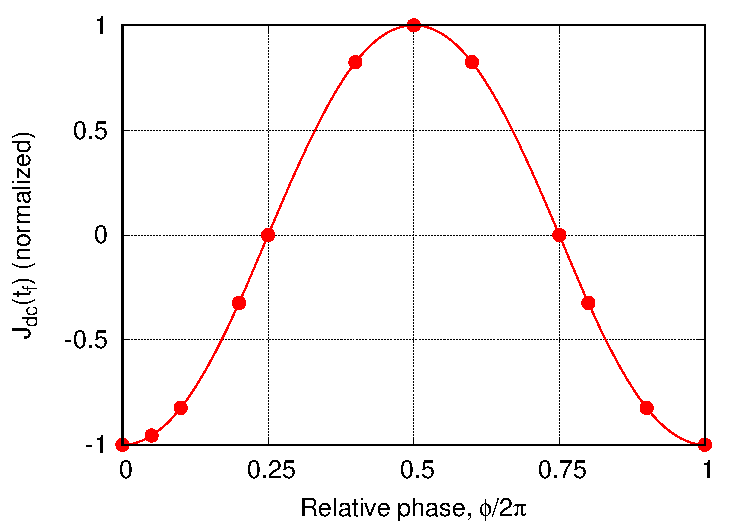
\includegraphics[width=0.8\linewidth]{pic/jdc_vs_phi_off_resonance.pdf}
\caption{\label{fig:jdc_vs_phi_off_resonance} 
The persistent current, $J_{dc}(t_f)$, is shown as a function of the relative phase $\phi$. The results are computed with the deeply off-resonant condition, $\hbar\omega = 1.0$~eV.
}
\end{figure}

Next, we explore the dependence of the ballistic current induced by deeply off-resonant light on
the relative phase, $\phi$. Figure~\ref{fig:jdc_vs_phi_off_resonance} illustrates the computed
current as a function of the relative phase, $\phi$, with calculations conducted at a field
strength of $E_0=2 \times 10$MV/cm. In accordance with the QuIC case shown in Fig.\ref{fig:
imbalance}, the persistent current is maximized when the relative phase is $\phi=0$ or $\phi=\pi$,
and it vanishes when the applied field exhibits time-reversal symmetry ($\phi=\pi/2$ or
$\phi=3\pi/2$). Therefore, even in the deeply off-resonant regime, the direction and magnitude of
the persistent current can be controlled by manipulating the relative phase $\phi$ between the
two-color fields at frequencies $\omega$ and $2\omega$.\\

\begin{figure}[htbp]
\centering
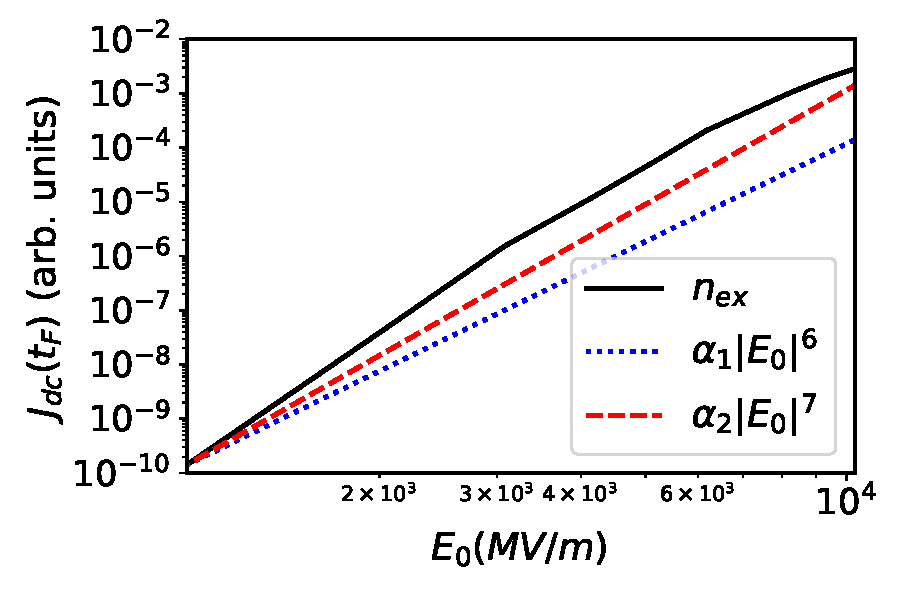
\includegraphics[width=0.80\linewidth]{pic/dc_current_vs_E0.pdf}
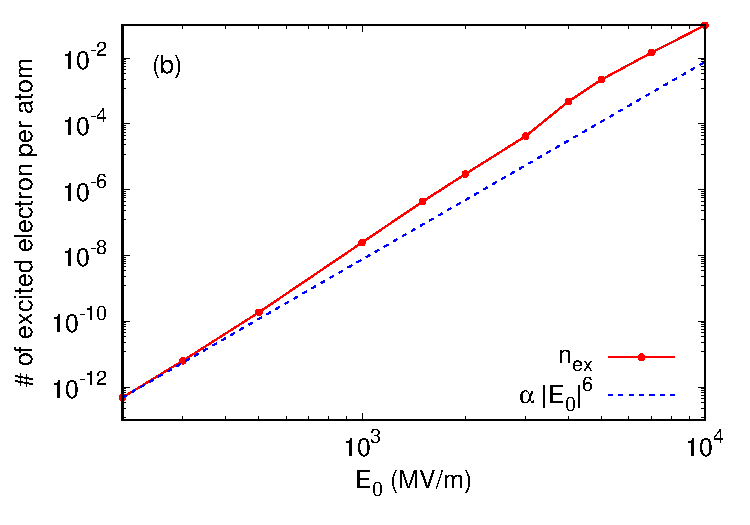
\includegraphics[width=0.80\linewidth]{pic/nex_vs_E0.pdf}
\caption{\label{fig:dc_current_vs_E0} 
(a) The persistent current, $|J_{dc}(t_f)|$, is shown as a function of the field strength, $E_0$. (b) The number of conduction population after the laser irradiation is shown as a function of the field strength $E_0$.
}
\end{figure}
To gain a more detailed understanding of the intricate mechanism behind dc current injection in the deeply off-resonant regime, we delve into an analysis of how the injected current scales with the applied field strength $E_0$. As depicted in Figure~\ref{fig:dc_current_vs_E0}, the current amplitude after laser irradiation is plotted against the varying field strength. Notably, a reference line representing $|E_0|^7$ is included for comparison.

The compelling observation from the figure is that the induced current exhibits a clear proportionality to $|E_0|^7$ in the weak field regime. This insightful finding suggests that the seventh-order nonlinear process takes precedence in governing the dynamics of dc current injection under these conditions. This nuanced understanding provides a comprehensive insight into the intricate nonlinear optical processes that contribute to the observed dc current phenomena in the deeply off-resonant regime.

The observed scaling law of the induced dc current with the applied field strength might initially
seem inconsistent with the expected behavior of a straightforward $M+N$ \gls{QuIC} process. In the
conventional $M+N$ \gls{QuIC} scenario, the $M$-photon absorption process is initiated by light with frequency $\omega$, and the $N$-photon absorption process is triggered by light with frequency $2\omega$, resulting in an overall $(M+N)$-th order nonlinear process. For instance, if we consider a six-photon process for multi-photon absorption with light of frequency $\omega$ and a three-photon process for light of frequency $2\omega$, the anticipated simple $M+N$ QuIC process corresponds to the ninth-order nonlinear process ($M+N=6+3=9$).

However, our experimental observations reveal a scaling that indicates seventh-order nonlinearity instead. This apparent discrepancy in the observed and expected nonlinearities of the injected dc current can be rationalized by the presence of an additional excitation channel involving a four-photon absorption process. In this scenario, two photons at frequency $\omega$ and the other two photons at frequency $2\omega$ combine to excite electrons. This additional four-photon excitation channel interferes with the three-photon absorption process at the photon energy of $2\hbar \omega$, resulting in seventh-order ($7=3+4$) nonlinear current injection.

To delve deeper into the nonlinearity of the light-induced electron dynamics, we performed computations to determine the number of photo-excited carriers after laser irradiation using the expression:
\begin{align}
N_{ex} = \frac{2}{A_{\mathrm{BZ}}}\int_{\mathrm{BZ}} d\vecb{k} n_{c,\vecb{k}}, 
\end{align}
where $A_{\mathrm{BZ}}=\int_{\mathrm{BZ}} d\vecb{k}$ represents the area of the Brillouin zone.

Figure~\ref{fig:dc_current_vs_E0}~(b) presents the number of excited electrons as a function of the field strength, $E_0$, alongside a reference line proportional to $|E_0|^6$. In the weak field regime, the number of excited electrons exhibits proportionality to $|E_0|^6$, highlighting the dominance of the three-photon absorption process in the excitation mechanism. However, as the field strength increases, the deviation from the three-photon absorption line suggests the initiation of a nonperturbative mechanism in the excitation process.

In contrast to the $|E_0|^6$-dependence of the number of photo-excited carriers in the weak field regime, the injected current and the corresponding population imbalance follow a $|E_0|^7$ scaling, as depicted in Figure~\ref{fig:dc_current_vs_E0}~(a). The difference in nonlinearities between the absolute photo-carrier population and the population imbalance implies that the population imbalance is negligible concerning the absolute photo-carrier population in the weak field regime. However, in a strong field regime, the relative significance of the population imbalance becomes substantial as it grows more rapidly than the absolute photo-carrier population. Therefore, the distinction in nonlinearities between the total photocarrier population and the population imbalance indicates the potential for large-amplitude valley carrier population control.

Expanding our analysis to the deeply off-resonant regime, where $\hbar \omega \ll E_g/2$, we observed an absence of population imbalance under weak applied field strength. However, as the field strength increased, a population imbalance in the Brillouin zone is formed, leading to the injection of the persistent dc-current after the laser irradiation. Scaling analysis of the ballistic current injection with respect to the applied field strength $E_0$ revealed that the population imbalance and the ballistic current result from an interference between three-photon absorption process with three photons of energy $2\hbar \omega$ and a four-photon absorption process with two photons of energy $2\hbar \omega$ and two photons of energy $\hbar \omega$. Consequently, we demonstrated that a multi-photon absorption process, incorporating photons with different energies, plays a pivotal role in addition to the multi-photon absorption process involving single-color photons.


In previous works~\cite{Jimenez-Galan2020,Mrudul:21,PhysRevLett.127.126601}, the formation of substantial population imbalance and valley-population control has been discussed in monolayer systems such as monolayer $h$-BN and graphene, using bi-circular laser fields with frequencies $\omega$ and $2\omega$. Recently, valley-population control with bi-circular fields has been extended to multi-layer and bulk systems~\cite{tyulnev2023valleytronics} without relying on intrinsic inversion symmetry breaking and the Berry curvature at the valleys. In contrast to these works, our study demonstrates the induction of a large population imbalance and ballistic current injection without relying on the ellipticity of light. Instead, we rely on time-reversal symmetry breaking achieved through relative phase control between two-color linearly-polarized fields at frequencies $\omega$ and $2\omega$. Furthermore, similar to Ref.~\cite{tyulnev2023valleytronics}, the injection mechanism with bi-color linearly polarized light does not rely on intrinsic inversion symmetry breaking, indicating an efficient dc current injection and population control with the scheme using linearly-polarized light. The potential of population control and the photovoltaic effect with linearly polarized light, in addition to circularly/elliptically polarized light, unveils novel avenues for realizing ultrafast opto-electronics, marked by precise control of current and population dynamics on the femtosecond time scale.


%%----------------------------------------------------------------------------------------
% CHAPTER THREE
%----------------------------------------------------------------------------------------
\chapter{THZ-INDUCED HHG AND NONLINEWAR CHARGE TRANSPORT \label{ch:ch4}}

Researchers have probed HHG in graphene particularly within the  THz regime \cite{hafez2018extremely,kovalev2021electrical}. THz-induced transparency of graphene, an interesting nonlinear optical effect, has been explored \cite{Hwang2013,Paul_2013,doi:10.1063/1.4902999}, often analyzed through a thermodynamic model emphasizing the reduction of electric conductivity \cite{mics2015thermodynamic,kovalev2021electrical}.
Despite these advancements, a comprehensive understanding of the microscopic mechanisms controlling these nonlinear effects remains tricky. The existing studies predominantly rely on thermodynamic models, lacking a thorough exploration of nonequilibrium quantum dynamics under dissipation. This research gap highlights the need for a deeper exploration of the underlying microscopic processes to unravel the intricacies of HHG and related nonlinear optical effects in graphene.

In this chapter, we investigate into the complex details of  THz-induced \gls{HHG} and nonlinear electric transport in graphene. Our approach involves utilizing the quantum master equation with the relaxation time approximation to provide a comprehensive understanding of the underlying phenomena in Chapter.~(\ref{sec:master}). To gain microscopic insights, we thoroughly compare the outcomes of fully dynamic calculations with those obtained through a quasi-static approximation,  the electronic system is treated as a nonequilibrium steady state.

The key revelation from our investigation is that the THz-induced electron dynamics in graphene can be accurately represented by the nonequilibrium steady-state approach at each moment in time. Through a thorough population distribution analysis, we clarify that THz-induced HHG in graphene arises from the reduction of effective conductivity, attributed to a significant displacement of electrons in the Brillouin zone.

To deepen our understanding, we draw comparisons between the nonequilibrium picture presented here and a thermodynamic perspective. This comparative analysis allows us to unravel the central role of the nonequilibrium nature of electron dynamics in driving the extremely nonlinear optical and transport phenomena observed in graphene. Our study contributes valuable insights into the complex interplay between THz fields, electron dynamics, and nonlinear behavior in graphene systems.

The comprehensive dynamical analysis derived from the quantum master equation provides a natural framework for understanding the complex nonequilibrium features inherent in field-induced phenomena. Specifically, it allows for the exploration of phenomena characterized by symmetry breaking and delayed responses, uncovering the dynamics of the system under the influence of external fields. Ongoing theoretical investigations aim to investigate deeper into these aspects, explaining the nonequilibrium behavior induced by light-matter interactions.
%%%%%%%%%%%%%%%%%%%%%%%%%%%%%%%%%%%%%%%%%%%%%%%%%%%%%%%%%%%%%%%%%%%%%%%%%%%%%%%%%%%%%%%%%%%%%%%%%%%%%%%%%%%%%%%%%%%%%%%%%%%%%%%%
\section{Fully Dynamical Simulations for THz Field}
%%%%%%%%%%%%%%%%%%%%%%%%%%%%%%%%%%%%%%%%%%%%%%%%%%%%%%%%%%%%%%%%%%%%%%%%%%%%%%%%%%%%%%%%%%%%%%%%%%%%%%%%%%%%%%%%%%%%%%%%%%%%%%%%

In this section, we first give a brief introduction of recent Experiments and Thermodynamic model on
graphene. Next we investigate into the microscopic intricacies controlling the THz-induced \gls{HHG} in graphene, the electronic structure is discriped by the tight-binding
model in Chapter\ref{ch:ch2}.
We initiate our investigation by conducting a detailed electron dynamics simulation using \gls{TDSE},Eq.~(\ref{eqn:masterequation}). The focus of this simulation is to analyze the \gls{HHG} in graphene under the influence of a linearly polarized laser pulse. To promote this analysis, we adopt a specific form for the applied vector potential, described by the equation:

\begin{align}
	\mathbf A(t) = -\frac{E_0}{\omega_0}\mathbf{e_x} \sin(\omega_0 t)\cos^4 \left (\frac{\pi}{T_\mathrm{full}} t \right),
	\label{eqn:laser_pulse}
\end{align}

where the simulation is conducted in the domain $-T_\mathrm{full}/2 < t < T_\mathrm{full}/2$ and is zero outside this period. Aligning with a previous experimental setup \cite{hafez2018extremely}, we set specific parameters for the pulse: the peak field strength $E_0$ is chosen as $8.5$~MV/m, the mean photon energy $\hbar \omega_0$ is set to $1.2407$~meV, and the pulse duration $T_{\mathrm{full}}$ is established as $40$~ps. Notably, the direction of the electric field $\mathbf e_x$ is defined along the $\Gamma$--$M$ direction.

This detailed setup enables a thorough exploration of the electron dynamics under the influence of the specified laser pulse parameters, laying the groundwork for a comprehensive analysis of high-order harmonic generation in graphene.

Following the electron dynamics simulation governed by the field in Eq.~(\ref{eqn:laser_pulse}), solve the quantum master euation in Eq.~(\ref{eqn:masterequation}) with the vector potential given above, we obtain the time-dependent density matrix. Then we proceed to compute the induced electric current, denoted as $\mathbf J(t)$ given by Eq.~(\ref{eqn:totalcurrent}). To unveil the frequency content embedded within the current dynamics, we employ a Fourier transform applied to the current, yielding the high-order harmonics spectrum described by the expression:

\begin{align}
	I_{\mathrm{HHG}}(\omega)\sim \omega^2 \left | \int^{\infty}_{-\infty} dt , J(t) , e^{i\omega t} \right |^2.
	\label{eqn:spectrum}
\end{align}

Here, $I_{\mathrm{HHG}}(\omega)$ encapsulates the contribution of high-order harmonics, and the spectrum is determined by the square of the magnitude of the Fourier transform of the induced current. This approach enables us to discern and analyze the harmonic content within the electric current, providing valuable insights into the high-order harmonic generation phenomenon induced by the specified laser pulse.

\begin{figure}[htbp]
	\centering
	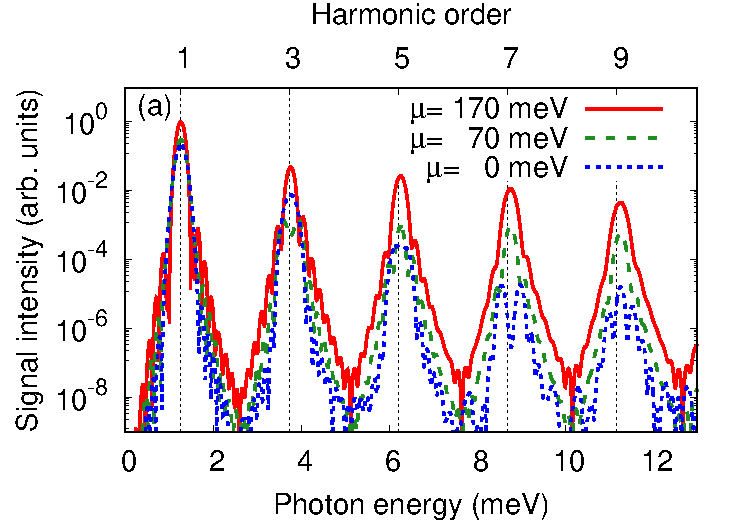
\includegraphics[width=0.8\linewidth]{pic/hhg_mu.pdf}
	\caption{\label{fig:hhg_mu}
		Computed harmonic spectra $I_{\mathrm{HHG}}(\omega)$ with Eq.~(\ref{eqn:spectrum}) for different
		chemical potentials, $\mu = 0$, $70$ and $170$~meV. Figure is reproduced with permission from ref.~(\cite{PhysRevB.106.024313}). Copyright 2022, Phys. Rev. B.}
\end{figure}

In Figure~\ref{fig:hhg_mu}, we present the computed HHG spectra, denoted as $I_{\mathrm{HHG}}(\omega)$, corresponding to different chemical potentials $\mu$. Each chemical potential yields distinct harmonic peaks, and a noticeable trend emerges: the intensities of the induced harmonics systematically increase with the rise in the chemical potential. This observation combines with findings from a recent experiment \cite{kovalev2021electrical}, where an analogous increase in induced harmonic intensity was noted with an elevation in gate voltage.

The observed trends in harmonic spectra intensities presented here depending on the chemical potential increasing reproduce the results from former research, such as \cite{mics2015thermodynamic}, where THz-induced high-order harmonic generation in graphene was clarifyd through a thermodynamic framework. In contrast, our current study aims to advance the understanding of these THz-induced nonlinear phenomena by considering a comprehensive microscopic perspective. Specifically, we investigate into the nonequilibrium nature of electron dynamics to process our description of light-matter interactions and provide a more  interpretation of the observed trends in high-order harmonic spectra with varying chemical potentials.

Following the electron dynamics calculations under THz fields, our findings reveal that the induced harmonics experience enhancement with an increase in chemical potential. This theoretical insight combines with recent experimental observations, where high-order harmonic generation is similarly enhanced through the application of a gate bias voltage \cite{kovalev2021electrical}.
%%%%%%%%%%%%%%%%%%%%%%%%%%%%%%%%%%%%%%%%%%%%%%%%%%%%%%%%%%%%%%%%%%%%%%%%%%%%%%%%%%%%%%%%%%%%%%%%%%%%%%%%%%%%%%%%%%%%%%%%%%%%%%%%%%
\section{Quasi-static Approximation}
%%%%%%%%%%%%%%%%%%%%%%%%%%%%%%%%%%%%%%%%%%%%%%%%%%%%%%%%%%%%%%%%%%%%%%%%%%%%%%%%%%%%%%%%%%%%%%%%%%%%%%%%%%%%%%%%%%%%%%%%%%%%%%%%%%
Subsequently, we introduce a quasi-static approximation to investigate the THz-induced electron dynamics, halping a reexamination of the nonlinear electric transport and the field-induced transparency phenomena inherent to graphene \cite{sato2021nonlinear}.
In our analysis, we make the assumption that the variation of the THz field is sufficiently slow, allowing the electronic system to be effectively characterized by a nonequilibrium steady state at each point in time. This assumption holds true under the equilibrium established between the field-induced excitation and relaxation processes. Its accuracy is particularly pronounced when the mean frequency of the THz field is significantly smaller than the essential relaxation rates, denoted as $1/T_1$ and $1/T_2$.

For practical considerations within the quasi-static approximation, we initiate our analysis by evaluating the electric current of a nonequilibrium steady state under a static electric field, represented as $\mathbf E(t)=E_0 \mathbf e_x$. The corresponding expression is given by:

\begin{align}
	\mathbf J_S(E_0) = \lim_{t\rightarrow \infty}\frac{2}{(2\pi)^2}\int d\mathbf k \mathrm{Tr}\left[\hat{\boldsymbol{J}}{\boldsymbol{k}}(t)\rho{\boldsymbol{k}}(t)\right].
	\label{eq:steady-current}
\end{align}

In this equation, the electron dynamics are computed under a static field, $\mathbf{A}(t)=-E_0
	\mathbf{e}_x t$. Over time, the electronic system obtains a nonequilibrium steady state as a result
of the equilibrium between field-induced excitation and relaxation processes.

Within the quasi-static approximation, we raplace the instantaneous electric field in the induced current $\mathbf J(t)$ with the steady current $\mathbf J_S(E_0)$ from Eq.~(\ref{eq:steady-current}), resulting in the approximation:

\begin{align}
	\mathbf J(t)\approx \mathbf J_S\left( \mathbf E(t) \right).
	\label{eq:appendix-steady-current}
\end{align}

To evaluate the validity of this approximation, we first look into the steady current in
Eq.(\ref{eq:steady-current}) for various field strengths. For practical computations, we analyze
the electron dynamics under a static electric field, denoted as $\mathbf E_0=E_0\mathbf e_x$.
Figure\ref{fig:steady} illustrates the computed current as a function of time under a static field. In this simulation, the chemical potential $\mu$ is set to $170$~meV, and the field strength $E_0$ is established at $8.5$~MV/m. The initial state at $t=0$ corresponds to the thermal equilibrium state.
\begin{figure}[htbp]
	\centering
	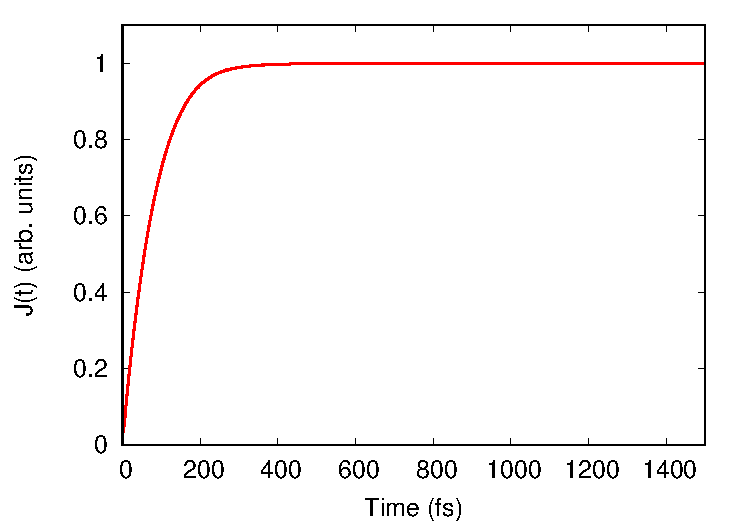
\includegraphics[width=0.8\linewidth]{pic/steady_current_appendix.pdf}
	\caption{\label{fig:steady}
		Electric current in graphene under a static electric field, $E_0=8.5$~MV/m. Figure is reproduced with permission from ref.~(\cite{PhysRevB.106.024313}). Copyright 2022, Phys. Rev. B.}
\end{figure}

As observed in Fig.\ref{fig:steady}, the application of the electric field induces an electric current at $t=0$, and it steadily approaches the steady-state value, denoted as $\mathbf J_S(E_0)$. This observation confirms that the electronic system, evolving under Eq.(\ref{eqn:masterequation}) with a static electric field, eventually reaches a nonequilibrium steady state after a sufficiently extended period of time propagation. This validation supports the reliability of the quasi-static approximation in capturing the nonequilibrium dynamics induced by a slowly varying electric field.
\begin{figure}[htbp]
	\centering
	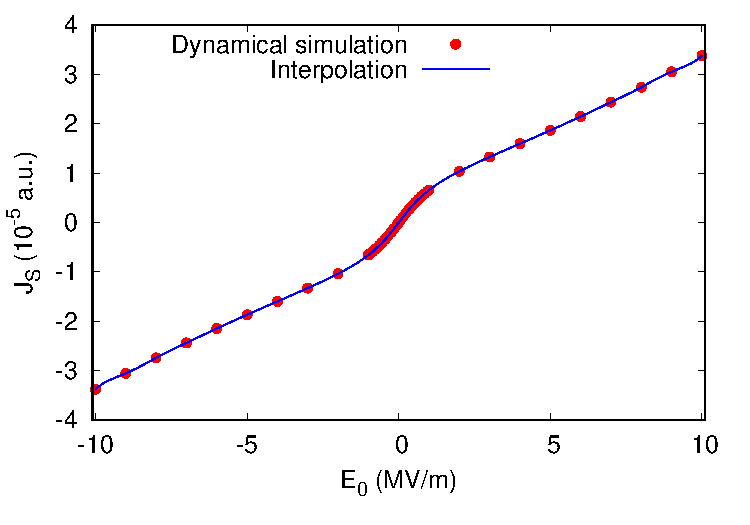
\includegraphics[width=0.8\linewidth]{pic/jsteady_interpolate.pdf}
	\caption{\label{fig:insert}
		Steady current $\mathbf J_S(E_0)$ as a function of field strength $E_0$. The results of the fully dynamical calculation are showns as the red points, while the interpolated result is shown as the blue-solid line. Figure is reproduced with permission from ref.~(\cite{PhysRevB.106.024313}). Copyright 2022, Phys. Rev. B.}
\end{figure}

In our practical simulations, we systematically vary the field strength $E_0$ and evaluate the resulting values of the steady current. Denoting the $k$th set of employed field strength and evaluated current as $E_k$ and $\mathbf J_k$ respectively, we represent the computed steady current $\mathbf J_k$ as red points in Figure~\ref{fig:insert} against the applied field strength $E_k$. To construct a continuous function $\mathbf J_S(E_0)$ from the discrete data points ${E_k, \mathbf J_k}$ in Figure~\ref{fig:insert}, we adopt a two-step interpolation procedure.

\begin{figure}[htbp]
	\centering
	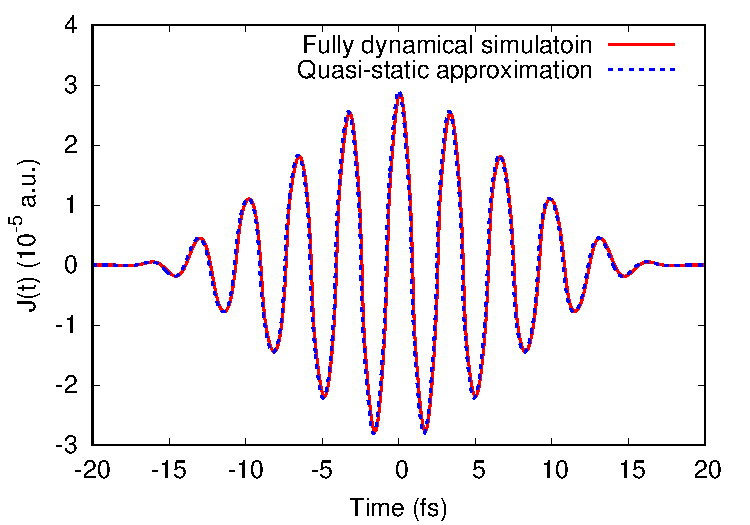
\includegraphics[width=0.8\linewidth]{pic/current_comparison_appendix.pdf}
	\caption{\label{fig:current} Comparison of the THz-induced current computed with the fully dynamical calculation and the quasi-static approximation. Figure is reproduced with permission from ref.~(\cite{PhysRevB.106.024313}). Copyright 2022, Phys. Rev. B.}
\end{figure}

In the first step of constructing the continuous function, we employ a polynomial regression with the following odd function:

\begin{align}
	\mathbf{J}_{\mathrm{polynomials }}(E_0)= \sum\limits{j=0}^{4} \mathbf e_x \alpha^{(2j+1)} E^{2j+1}_0,
	\label{eq:appendix-polynomial}
\end{align}

where $\alpha^{(j)}$ represents optimization parameters. These parameters are fine-tuned to ensure that the polynomial function $\mathbf{J}_{\mathrm{polynomials }}(E_0)$ effectively reproduces the discrete points ${E_k, \mathbf J_k}$ in Figure~\ref{fig:insert}.

Moving on to the second step, we aim to process the discrepancy between the discrete points in Figure~\ref{fig:insert} and the polynomial function $\mathbf{J}_{\mathrm{polynomials }}(E_0)$. To achieve this, we define the residual error of the polynomial regression as:

\begin{align}
	\Delta \mathbf{J}_k=\mathbf{J}_{k}-\mathbf{J}_{\mathrm{polynomials}}(E_k).
\end{align}

Subsequently, we apply spline interpolation to the data points ${E_k, \Delta \mathbf{J}k}$, denoting the interpolated function as $\Delta \mathbf{J}{\mathrm{spline}}(E_0)$. Finally, we approximate the continuous function, $\mathbf J_S(E_0)$, as:

\begin{align}
	\mathbf J_S(E_0)\approx \mathbf{J}_{\mathrm{polynomials }}(E_0)+\Delta \mathbf{J}_{\mathrm{spline}}(E_0).
	\label{eqn:approx}
\end{align}

\begin{figure}[htbp]
	\centering
	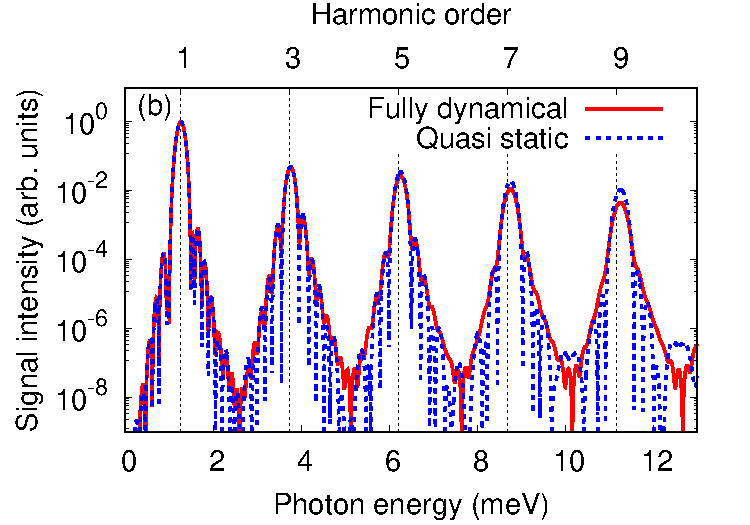
\includegraphics[width=0.8\linewidth]{pic/hhg_qstatic.pdf}
	\caption{\label{fig:hhg_qstatic}
		Comparison of the HHG spectra computed with the fully dynamical simulations in Sec.~\ref{subsec:dynamical_simulation} and the quasi-static approximation Sec.~\ref{subsec:quasi-static}. Here, the chemical potential is set to $\mu =170$~meV. Figure is reproduced with permission from ref.~(\cite{PhysRevB.106.024313}). Copyright 2022, Phys. Rev. B.}
\end{figure}

Utilizing the approximated function in Eq.(\ref{eqn:approx}), we evaluate the THz-induced electric
current with the quasi-static approximation, Eq.(\ref{eq:appendix-steady-current}).
The relationship between current and field as expressed in Eq.~(\ref{eq:steady-current}), we approximate the field-induced current $\mathbf J(t)$ by the steady-state current, where the instantaneous electric field is denoted as $\mathbf E(t)$, leading to the approximation $\mathbf J(t)\approx \mathbf J_S\left( \mathbf E(t) \right)$.
Figure~\ref{fig:current} showcases the computed current as a function of time with the quasi-static
approximation. To promote comparison, the result of the fully dynamical calculation is also
presented. Applying a Fourier transform to the obtained current in Figure~\ref{fig:current} yields
the \gls{HHG} spectra illustrated in Figure~\ref{fig:hhg_qstatic}.
%%%%%%%%%%%%%%%%%%%%%%%%%%%%%%%%%%%%%%%%%%%%%%%%%%%%%%%%%%%%%%%%%%%%%
\section{Nonlinear Charge Transport in Nonequilibrium Steady-state}
%%%%%%%%%%%%%%%%%%%%%%%%%%%%%%%%%%%%%%%%%%%%%%%%%%%%%%%%%%%%%%%%%%%%%%%%%%%%%%%%%%%%%%%%%%%%%%%%%%%%%%%%%%%%%%%%%%%%%%%%%%%%%%%%%%
To provide a broader context, we compare the nonequilibrium steady-state achieved within the quasi-static framework with insights collected from a recently developed thermodynamic model \cite{mics2015thermodynamic}. This comparative analysis aims to clarify the nonequilibrium mechanisms controlling nonlinear optical and transport phenomena within graphene in the THz regime. By contrasting the quasi-static nonequilibrium picture with the thermodynamic model, we endeavor to unravel the underlying dynamics driving the complex interplay between electron behavior and external THz fields in graphene systems.
We then study the nonlinear electric conductivity in a static regime in order to develop
microscopic insight into the THz-induced HHG. For this purpose, we first define the intraband
component of the steady-state current in Eq.~(\ref{eq:steady-current}).

Next, we proceed to evaluate the effective conductivities using both the total steady current
$\mathbf J_S(E_0)$ computed from Eq.~(\ref{eqn:totalcurrent})and the intraband component $\mathbf J^{\mathrm{intra}}_S(E_0)$ computed from Eq.~(\ref{eqn:intra-steady-current}). The effective total
and intraband conductivities are computed as follows:

\begin{align}
	\sigma(E_0)=\frac{\mathbf e_x\cdot \mathbf J_S(E_0)}{E_0} \quad, \\
	\quad \sigma^{\mathrm{intra}}(E_0)=\frac{\mathbf e_x\cdot \mathbf J^{\mathrm{intra}}_S(E_0)}{E_0}.
\end{align}

Figure~\ref{fig:conductivity} illustrates the computed effective conductivities, $\sigma(E_0)$ and $\sigma^{\mathrm{intra}}(E_0)$, as a function of the applied field strength $E_0$ for different chemical potentials $\mu$. In this figure, the conductivities $\sigma(E_0)$ obtained from the total steady current $\mathbf J_S(E_0)$ align well with those derived from the intraband current $ \mathbf J^{\mathrm{intra}}_S(E_0)$ across all investigated field strengths $E_0$ and chemical potentials $\mu$. This observation implies that the charge transport in graphene under static and THz fields is predominantly governed by the intraband current. The intraband current is described by the product of the band group velocity and the band population in the Brillouin zone.


\begin{figure}[htbp]
	\centering
	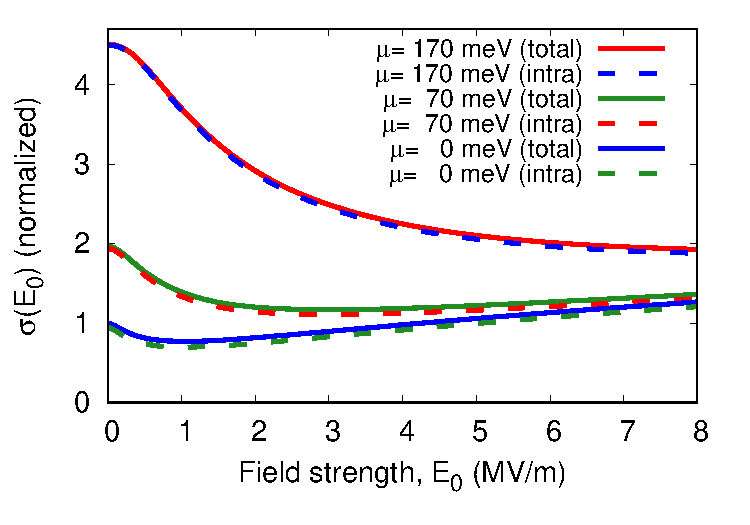
\includegraphics[width=0.8 \linewidth]{pic/sigma_vs_E0.pdf}
	\caption{\label{fig:conductivity}
		Nonlinear effective conductivities of graphene as a function of the static field strength $E_0$ evaluated with the total currents (solid lines) and intraband currents (dashed lines) for different values of the chemical potential, $\mu = 0$, $70$ and $170$~meV. Figure is reproduced with permission from ref.~(\cite{PhysRevB.106.024313}). Copyright 2022, Phys. Rev. B.}
\end{figure}

In Fig.~\ref{fig:conductivity}, the effective conductivities, $\sigma(E_0)$, show an initial
reduction across all investigated chemical potentials $\mu$ as the field strength increases from
zero. This reduction in conductivity combines with the field-induced transparency phenomenon observed
in graphene \cite{sato2021nonlinear}, as the conductivity $\sigma(E_0)$ is directly related to
photo absorption via Joule heating, given by:
\begin{align}
	E_{\mathrm{Joule}}=\mathbf E_0 \cdot \mathbf J_S(E_0)=\sigma(E_0)E^2_0
\end{align}
As the field strength continues to increase, graphene with relatively small chemical potentials (e.g., $\mu=0$ or $70$~meV) shows an increase in conductivity, while graphene with a relatively large chemical potential (e.g., $\mu=170$~meV) continues to show a reduction in conductivity. These trends are consistent with a previous theoretical study on nonlinear transport in graphene using the linear band approximation \cite{sato2021nonlinear}:
\begin{align}
	H_{\mathbf k}=v_F\left (\sigma_x k_x +\sigma_y k_y \right)
\end{align}
Given that the present work employs a more comprehensive electronic structure throughout the full Brillouin zone based on the tight-binding model, it serves as a validation of the low-energy Hamiltonian approximation for the graphene bandstructure used in the previous work. In the previous study \cite{sato2021nonlinear}, the decrease in effective conductivity was attributed to the dispersion of the population imbalance in the Brillouin zone, while the increase in conductivity was linked to additional carrier injection through the Zener tunneling mechanism. These interpretations naturally apply to the results obtained in the present study, further confirming the robustness and applicability of the previously proposed mechanisms.
\begin{figure}[htbp]
	\centering
	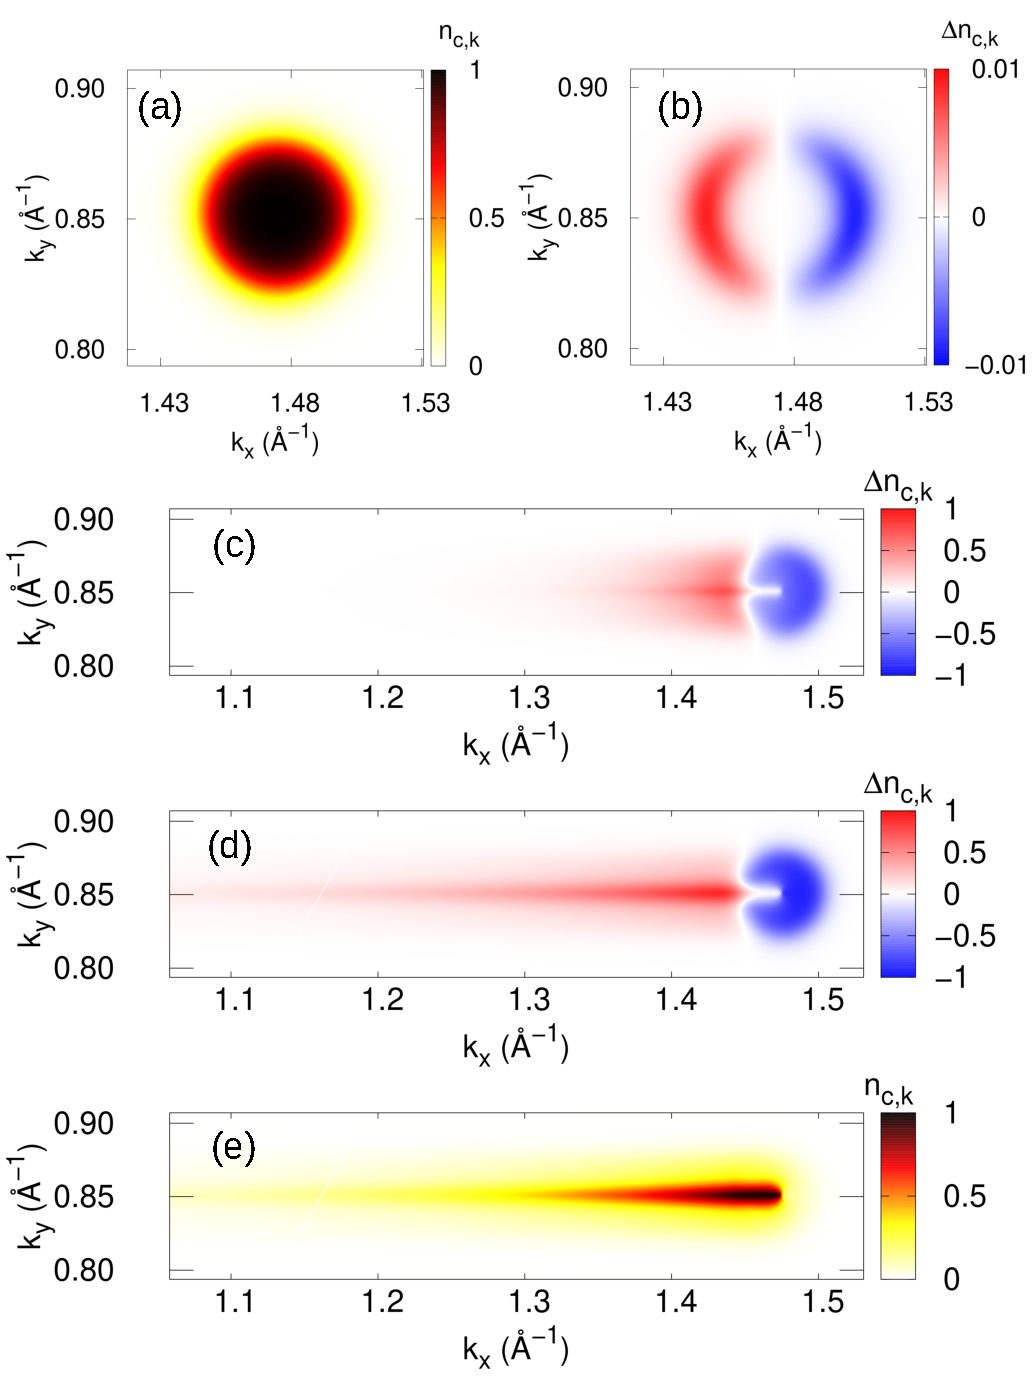
\includegraphics[width=1.0\linewidth]{pic/pop_fig.pdf}
	\caption{\label{fig:pop_f}
		(a) The equlibrium population distribution in the conduction band $f^{\mathrm{FD}}(\epsilon_{c,\mathbf k})$. (b-d) The field induced conduction population change for different field strengths, (b) $0.01$~MV/m, (c) $3$~MV/m, and (d) $10$~MV/m. (e) The population distribution in the conduction band in the nonequilibrium steady-state under a static field, $E_0=10$~MV/m. Panels are reproduced with permission from ref.~(\cite{PhysRevB.106.024313}). Copyright 2022, Phys. Rev. B.}
\end{figure}

Given the ability of the quasi-static approximation in accurately describing THz-induced electron
dynamics, the interpretation of THz-induced High-Order Harmonic Generation (HHG) finds its
foundation in the effective conductivities, as illustrated in Fig.~\ref{fig:conductivity}. The
conductivity $\sigma(E_0)$ remain saturated by the field strength $E_0$, the induced current
maintains linear proportionality to the field strength, thereby preventing the generation of
harmonics. Consequently, within the quasi-static framework, the emergence of harmonics arises from
the nonlinearity inherent in the current $\mathbf J_S(E_0)$ and the field-strength-dependent
conductivity $\sigma(E_0)$.

Examining Fig.\ref{fig:conductivity}, it becomes evident that the conductivity shows strengthened sensitivity to the field strength, particularly emphasized for larger chemical potentials. This emphasized dependence manifests as a pronounced reduction in conductivity with increasing field strength. This observation supports the explanation of the strengthened HHG in Fig.\ref{fig:hhg_mu} accompanying a shift in chemical potential—attributed to the significant reduction in conductivity coincident with the amplified field strength.

In former investigations \cite{hafez2018extremely,kovalev2021electrical}, the interpretation of THz-induced HHG in graphene was fixed in the reduction of conductivity, although within the framework of the thermodynamic model \cite{mics2015thermodynamic}. To unravel the influence of nonequilibrium dynamics in the steady state, we shall investigate into the interrelation between the two models—the nonequilibrium steady-state model and the thermodynamic model—in the forthcoming section, Sec.~\ref{sec:thermo}.

Moving to the intraband current presented in Eq.(\ref{eqn:intra-steady-current}), it is crucial to recognize its composition—encompassing the product of band velocity and population. Given the inherent invariance of band velocity under the presence of electric fields as an essential material property, the point of THz-induced current generation lies in the field-induced modulation of population. Furthermore, as explained earlier, the THz-induced current is predominantly governed by the intraband component. For an complex understanding of the THz-induced current at a microscopic level, we shall undertake an analysis of the population distribution within the Brillouin zone under the influence of the field. Figure\ref{fig:pop_f}~(a) describes the equilibrium population distribution in the conduction band, denoted as $f^{\mathrm{FD}}(\epsilon_{c,\mathbf k})$, Eq.~(\ref{eqn:fd-dist}), around a Dirac point (K point) in graphene, specifically at $K =\frac{2\pi}{\sqrt{3}a}\left(1, \frac{1}{\sqrt{3}}\right)$. Here, the chemical potential $\mu$ is established at $170$~meV. The equilibrium population shows a circular symmetry around the Dirac point, reflecting the partial filling of the Dirac cone by doped electrons.

We define the field-induced change in conduction population within a nonequilibrium steady
state as:
\begin{align}
	\Delta n_{c,\mathbf{k}}= \left [n_{c, \mathbf{k}'+e\mathbf{A}(t)/\hbar}(t)- f^{FD}(\epsilon_{c,\mathbf{k}'+e\mathbf A (t)/\hbar})\right ]_{\mathbf k'+e\mathbf A(t)/\hbar =\mathbf k}
\end{align}
Figures~\ref{fig:pop_f}~(b-d) showcase the field-induced conduction population $\Delta n{c,\mathbf{k}}$ for varying field strengths: (b)~$0.01$MV/m, (c)$3$MV/m, and (d)$10$~MV/m.

As illustrated in Fig.\ref{fig:pop_f}(b), the field-induced population modulation emerges along the
ring-shaped contour defined by the single-particle energy $\epsilon_{b\mathbf k}$ and the Fermi
energy $\epsilon_{\mathrm F}=\mu\big |_{T_e=0}$ as $\epsilon_{b\mathbf k}=\epsilon_{\mathrm F}$,
specifically where $\epsilon_{b \mathbf k}=\epsilon_{\mathrm F}$. The modulation occurs near to the Fermi energy due to the mild field excitation, and the ring structure derives from the circular symmetry inherent in the Dirac cone. In the weak field regime, the increasing and decreasing in conduction population $\Delta n_{c,\mathbf{k}}$ show symmetric distribution along the field direction ($x$-axis). On the contrary, in the strong-field regime, the distribution becomes non-symmetric, as evident in Figs.\ref{fig:pop_f}(c) and (d). Here, the red-colored region signifies an expanded range on the left side of the Dirac point, where population increase occurs, while the blue-colored region indicates a more confined area on the right side marked by population decrease. The population increase along the field direction may be construed as a consequence of the field-induced intraband acceleration within the Brillouin zone. Simultaneously, the localized population decrease around the Dirac point, as observed in Fig.\ref{fig:pop_f}(a), can be attributed to the field-induced displacement of initially localized electrons enveloping the Dirac point.

In the preceding study \cite{sato2021nonlinear}, the decrease in conductivity was clarifyd as the
saturation of population imbalance surrounding the Dirac point. To examine this interpretation,
we present the conduction population distribution:
\begin{align}
	n_{c,\mathbf k'+e\mathbf A(t)/\hbar}\big |_{\mathbf k'+e\mathbf A(t)/\hbar=\mathbf k}
\end{align}
in instead of the population change $\Delta n_{c,\mathbf{k}}$ in Fig.\ref{fig:pop_f}(e), with the field strength $E_0$ set to $10$MV/m. It is noteworthy that the summation of the density in Fig.\ref{fig:pop_f}(a) and the density change in Fig.\ref{fig:pop_f}(d) corresponds to the density in Fig.\ref{fig:pop_f}~(e).

Examining Fig.\ref{fig:pop_f}(e), a obviuos shift in the conduction population from the right to the left side of the Dirac cone is evident. This observation indicates that the population imbalance enveloping the Dirac cone is already near its maximum saturation point, where no further population can be transferred from the right side to the left side. Consequently, the population imbalance, a central determinant of the intraband current, reaches saturation in the strong-field regime, preventing any substantial increase. This saturation, in turn, leads to the saturation of the intraband current—predominant in the nonequilibrium steady state—finally ultimating in the observed reduction in conductivity within the strong-field regime.

Our investigation reveals a substantial decrease in the effective conductivity of graphene in the strong-field regime, attributed to the saturation of population imbalance within the Brillouin zone. This reduction combines with the observed THz-induced transparency in graphene, as reported experimentally \cite{Hwang2013, Paul_2013, doi:10.1063/1.4902999} and theoretically investigated in former studies \cite{sato2021nonlinear}. Furthermore, we establish that this diminished conductivity leads to nonlinear current behavior in the strong-field regime, ultimating in high-order harmonic generation in graphene. Thus, the origin of high-order harmonic generation can be understood through the lens of saturation of population displacement within the Brillouin zone in the context of nonequilibrium electron dynamics.
%%%%%%%%%%%%%%%%%%%%%%%%%%%%%%%%%%%%%%%%%%%%%%%%%%%%%%%%%%%%%%%%%%%%%%%%%%%%%%%%%%%%%%%%%%%%%%%%%%%%%%%%%%%%%%%%%%%%%%%%%%%%%%%%%%
\section{Comparison with Thermodynamic Model \label{sec:thermo}}
%%%%%%%%%%%%%%%%%%%%%%%%%%%%%%%%%%%%%%%%%%%%%%%%%%%%%%%%%%%%%%%%%%%%%%%%%%%%%%%%%%%%%%%%%%%%%%%%%%%%%%%%%%%%%%%%%%%%%%%%%%%%%%%%%%
Having clarifyd the microscopic intricacies of THz-induced \gls{HHG} in graphene within the framework of the none equilibrium steady-state, our focus now shifts to investigating the specific role played by the nonequilibrium nature of THz-induced electron dynamics. To accomplish this, we undertake a comparative analysis with the previously formulated thermodynamic model \cite{mics2015thermodynamic}. In contrast to the present nonequilibrium model, the thermodynamic model relies on the utilization of the thermal Fermi--Dirac distribution to delineate laser-excited electronic systems. This model operates under the assumption that electrons swiftly undergo thermalization, allowing them to be effectively treated as an equilibrium state characterized by a notably high electron temperature $T_e$.

\begin{figure}[htbp]
	\centering
	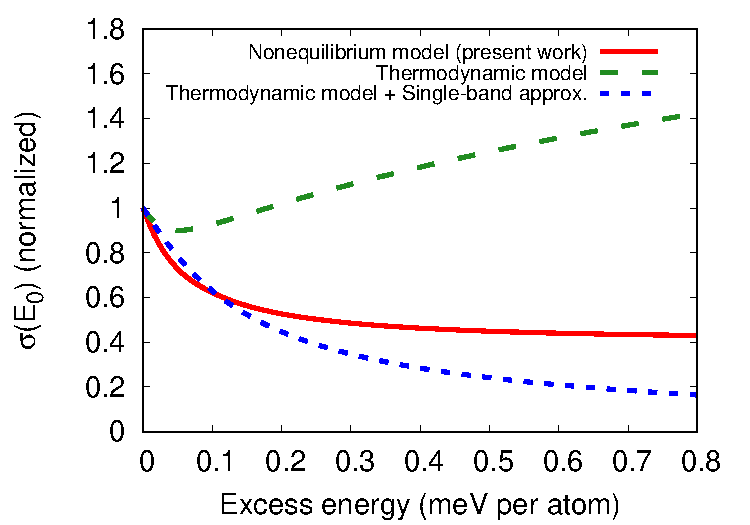
\includegraphics[width=0.8\linewidth]{pic/sigma_thermo.pdf}
	\caption{\label{fig:compare} Computed effective conductivities are shown as a function of the excess energy. The results for the nonequilibrium steady-state (red-solid), the thermodynamic model (green-dashed), and the thermodynamic model plus the single-band approximation (blue-dotted) are shown. Figure is reproduced with permission from ref.~(\cite{PhysRevB.106.024313}). Copyright 2022, Phys. Rev. B.}
\end{figure}

Within the thermodynamic model, equilibrium states find characterization through the electron
temperature $T_e$, while in the developed nonequilibrium model, nonequilibrium steady-states are
essentialally defined by the applied field strength $E_0$, devoid of any reliance on temperature
considerations. To ensure a equitable comparison between the two models, it becomes imperative to
establish a connection between the electron temperature $T_e$ and the field strength $E_0$. This connection is promoted by the introduction of the field-induced excess energy for each model.

The total energy of the electronic system is formulated as:
\begin{eqnarray}
	E_{\mathrm{tot}}(t)=\frac{2}{(2\pi)^2} \int d\mathbf k \mathrm{Tr}\left[H_{\mathbf k+ e\mathbf A(t)/\hbar} \rho_{\mathbf k}(t)\right].
	\label{eqn:totalenergy}
\end{eqnarray}

Subsequently, the field-induced excess energy of the nonequilibrium steady-state is defined as
\begin{eqnarray}
	\Delta E^\mathrm{NEQ}_{\mathrm{excess}}(E_0)=\lim_{t\rightarrow \infty} \left [E_{\mathrm{tot}}(t)
	-E_{\mathrm{tot}}(-t) \right ],
	\label{eq:excess-energy-neq}
\end{eqnarray}

Here, $\lim_{t\rightarrow \infty} E_{\mathrm{tot}}(t)$ corresponds to the total energy in the nonequilibrium steady-state under the presence of the field $E_0$, while $\lim_{t\rightarrow \infty} E_{\mathrm{tot}}(-t)$ corresponds to that of the equilibrium state without the field. Thus, the field-induced excess energy of the nonequilibrium model captures the energy difference between the nonequilibrium steady-state under an external field $E_0$ and the field-free equilibrium state.

In contrast, the field-induced excess energy of the thermodynamic model is defined as the energy difference between finite temperature states at $T_e$ and $300$K, the initial temperature of the present nonequilibrium model:
\begin{align}
	\Delta E^\mathrm{TM}_{\mathrm{excess}} & =\sum_{b=v,c}\frac{2}{(2\pi)^2}\int d\mathbf k
	\epsilon_{b\mathbf k} \nonumber                                                         \\
	                                       & \times \left [
	f^{\mathrm{FD}}\left (\epsilon_{b\mathbf k},T_e,\mu \right )
	-f^{\mathrm{FD}}\left (\epsilon_{b\mathbf k},T_e=300~\mathrm{K},\mu \right )
	\right ].
	\label{eq:excess-energy-tm}
\end{align}

Therefore, $\Delta E^\mathrm{TM}_{\mathrm{excess}}$ is expressed as a function of the electron
temperature $T_e$.

By employing Eq.(\ref{eq:excess-energy-neq}) and Eq.(\ref{eq:excess-energy-tm}), we establish a link between the applied field strength $E_0$ characterizing the nonequilibrium steady-state and the electron temperature $T_e$ inherent to the thermodynamic model through the concept of excess energy. This connection enables a comparative analysis of the effective conductivity $\sigma(E_0)$ in the nonequilibrium steady-state and the linear conductivity of the thermodynamic model.

Figure~\ref{fig:compare} presents the conductivities of the nonequilibrium steady-state (illustrated
by the red-solid line) and the thermodynamic model (represented by the green-dashed line). The
computations for the nonequilibrium steady-state consider a chemical potential $\mu$ set to
$170$~meV and an electron temperature $T_e$ in the relaxation operator set to $300$~K. In contrast,
the linear conductivity of the thermodynamic model is evaluated under the influence of a weak
field, ensuring the induced current combines with a linear response. The results for the
thermodynamic model involve varying the electron temperature $T_e$ while maintaining the total
population constant, as expressed by:
\begin{align}
	N_{\mathrm{tot}}=\frac{2}{(2\pi)^2}\sum_{b=v,c} \int d\mathbf k f^{FD}(\epsilon_{b\mathbf k},T_e,\mu),
	\label{eq:tot-pop}
\end{align}
to the value at $T_e=300$~K and $\mu=170$~meV. Consequently, the chemical potential goes through adjustments with changes in the electron temperature.

Figure~\ref{fig:compare} illustrates that the conductivity of the thermodynamic model (represented by the green-dashed line) initially experiences a decrease with an increase in the excess energy, followed by a notable upturn once the excess energy reaches a fairly large value. In contrast, the conductivity of the nonequilibrium steady-state (represented by the red-solid line) consistently decreases with the increase of the excess energy across the entire explored range. It's important to note that the conductivity of the nonequilibrium steady-state in Fig.\ref{fig:compare} combines with that in Fig.\ref{fig:conductivity} when considering the converted $x$-axis. The fundamental contrast between the conductivities of the nonequilibrium steady-state and the thermodynamic model arises from the interband excitation influenced by temperature. In the thermodynamic model, thermal excitation drives electrons from the valence band to the conduction band, enhancing effective carrier population and subsequently enhancing conductivity with elevated electron temperatures. In contrast, the nonequilibrium steady-state experiences a significant suppression of field-induced interband excitation due to Pauli blocking, moderating the artificial rise in effective carrier population and the resultant increase in conductivity.

In previous study \cite{mics2015thermodynamic}, the authors investigated into the microscopic intricacies of THz-induced high-order harmonic generation and field-induced transparency in graphene using the thermodynamic model. Notably, the investigation adopted a single-band approximation in which only the conduction band was considered, while the valence band remained frozen. Surprisingly, this single-band approximation showed better agreement with experimental results than the two-band approximation, where both valence and conduction bands were considered \cite{kovalev2021electrical}. Despite the instinctive expectation that the two-band approximation would offer greater accuracy, the results indicated that the single-band approximation provided a more accurate picture within the thermodynamic model.

To clarify the role of the single-band approximation in the thermodynamic model, we extended our comparison between the thermodynamic model and the nonequilibrium steady-state by considering the single-band approximation into our analysis. In this adaptation, we phenomenologically constrained the population in the valence band, while maintaining the use of the Fermi--Dirac distribution for the conduction band. This modification involved transforming the Fermi--Dirac distribution as follows:
\begin{align}
	\tilde f^{\mathrm{MFD}}(\epsilon, T_e, \mu)=f^{\mathrm{FD}}(\epsilon, T_e, \mu)\Theta(\epsilon)+\Theta(-\epsilon),
	\label{eq:mod-fd-dist}
\end{align}
where $\Theta(\epsilon)$ represents the Heaviside step function. By replacing the original Fermi--Dirac distribution (Eq.(\ref{eq:fd-dist})) with the modified version (Eq.(\ref{eq:mod-fd-dist})), we conducted a comparative analysis of conductivity with the thermodynamic model. The results of the thermodynamic model considering the single-band approximation are illustrated by the blue-dotted line in Fig.~\ref{fig:compare}. Remarkably, this modified thermodynamic model effectively reproduces the conductivity trend observed in the nonequilibrium steady-state, showcasing a consistent monotonic decrease with an increase in excess energy.

This interesting outcome suggests that the freezing of the valence band in the single-band approximation decreases the artificial interband excitation in the thermodynamic model, leading to a more accurate performance of conductivity. In contrast, the nonequilibrium steady-state, based on a fully dynamical model, naturally captures the suppression of interband excitation, providing an accurate representation of electron dynamics in graphene under THz fields without resorting to the freezing of the valence band.

Consequently, our findings indicate that the thermodynamic model shows an enhancement of electric conductivity when subjected to intense THz fields, originating from interband transitions between the valence and conduction bands. To compare with former thermodynamic model\cite{kovalev2021electrical}, we introduced a single-band approximation, freezing the valence band to forbid interband excitation. Correspondingly, the computed conductivity in the thermodynamic framework, employing this single-band approximation, accurately reflects the anticipated decreasing trend under static field radiation. This trend combines with experimental observations of the field-induced transparency of graphene \cite{Hwang2013, Paul_2013, doi:10.1063/1.4902999}. In contrast, the nonequilibrium model developed in this study effectively captures the decreasing trend in conductivity under static field irradiation without the need for artificially freezing the valence band. This emphasized the essential role of the nonequilibrium nature of electron dynamics in describing conductivity reduction under electric field irradiation and preventing interband excitation, as evidenced in the comparison with the thermodynamic model.

%\chapter{ENHANCEMENT OF MIR-INDUCED HHG BY COHERENT COUPLING WITH THZ FIELD}
\section{Orientational dependence of HHG}
\section{Comparison of the nonequilibrium steady state and the thermodynamic model}
\section{Contribution of the nonequilibrium population}
\appendix
\chapter{ADIABATIC BASIS REPRESENTATION \label{ch:A_ADIABATIC}}
\label{ch:Adiabatic}
The adiabatic approximation is used almost all the time in solving time-propagation, which will be
explained in more detail here.
To analytically investigate nonlinear photocarrier injection in solids, we first introduce the equation of motion in the adiabatic basis representation. In this representation, we can naturally separate the interband transitions, the dynamical phase factor, and the geometric phase factor. To introduce the representation, we consider the following one-body Schr\"odinger equation for a $\mathbf k$-point,
\begin{equation}
	i \frac{d}{dt} | \psi_{\mathbf k}(t) \rangle = H \left [\mathbf k + \mathbf A(t) \right ] | \psi_{\mathbf k}(t) \rangle,
	\label{eqn:tdse00}
\end{equation}
where $\mathbf A(t)$ is an external vector potential, which is related to the external electric field as $\mathbf E(t)=-d\mathbf A(t)/dt$. In this note, we assume that the vector potential is zero for the negative time; $\mathbf A(t\leq 0)=0$.

To introduce the adiabatic basis representation, we introduce the instantaneous eigenstates of the Hamiltonian as
\begin{align}
	H\left [\mathbf k + \mathbf A(t) \right ] |u_{b,\mathbf k+\mathbf A(t)}\rangle = \epsilon_{b,\mathbf k + \mathbf A(t)}|u_{b,\mathbf k+\mathbf A(t)}\rangle,
	\label{eq:static-se}
\end{align}
where $b$ is the band index. Hereafter, we assume the two-band system, which has the valence band ($b=v$) and the conduction band ($b=c$). However, we can straightforwardly extend it to general systems.

On the basis of the instantaneous eigenstates defined by Eq.~(\ref{eq:static-se}), we consider the following expansion of the wavefunction
\begin{align}
	|\psi_{\mathbf k}(t)\rangle = c_{v,\mathbf k}(t) e^{-i\int^t_0dt' \epsilon_{v,\mathbf k+ \mathbf A(t')}} e^{i\phi^g_{v,\mathbf k}(t)} |u_{v,\mathbf k+\mathbf A(t)}\rangle
	+c_{c,\mathbf k}(t) e^{-i\int^t_0dt' \epsilon_{c,\mathbf k+ \mathbf A(t')}} e^{i\phi^g_{c,\mathbf k}(t)} |u_{c,\mathbf k+\mathbf A(t)}\rangle,
	\label{eq:ansatz}
\end{align}
where $c_{b,\mathbf k}(t)$ are the expansion coefficients. In the expansion, we explicitly include the dynamical phase factor, $e^{-i\int^t_0dt' \epsilon_{v,\mathbf k+ \mathbf A(t')}}$, and the additional phase factor, $e^{i\phi^g_{b,\mathbf k}(t)}$. The latter one will be defined later as the geometric phase factor.

Inserting Eq.~(\ref{eq:ansatz}) into Eq.~(\ref{eq:tdse00}), one obtains
\begin{align}
	\left [i\frac{d}{dt}-H\left [\mathbf k + \mathbf A(t) \right ] \right ]|\psi_{\mathbf k}(t) \rangle & =
	i \dot c_{v,\mathbf k}(t) e^{-i\int^t_0dt' \epsilon_{v,\mathbf k+ \mathbf A(t')}} e^{i\phi^g_{v,\mathbf k}(t)} |u_{v,\mathbf k+\mathbf A(t)}\rangle \nonumber                                                                                                                                                          \\
	                                                                                                    & + i\dot c_{c,\mathbf k}(t) e^{-i\int^t_0dt' \epsilon_{c,\mathbf k+ \mathbf A(t')}} e^{i\phi^g_{c,\mathbf k}(t)} |u_{c,\mathbf k+\mathbf A(t)}\rangle \nonumber                                                   \\
	                                                                                                    & - \dot \phi^g_{v,\mathbf k}(t) c_{v,\mathbf k}(t) e^{-i\int^t_0dt' \epsilon_{v,\mathbf k+ \mathbf A(t')}} e^{i\phi^g_{v,\mathbf k}(t)} |u_{v,\mathbf k+\mathbf A(t)}\rangle \nonumber                            \\
	                                                                                                    & - \dot \phi^g_{c,\mathbf k}(t) c_{c,\mathbf k}(t) e^{-i\int^t_0dt' \epsilon_{c,\mathbf k+ \mathbf A(t')}} e^{i\phi^g_{c,\mathbf k}(t)} |u_{c,\mathbf k+\mathbf A(t)}\rangle \nonumber                            \\
	                                                                                                    & - i c_{v,\mathbf k}(t) e^{-i\int^t_0dt' \epsilon_{v,\mathbf k+ \mathbf A(t')}} e^{i\phi^g_{v,\mathbf k}(t)} \mathbf E(t)\cdot \frac{\partial |u_{v,\mathbf k+\mathbf A(t)}\rangle}{\partial \mathbf k} \nonumber \\
	                                                                                                    & - i c_{c,\mathbf k}(t) e^{-i\int^t_0dt' \epsilon_{c,\mathbf k+ \mathbf A(t')}} e^{i\phi^g_{c,\mathbf k}(t)} \mathbf E(t)\cdot \frac{\partial |u_{c,\mathbf k+\mathbf A(t)}\rangle}{\partial \mathbf k} = 0.
	\label{eq:tdse01}
\end{align}

By multiplying $e^{+i\int^t_0dt' \epsilon_{v,\mathbf k+ \mathbf A(t')}} e^{-i\phi^g_{v,\mathbf k}(t)} \langle u_{v,\mathbf k+\mathbf A(t)}|$ to Eq.~(\ref{eq:tdse01}), one obtains
\begin{align}
	 & i \dot c_{v,\mathbf k}(t) - \dot \phi^g_{v,\mathbf k}(t) c_{v,\mathbf k}(t) - i c_{v,\mathbf k}(t) \mathbf E(t)\cdot \left \langle u_{v,\mathbf k+\mathbf A(t)}\Big |\frac{\partial u_{v,\mathbf k+\mathbf A(t)}}{\partial \mathbf k} \right \rangle \nonumber \\
	 & - i c_{c,\mathbf k}(t) e^{-i\int^t_0dt' \epsilon_{c,\mathbf k+ \mathbf A(t')}-\epsilon_{v,\mathbf k+ \mathbf A(t')}} e^{i\left (\phi^g_{c,\mathbf k}(t)-\phi^g_{v,\mathbf k}(t)\right )}
	\mathbf E(t)\cdot \left \langle u_{v,\mathbf k+\mathbf A(t)}\Big |\frac{\partial u_{c,\mathbf k+\mathbf
	A(t)}}{\partial \mathbf k} \right \rangle                                                                                                                                                                                                                         \\& = 0.
	\label{eq:eom-valence}
\end{align}

Likewise, by multiplying $e^{+i\int^t_0dt' \epsilon_{c,\mathbf k+ \mathbf A(t')}} e^{-i\phi^g_{c,\mathbf k}(t)} \langle u_{c,\mathbf k+\mathbf A(t)}|$ to Eq.~(\ref{eq:tdse01}), one obtains
\begin{align}
	 & i \dot c_{c,\mathbf k}(t) - \dot \phi^g_{c,\mathbf k}(t) c_{c,\mathbf k}(t) - i c_{c,\mathbf k}(t) \mathbf E(t)\cdot \left \langle u_{c,\mathbf k+\mathbf A(t)}\Big |\frac{\partial u_{c,\mathbf k+\mathbf A(t)}}{\partial \mathbf k} \right \rangle \nonumber \\
	 & - i c_{v,\mathbf k}(t) e^{-i\int^t_0dt' \epsilon_{v,\mathbf k+ \mathbf A(t')}-\epsilon_{c,\mathbf k+ \mathbf A(t')}} e^{i\left (\phi^g_{v,\mathbf k}(t)-\phi^g_{c,\mathbf k}(t)\right )}
	\mathbf E(t)\cdot \left \langle u_{c,\mathbf k+\mathbf A(t)}\Big |\frac{\partial u_{v,\mathbf k+\mathbf A(t)}}{\partial \mathbf k} \right \rangle = 0.
	\label{eq:eom-conduction}
\end{align}

Combining Eq.~(\ref{eq:eom-valence}) and Eq.~(\ref{eq:eom-conduction}), one can obtain the following matrix form,
\begin{align}
	 & i\frac{d}{dt} \mathbf c_{\mathbf k}(t) =
	\left(
	\begin{array}{cc}
			\dot \phi^g_{v,\mathbf k}(t) &
			0                              \\
			0                            &
			\dot \phi^g_{c,\mathbf k}(t)
		\end{array}
	\right) \mathbf c_{\mathbf k}(t)
	+i\mathbf E(t)\cdot \left(
	\begin{array}{cc}
			M_{11} & M_{12} \\
			M_{21} & M_{22}
		\end{array}
	\right) \mathbf c_{\mathbf k}(t),
\end{align}

\begin{align}
	 & M_{11} = \left \langle u_{v,\mathbf k+\mathbf A(t)}\Big |\frac{\partial u_{v,\mathbf k+\mathbf
	A(t)}}{\partial \mathbf k} \right \rangle                                                                                                   \\
	 & M_{12} = e^{-i\int^t_0dt' \Delta \epsilon_{cv,\mathbf k+ \mathbf A(t')}+i \Delta \phi^g_{cv,\mathbf k}(t)}
	\left \langle u_{v,\mathbf k+\mathbf A(t)}\Big |\frac{\partial u_{c,\mathbf k+\mathbf A(t)}}{\partial
	\mathbf k} \right \rangle                                                                                                                   \\
	 & M_{21} = e^{-i\int^t_0dt' \Delta \epsilon_{vc,\mathbf k+ \mathbf A(t')}+i \Delta \phi^g_{vc,\mathbf k}(t)}
	\left \langle u_{c,\mathbf k+\mathbf A(t)}\Big |\frac{\partial u_{v,\mathbf k+\mathbf A(t)}}{\partial
	\mathbf k} \right \rangle                                                                                                                   \\
	 & M_{22} = \left \langle u_{v,\mathbf k+\mathbf A(t)}\Big |\frac{\partial u_{v,\mathbf k+\mathbf A(t)}}{\partial \mathbf k} \right \rangle
\end{align}

where $\Delta\epsilon_{bb',\mathbf k+ \mathbf A(t)}$ is defined by the difference of the single particle energies as $\epsilon_{b,\mathbf k+ \mathbf A(t)}-\epsilon_{b',\mathbf k+ \mathbf A(t)}$, and $\Delta \phi^g_{bb',\mathbf k}(t)$ is defined by the difference of the geometric phases as $\phi^g_{b,\mathbf k}(t)-\phi^g_{b',\mathbf k}(t)$. Here, the coefficient vector was introduced as
\begin{align}
	\mathbf c_{\mathbf k}(t) = \left(
	\begin{array}{cc}
			c_{v,\mathbf k}(t) \\
			c_{c,\mathbf k}(t)
		\end{array}
	\right).
\end{align}

Here, we define the geometric phases as
\begin{align}
	\phi^g_{b,\mathbf k}(t) & = -i\int^t_0 dt' \mathbf E(t')\cdot
	\left \langle u_{b,\mathbf k+\mathbf A(t')}\Big |\frac{\partial u_{b,\mathbf k+\mathbf A(t')}}{\partial
	\mathbf k} \right \rangle                                                                                                                                                                                     \\
	                        & =i\int^t_0 dt' \frac{dA(t')}{dt'}\cdot
	\left \langle u_{b,\mathbf k+\mathbf A(t')}\Big |\frac{\partial u_{b,\mathbf k+\mathbf A(t')}}{\partial \mathbf k} \right \rangle \nonumber                                                                   \\
	                        & = i \oint^{\mathbf A(t)}_{\mathbf A(0)} d\mathbf A \cdot \left \langle u_{b,\mathbf k+\mathbf A}\Big |\frac{\partial u_{b,\mathbf k+\mathbf A}}{\partial \mathbf k} \right \rangle.
	\label{eq;geometric-phase}
\end{align}
As seen from the last expression in Eq.~(\ref{eq;geometric-phase}), the phase $\phi^g_{b,\mathbf k}$ depends only on the geometry of the path of the integral.

With the expression of the geometric phases in Eq.~(\ref{eq;geometric-phase}), one can rewrite the equation of motion for the coefficient vector as
\begin{align}
	 & i\frac{d}{dt} \mathbf c_{\mathbf k}(t) = \mathcal{H}(t) \mathbf c_{\mathbf k}(t)
	.
	\label{eq:tdse-ad-basis_A}
\end{align}
\begin{align}
	 & \mathcal{H}(t)=
	i\mathbf E(t)\cdot \left(
	\begin{array}{cc}
			0      & M_{12} \\
			M_{21} & 0
		\end{array}
	\right)
\end{align}

This is the time-dependent Schr\"odinger equation on the adiabatic basis, and it is closely related to the Houston basis expansion \cite{PhysRev.57.184,PhysRevB.33.5494}.


%\include{chapter/A_math}
\backmatter
\begingroup
    \onehalfspacing
    \printbibliography[heading=bibintoc]
\endgroup
\end{document}
